\documentclass[a4paper]{fhnwreport} 
\usepackage[german]{babel}
\usepackage[babel, german=quotes]{csquotes}
\usepackage{hyperref}
\usepackage{verbatim}
\usepackage{amsmath}		
\usepackage{amsthm}		
\usepackage{graphicx} 	
\usepackage{fancyhdr}
\usepackage[latin1]{inputenc}
\usepackage[T1]{fontenc}
\usepackage{pdfpages}
\usepackage{tikz}
\usetikzlibrary{arrows}
\usepackage{lmodern}
\usepackage{listings}
\usepackage{subfigure}	
\usepackage{booktabs}		
\usepackage{todonotes}	
\usepackage{cite}			
%\usepackage{tabularx}
%\uspackage{listings}		% Paket f�r die Dokumentierung von Software-Code
\lstset{language=Matlab}



% Farben f�r Matlab-Listings
\definecolor{hellgelb}{rgb}{1,1,0.85}     % Hintergrundfarbe
\definecolor{colKeys}{RGB}{0,0,255}       % blau
\definecolor{colIdentifier}{RGB}{0,0,0}	  % schwarz
\definecolor{colComments}{RGB}{34,139,34} % gruen
\definecolor{colString}{RGB}{160,32,240}  % violett

\lstset{%
    language=Matlab,%
    %backgroundcolor={\color{hellgelb}},%
		backgroundcolor={},%
    basicstyle={\footnotesize\ttfamily},%
    breakautoindent=true,%
    breakindent=10pt,%
    breaklines=true,%
    captionpos=t,%
    columns=fixed,%
    %commentstyle={\itshape\color{colComments}},%
		commentstyle={\color{colComments}},
    extendedchars=true,%
    float=hbp,%
    frame=single,%
    framerule=1pt,%
    identifierstyle={\color{colIdentifier}},%
    keywordstyle={\color{colKeys}},%
    numbers=left,%
    numbersep=1em,%
    numberstyle={\tiny\ttfamily},%
    showspaces=false,%
    showstringspaces=false,%
    stringstyle={\color{colString}},%
    tabsize=4,%
    xleftmargin=1em,%
    xrightmargin=1em%
} 

\bibliographystyle{IEEEtran}	
%\graphicspath{{./graphics/}{./Anhang/}}	
\geometry{twoside=false}	
\overfullrule=1em	

\title{Fachbericht Easy-PID}
\date{Windisch, \today}

\graphicspath{{./Bilder/}}

\begin{document}
\maketitle

\vspace*{2cm}
\begin{figure}[h]
	\centering
		
\includegraphics[width=0.80\textwidth]{easypid-logo.png}
	\label{fig:easypid-logo}
\end{figure}
\vfill
\textsc{
\begin{tabbing}
Auftraggeber: \hspace{4em} \=   Peter Niklaus \\[2ex]
Betreuer:  \>  Peter Niklaus (Elektrotechnik) \\ \> Richard Gut (Objektorientierte Programmierung) \\ \> Pascal Buchschacher (Projektmanagement) \\ \> Anita Gertiser (Kommunikation) \\[2ex]
Gruppe:  \>  FS15 pro2E Team 3 \\[2ex]
Teammitglieder:  \> Yanick Frei (Projektleiter) \\ \> Simon Wyss (Experte Elektrotechnik) \\ \> Josua Stierli (Experte Programmierung) \\ \> Alexander Murray (Stv. Projektleiter) \\ \> Simon Sturm \\[2ex]
Studiengang: \> Elektro- und Informationstechnik
\end{tabbing}}
\vfill
\hbox{}
\clearpage


\includepdf[pages=-]{Abstract.pdf}

\includepdf[pages=-]{P2_FS_2015_Aufgabe_vom_Auftraggeber.pdf} 
\setcounter{page}{1}
\tableofcontents	
\clearpage

\section{Einleitung}
Das Berechnen von Reglern ist oftmals eine schwierige Angelegenheit, die sowohl Erfahrung als auch Zeit ben�tigt. Zur richtigen Dimensionierung helfen entweder Faustformeln oder auch grafische Methoden, welche jedoch von Hand ausgef�hrt werden m�ssen. Folglich ist die Berechnung entweder ungenau oder sehr aufw�ndig. Da es fragw�rdig ist, ob solch manuelle Methoden in einer Zeit von Matlab und weiteren Berechnungstools noch zeitgem�ss sind, wurde im Projekt 2 eine Software erstellt, welche Regler automatisch anhand der "`Phasengangmethode zur Reglerdimensionierung"' von Jakob Zellweger dimensionieren kann.

Das Hauptziel des Projektes war es, ein funktionierendes Programm zu erstellen, welches die Reglerberechnung automatisch nach der Phasengangmethode von Zellweger sowie weiteren Faustformeln dimensioniert. Zur korrekten Funktion werden sowohl richtig implementierte Berechnungen ben�tigt als auch die richtige Darstellung der Ergebnisse, beispielsweise mittels sinnvoll skalierten Graphen. Ausserdem wurden einige optionale Ziele definiert. Die wichtigsten davon sind die Simulation der geschlossenen Regelstrecke, eine Miniversion des Programms sowie eine M�glichkeit zum Nachjustieren der Eingabeparameter.

Easy-PID ist ein Programm, mit welchem Regler anhand der Parameter der Schrittantwort automatisch dimensioniert werden k�nnen. Easy-PID besitzt ausserdem ein intuitiv zu bediendendes User-Interface, welches neben den Ein- und Ausgabeparemetern auch das dynamische Verhalten des Regelkreises, welche mit verschiedenen Methoden berechnet wurde, grafisch darstellt. Durch die verschiedenen Dimensionerungsmethoden und der M�glichkeit, Parameter in Echtzeit zu manipulieren, kann ein optimaler Regler gefunden werden.

Dieser Bericht beschreibt die Probleml�sung aufgeteilt auf die drei Teilbereiche Elektrotechnik, Porgrammierung und Validierung. Der Elektrotechnische Teil behandelt die hergeleiteten Formeln f�r die Reglerdimensionierung und die Programmierung dieser Formeln in Matlab, w�hrend der zweite Teil den Aufbau der Benutzeroberfl�che und die Umsetzung der Matlab-Programmierung in Java behandelt. Die Validierung beschreibt den Aufbau und den Vorgang der Tests sowie deren Ergebnisse.

%\include{Disposition}


%\documentclass{fhnwreport} %
%\usepackage[ngerman]{babel}
%\usepackage[T1]{fontenc}
%\usepackage[latin1]{inputenc}
%\usepackage{tikz}
%\usepackage{amsmath}
%\usetikzlibrary{arrows}
%\usepackage{lmodern}   %Type1-Schriftart f�r nicht-englische Texte 
%
%\usepackage{listings}
%\lstset{language=Matlab}
%
%\usepackage{color}

%% Farben f�r Matlab-Listings
%\definecolor{hellgelb}{rgb}{1,1,0.85}     % Hintergrundfarbe
%\definecolor{colKeys}{RGB}{0,0,255}       % blau
%\definecolor{colIdentifier}{RGB}{0,0,0}	  % schwarz
%\definecolor{colComments}{RGB}{34,139,34} % gruen
%\definecolor{colString}{RGB}{160,32,240}  % violett
%
%\lstset{%
    %language=Matlab,%
    %%backgroundcolor={\color{hellgelb}},%
		%backgroundcolor={},%
    %basicstyle={\footnotesize\ttfamily},%
    %breakautoindent=true,%
    %breakindent=10pt,%
    %breaklines=true,%
    %captionpos=t,%
    %columns=fixed,%
    %%commentstyle={\itshape\color{colComments}},%
		%commentstyle={\color{colComments}},
    %extendedchars=true,%
    %float=hbp,%
    %frame=single,%
    %framerule=1pt,%
    %identifierstyle={\color{colIdentifier}},%
    %keywordstyle={\color{colKeys}},%
    %numbers=left,%
    %numbersep=1em,%
    %numberstyle={\tiny\ttfamily},%
    %showspaces=false,%
    %showstringspaces=false,%
    %stringstyle={\color{colString}},%
    %tabsize=4,%
    %xleftmargin=1em,%
    %xrightmargin=1em%
%} 
%\graphicspath{{./PrettyPictures}} 
%
%\begin{document}
\section{Elektrotechnische Probleml�sung}\label{ETProblemsolving}
In diesem Kapitel wird das Vorgehen zur Elektrotechnischen Probleml�sung genauer erl�utert. Dabei wird n�her auf die Grundlagen der Regelungstechnik, die Zellweger-Methode, einige Faustformeln und das Berechnen des geschlossenen Regelkreises eingegangen.

\subsection{Regelungstechnische Grundlagen}\label{RegelGrundlagen}
Ein Regelkreis besteht aus einer Strecke und einem Regler.

\begin{figure}[h]%Bild eines gesamten Regelkreises(Wikipedia):http://de.wikipedia.org/wiki/Regelkreis#/media/File:Einfacher_Regelkreis_n.svg
\centering
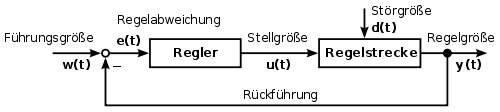
\includegraphics[width=0.8\textwidth]{./Einfacher_Regelkreis_Wikipedia.png}
\caption{Regler und Regelstrecke\cite{RegelKreisWikipedia}}
\label{fig:Reglerstrecke}
\end{figure}

Die Aufgabe des Reglekreises ist, es die Regelgr�sse konstant auf dem Wert der sogenannten F�hrungsgr�sse zu halten. Bei einer Heizung w�ren dies beispielsweise die momentane Temperatur, die auf die gew�nschte Temperatur zu regeln ist. Die Strecke w�re dabei der zu heizende Raum und der Regler die Heizung selbst.

Um den Regelkreis beschreiben zu k�nnen braucht man zun�chst die Schrittantwort der Strecke. Aus dieser kann man nun mithilfe der Wendetangentenmethode die Parameter $Ks$ (Verst�rkungsfaktor), $Tu$ (Verzugszeit) und $Tg$ (Ausgleichszeit) auslesen.

\begin{figure}[h]	%Quelle auf AD:T:\E1861_Unterrichte_EIT\E1861_2Ea\pro2E\Aufgabenstellung_vom_Auftraggeber\P2_FS_2015_Beispiele_Schrittantworten.pdf
\centering
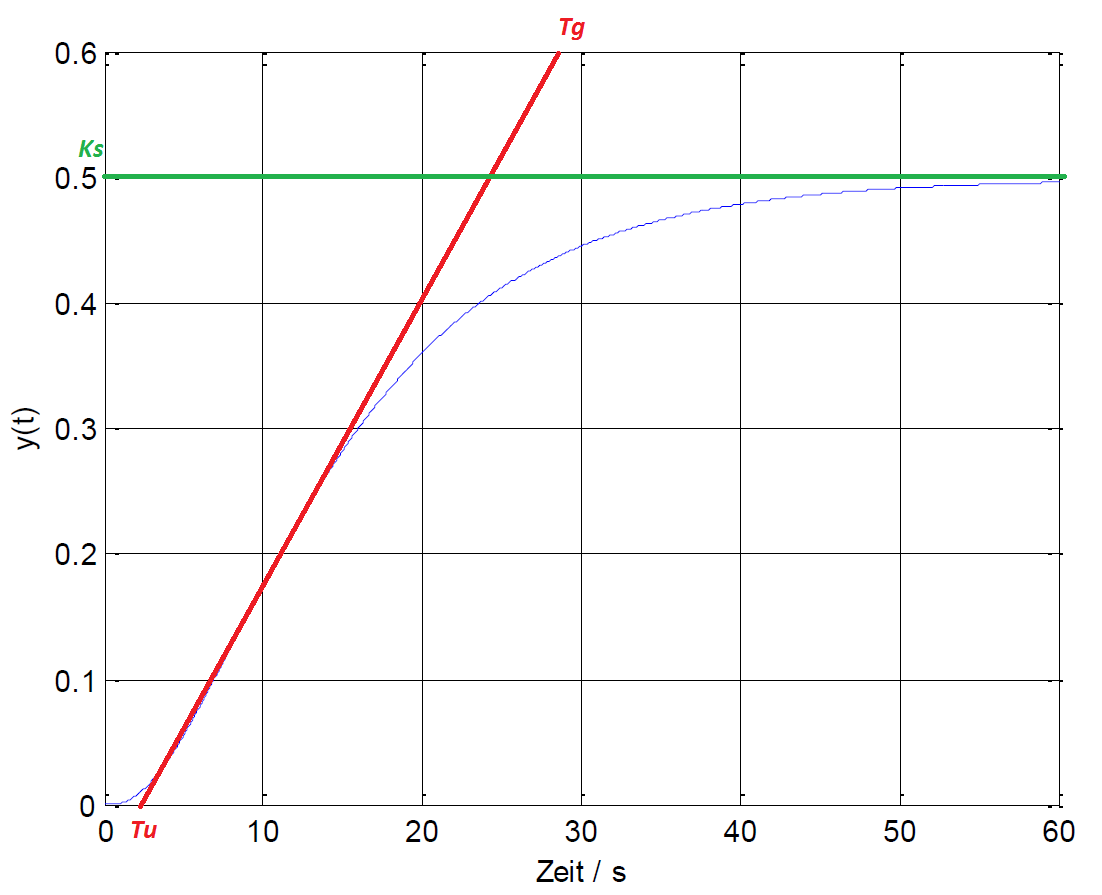
\includegraphics[width=0.5\textwidth]{./Wendetangente.png}
\caption{Regler und Regelstrecke\cite{WendetangenteAuftraggeber}}
\label{fig:Wendetangente}
\end{figure}

Mithilfe dieser Werte und der Sani Methode, welche vom Auftraggeber in Form eines Matlab-Files zur Verf�gung gestellt wurde, ist es einem nun m�glich, die Ordnung der Strecke sowie die Zeitkonstanten $T1$ bis $Tz$ zu berechnen, wobei $Z$ die Ordnung der Strecke ist. Diese Zeitkonstanten werden schlussendlich dazu verwendet die �bertragungsfunktion $H(s)$ zu berechnen:

\[
s=j\cdot w
\]

\begin{equation}\label{eq:�bertragungsfunktionStrecke}
H(s)=\prod\limits_{m=1}^Z \frac{1}{(1+s\cdot T_{m})}
\end{equation}

F�r die �bertragungsfunktion eines PI/PID Reglers gilt es zu beachten, dass es zwei Darstellungsarten gibt, die Reglerkonforme, sowie die Bodekonforme. Diese sehen wie folgt aus: \\


PI Reglerkonform:

\begin{equation}\label{eq:PITransmit}
G_{R}(s) = K_{R}\left(1+\frac{1}{s\cdot Tn}\right)
\end{equation}

PI Bodekonform:

\begin{equation}\label{eq:PITransmitBode}
G_{R}(s) = K_{R}\left(\frac{1+s\cdot Tn}{s\cdot Tn}\right)
\end{equation}

PID Reglerkonform:

\begin{equation}\label{eq:PIDTransmit}
G_{R}(s) = K_{R}\left(1+\frac{1}{s\cdot Tn}+\frac{s\cdot Tv}{1+s\cdot Tp}\right)
\end{equation}


PID Bodekonform:

\begin{equation}\label{eq:PIDTransmitBode}
G_{R}(s) = K_{RK}\left(\frac{(1+s\cdot Tnk)(1+s\cdot Tvk)}{s\cdot Tnk(1+s\cdot Tp)}\right)
\end{equation}

Auf die Verwendung dieser Funktionen sowie deren Herleitung wird im Kapitel \ref{ZellwegerMethode}, Zellweger Methode sowie auch im Anhang \ref{Bodekonf} genauer eingegangen.
%\end{document}

%\documentclass{fhnwreport} %
%\usepackage[ngerman]{babel}
%\usepackage[T1]{fontenc}
%\usepackage[latin1]{inputenc}
%\usepackage{tikz}
%\usepackage{amsmath}
%\usetikzlibrary{arrows}
%\usepackage{lmodern}   %Type1-Schriftart f�r nicht-englische Texte 
%
%\usepackage{listings}
%\lstset{language=Matlab}
%
%\usepackage{color}
%
%% Farben f�r Matlab-Listings
%\definecolor{hellgelb}{rgb}{1,1,0.85}     % Hintergrundfarbe
%\definecolor{colKeys}{RGB}{0,0,255}       % blau
%\definecolor{colIdentifier}{RGB}{0,0,0}	  % schwarz
%\definecolor{colComments}{RGB}{34,139,34} % gruen
%\definecolor{colString}{RGB}{160,32,240}  % violett
%
%\lstset{%
    %language=Matlab,%
    %%backgroundcolor={\color{hellgelb}},%
		%backgroundcolor={},%
    %basicstyle={\footnotesize\ttfamily},%
    %breakautoindent=true,%
    %breakindent=10pt,%
    %breaklines=true,%
    %captionpos=t,%
    %columns=fixed,%
    %%commentstyle={\itshape\color{colComments}},%
		%commentstyle={\color{colComments}},
    %extendedchars=true,%
    %float=hbp,%
    %frame=single,%
    %framerule=1pt,%
    %identifierstyle={\color{colIdentifier}},%
    %keywordstyle={\color{colKeys}},%
    %numbers=left,%
    %numbersep=1em,%
    %numberstyle={\tiny\ttfamily},%
    %showspaces=false,%
    %showstringspaces=false,%
    %stringstyle={\color{colString}},%
    %tabsize=4,%
    %xleftmargin=1em,%
    %xrightmargin=1em%
%} 
%
%
%\begin{document}

\subsection{Faustformeln}\label{FistFormula}

Zum Dimensionieren von verschiedenen Reglertypen gibt es eine Vielzahl von fixen Einstellregeln. Diese sind einfach anzuwenden, da sie keine besonderen Vorkenntnisse ben�tigen, jedoch ist deren Genauigkeit oftmals ungen�gend. Die f�r dieses Projekt relevanten Faustformeln sind:

\begin{itemize}
	\item Chien/Hrones und Reswick
	\item Oppelt
	\item Rosenberg
\end{itemize}

Diese Faustformeln wurden gew�hlt, da sie ebenfalls die Werte $Ks$, $Tu$ und $Tg$ verwenden, welche mittels Wendetangenten aus der Schrittantwort herausgelesen werden k�nnen, die uns vom Auftraggeber zur Verf�gung gestellt wurde.

Zur Verifizierung der Faustformeln wurden verschiedene Quellen verglichen und die Mehrheit wurde als richtig angesehen. %Quellenindex hinzuf�gen [3] [4] in Pflichtenheft

\subsubsection{Chien/Hrones und Reswick}
\paragraph{PI}
\begin{itemize}
	\item Aperiodischer Verlauf
	\begin{itemize}
		\item Gutes St�rverhalten
			
			\[
				Kr=0.6\cdot\frac{Tg}{Ks\cdot Tu}
			\]
						
			\[
				Tn=4\cdot Tu
			\]
			
			\item Gutes F�hrungsverhalten
			
			\[
				Kr=0.45\cdot\frac{Tg}{Ks\cdot Tu}
			\]
						
			\[
			Tn=1.2\cdot Tg
			\]
		
		\end{itemize}
	\item	20\% �berschwingen
		\begin{itemize}
			\item Gutes St�rverhalten
			
			\[
				Kr=0.7\cdot\frac{Tg}{Ks\cdot Tu}
			\]
			
			\[
			Tn=2.3\cdot Tu
			\]
			\item Gutes F�hrungsverhalten
			
			\[
				Kr=0.6\cdot\frac{Tg}{Ks\cdot Tu}
			\]
			
			\[
			Tn=Tg
			\]
		\end{itemize}
\end{itemize}
\paragraph{PID}
\begin{itemize}
	\item Aperiodischer Verlauf
	\begin{itemize}
		\item Gutes St�rverhalten
		\[
		Kr=0.95\cdot\frac{Tg}{Ks\cdot Tu}
		\]
		
		\[
		Tn=2.4\cdot Tu
		\]
		
		\[
		Tv=0.42\cdot Tu
		\]
		
		\item Gutes F�hrungsverhalten
		
		\[
		Kr=0.6\cdot\frac{Tg}{Ks\cdot Tu}
		\]
		
		\[
		Tn=Tg
		\]
		
		\[
		Tv=0.5\cdot Tu
		\]
		
	\end{itemize}
	\item 20\% �berschwingen
	\begin{itemize}
		\item Gutes St�rverhalten
		
		\[
		Kr=1.2\cdot\frac{Tg}{Ks\cdot Tu}
		\]
		
		\[
		Tn=2\cdot Tu
		\]
		
		\[
		Tv=0.42\cdot Tu
		\]
		
		\item Gutes F�hrungsverhalten
		
		\[
		Kr=0.95\cdot\frac{Tg}{Ks\cdot Tu}
		\]
		
		\[
		Tn=1.35\cdot Tg
		\]
		
		\[
		Tv=0.47\cdot Tu
		\]
		
	\end{itemize}
\end{itemize}

\subsubsection{Oppelt}
\paragraph{PI}
\[
Kr=0.8\cdot\frac{Tg}{Ks\cdot Tu}
\]

\[
Tn=3\cdot Tu		
\]
\paragraph{PID}

\[
Kr=1.2\cdot\frac{Tg}{Ks\cdot Tu}		
\]

\[
Tn=2\cdot Tu		
\]

\[
Tv=0.42\cdot Tu		
\]

\subsubsection{Rosenberg}
\paragraph{PI}

\[
Kr=0.91\cdot\frac{Tg}{Ks\cdot Tu}		
\]

\[
Tn=3.3\cdot Tu		
\]

\paragraph{PID}

\[
Kr=1.2\cdot\frac{Tg}{Ks\cdot Tu}
\]

\[
Tn=2\cdot Tu		
\]

\[
Tv=0.44\cdot Tu
\]
%\end{document}
%\documentclass{fhnwreport} %
%\usepackage[ngerman]{babel}
%\usepackage[T1]{fontenc}	
%\usepackage[latin1]{inputenc}
%\usepackage{tikz}
%\usepackage{amsmath}
%\usetikzlibrary{arrows}
%\usepackage{lmodern}   %Type1-Schriftart f�r nicht-englische Texte 
%\bibliographystyle{IEEEtran}
%
%\usepackage{listings}
%\lstset{language=Matlab}
%
%\usepackage{cite}
%\usepackage{hyperref}
%%\usepackage{url}
%\hypersetup{
     %colorlinks   = true,
     %urlcolor    = black
%}
%
%% Farben f�r Matlab-Listings
%\definecolor{hellgelb}{rgb}{1,1,0.85}     % Hintergrundfarbe
%\definecolor{colKeys}{RGB}{0,0,255}       % blau
%\definecolor{colIdentifier}{RGB}{0,0,0}	  % schwarz
%\definecolor{colComments}{RGB}{34,139,34} % gruen
%\definecolor{colString}{RGB}{160,32,240}  % violett
%
%\lstset{%
    %language=Matlab,%
    %%backgroundcolor={\color{hellgelb}},%
		%backgroundcolor={},%
    %basicstyle={\footnotesize\ttfamily},%
    %breakautoindent=true,%
    %breakindent=10pt,%
    %breaklines=true,%
    %captionpos=t,%
    %columns=fixed,%
    %%commentstyle={\itshape\color{colComments}},%
		%commentstyle={\color{colComments}},
    %extendedchars=true,%
    %float=hbp,%
    %frame=single,%
    %framerule=1pt,%
    %identifierstyle={\color{colIdentifier}},%
    %keywordstyle={\color{colKeys}},%
    %numbers=left,%
    %numbersep=1em,%
    %numberstyle={\tiny\ttfamily},%
    %showspaces=false,%
    %showstringspaces=false,%
    %stringstyle={\color{colString}},%
    %tabsize=4,%
    %xleftmargin=1em,%
    %xrightmargin=1em%
%} 
%\begin{document}
\subsection{Zellweger Methode}\label{ZellwegerMethode}


Der PI- oder PID-Regler wird aus dem Amplituden- und Phasengang mit der Phasengangmethode nach Zellweger berechnet. Der Amplituden- und 
Phasengang kann aus der �bertragungsfunktion $H(s)$ (Formel \eqref{eq:�bertragungsfunktionStrecke}) berechnet werden. 
Folgend werden die dazu verwendeten Formeln aufgef�hrt:

\[ %\label{Amplitudengang}
\text{Amplitudengang Strecke}~A_{s}(\omega)= Ks\cdot\prod\limits_{m=1}^Z\frac{1}{\sqrt{1+{(\omega\cdot T_{m})}^{2}}}
\]

\[ %\label{Phasengang}
\text{Phasengang Strecke}~\phi_{s}(\omega)=-1\cdot\sum\limits_{m=1}^Z\arctan \left( \omega\cdot T_{m}\right)
\]

Gem�ss Zellweger wird nun nach folgendem Rezept vorgegangen:

\textbf{1.} Aus dem Phasengang $\phi_{s}$ wird die Frequenz bei 
einem bestimmten Winkel $\phi_{x}$ herausgesucht. Der Winkel 
$\phi_{x}$ ist abh�ngig davon, welcher Regler-Typ 
dimensioniert werden soll. Beim PI-Regler ist $\phi_{pi}$ 
-90\textdegree, beim PID-Regler ist $\phi_{pid}$ -135\textdegree . 

Gem�ss dem Skript \glqq Regelkreise und Regelung\grqq\cite{Zellweger}
von Zellweger gibt es f�r die Regler zwei Darstellungsvarianten: Die reglerkonforme und die bodekonforme Darstellung.

Bei den weiteren Berechnungen des PID-Reglers muss f�r die 
Phasengang-Methode nach Zellweger in die bodekonforme Darstellung gewechselt werden (siehe Anhang Seite \pageref{Bodekonf} Kapitel \ref{Bodekonf}).

F�r PI- und PID-Regler unterscheidet sich nun das weitere Vorgehen. Es ist nun in die folgenden zwei Kapitel aufgeteilt.

\textbf{Weiteres Vorgehen PI Regler:}

Die gefundene Frequenz $\omega_{pi}$ bei $phi_{pi}$ 
entspricht $1/Tn$. 

\[
Tn=\frac{1}{\omega_{pi}}
\]

\textbf{2.} Mit dem gefundenen $Tn$ und $Kr=1$ wird der Amplituden- und 
Frequenzgang des offenen Regelkreises $(Go)$ berechnet. Das heisst Regler $(Gr)$ 
und Strecke $(Gs)$ in Serie, aber ohne R�ckkoppelung.\\

 
%\[
%\text{�bertragungsfunktion PI-Regler (Reglerkonform)}~Gr=Kr\cdot 
%\left[ 1+\frac{1}{s\cdot Tn} \right]
%\]
\begin{center}
�bertragungsfunktion PI-Regler (Reglerkonform) siehe Formel \eqref{eq:PITransmit}

%\[
%\text{�bertragungsfunktion PI-Regler (Bodekonform)}~Gr=Kr\cdot 
%\frac{1+s\cdot Tn}{s\cdot Tn}
%\]
�bertragungsfunktion PI-Regler (Bodekonform) siehe Formel \eqref{eq:PITransmitBode}
\end{center}

\[
\text{Phasengang PI-Regler}~\phi_{r}=\arctan \left( \omega\cdot Tn 
\right)-\frac{\pi}{2}
\]

\[
\text{Amplitudengang PI-Strecke}~A_{r}=\, Kr\frac{\sqrt {1+{(\omega\cdot 
Tn)}^{2}} }{\omega\cdot Tn}
\]


\[
\text{Phasengang Regelkreis offen}~\phi_{o}=\, 
\phi_{s}+\phi_{r}\, 
\]

\[
\text{Amplitudentang Regelkreis offen}~A_{ 
o}=A_{s}\cdot A_{r}
\]

\textbf{3.} Jetzt wird abh�ngig vom gew�nschten �berschwingen 
des Reglers ein Winkel auf dem Phasengang des offenen Regelkreises gesucht. 
Folgende Tabelle zeigt den Zusammenhang des f�r die Dimensionierung 
gew�hlten �berschwingens und des dazu geh�rigen Winkels.

\begin{table}[h]

\centering
	\begin{tabular}{|p{106pt}|r|r|r|}
	\hline
	D�mpfmass d & $\phi_{rand}$ & $\phi_{st}$ & �berschwingen \\
	\hline
	0.42 & 45\textdegree & -135\textdegree & 23.3\% \\
	\hline
	0.5 & 51.5\textdegree & -128.5\textdegree & 16.3\% \\
	\hline
	0.7 & 65.5\textdegree & -114.6\textdegree & 4.6\% \\
	\hline
	1 & 76.3\textdegree & -103.7\textdegree & 0\% \\
	\hline
	\end{tabular}
	\caption{Phasenwinkel abh�ngig vom gew�nschten �berschwingen}
	\label{table:Tab�berschwingen}
\end{table}


Bei 0\% �berschwingen muss beispielsweise der Winkel $\phi_{st}$ 
gleich -103.7\textdegree ~auf dem Phasengang gesucht werden. Bei der 
gefundenen Frequenz wird der dazu geh�rige Wert aus dem Amplitudengang 
des offenen Regelkreises herausgelesen. Um diesen Faktor muss die 
Verst�rkung des Reglers vermindert werden. Der aus dem Amplitudengang 
herausgelesene Wert mit (-1) multipliziert ergibt also den Regler-Parameter 
$Kr$.\\

\textbf{Weiteres Vorgehen PID Regler:}

Beim PID-Regler wird analog zum beim PI-Regler beschriebenen Vorgehen 
gerechnet. Die gefundene Frequenz $\omega_{pid}$ f�r $\phi_{pid}$ 
$=$ -135\textdegree ~entspricht aber nicht direkt $1/Tn$ wie beim PI-Regler.

Die Zellweger'sche Phasengang-Methode berechnet beim PID-Regler $Tnk$, $Tvk$ und 
$Krk$. Dies sind Parameter in der bodekonformen Darstellung. Diese Parameter 
k�nnen schliesslich wieder in die Parameter $Tn$, $Tv$ und $Kr$ der 
reglerkonformen Darstellung umgerechnet werden.

\textbf{2.} F�r die Berechnung von $Tnk$ und $Tvk$ wird ein Parameter $\beta$ 
ben�tigt. Folgend wird die Berechnung davon aufgef�hrt:

\[
\frac{2\cdot \beta}{1+\beta^{2}}-w_{PID} \cdot  \sum \limits_{m=1}^{n} \frac{T_m}{1+ (w_{PID} \cdot T_m)^2} =-0.5
\]

Folgendes wird mit $Z$ substitutiert:

\[
Z=\frac{2\cdot \beta}{1+\beta^{2}}
\]

\[
Z=w_{PID} \cdot  \sum \limits_{m=1}^{n} \frac{T_m}{1+ (w_{PID} \cdot T_m)^2} -0.5
\]

$\beta$ kann nun durch folgende Gleichung beschrieben werden:

\[
\beta = \frac{1}{Z} - \sqrt{\frac{1}{Z^2}-1}
\]

$\beta$ muss zwischen 0 und 1 liegen. Damit es keine komplexen L�sungen 
gibt, wird $\beta$ f�r $Z$ \textgreater 1 gleich 1. F�r eine detaillierte Herleitung von $\beta$ siehe Anhang \ref{ZellwegerBeta}.

\textbf{3.} $Tnk$ und $Tvk$ k�nnen nun wie folgt mit $\beta$ berechnet werden:

\[
\frac{1}{Tnk}=\omega_{pid}\cdot \beta
\]

\[
\frac{1}{Tvk}=\frac{\omega_{pid}}{\beta}
\]

\textbf{4. }F�r die Berechnung des D�mpfungsfaktors $Krk$ muss beim 
PID-Regler folglich die Formel der �bertragungsfunktion \eqref{eq:�bertragungsfunktionStrecke} des PID-Reglers 
verwendet werden. Der Regler-Parameter $Tp$ wird ben�tigt, weil der Regler 
nicht �ber eine unendlich kurze Zeit differenzieren kann. $1/Tp$ muss ca. 
1 Dekade h�her als $1/Tvk$ gew�hlt werden. Beim PID-Regler wird die 
Bodekonforme Darstellung verwendet, weil $Tnk$ und $Tvk$ vorhanden sind, $Tn$ und $Tk$ jedoch noch nicht. Eine genauere Erl�ueterung dieser ist im Anhang Seite \pageref{Bodekonf} Kapitel \ref{Bodekonf} zu finden. F�r die Berechnung des Amplitudenganges wird $Krk=1$ verwendet: 

\[
\frac{1}{Tp}=10\cdot \frac{1}{Tnk}
\]\\


\begin{center}
%\[
%\text{�bertragungsfunktion PID-Regler (Reglerkonform)}~Gr=Kr\cdot \left[ 
%1+\frac{1}{s\cdot Tn}+\frac{s\cdot Tv}{1+s\cdot Tp} \right]
%\]
�bertragungsfunktion PID-Regler (Reglerkonform) siehe Formel \eqref{eq:PIDTransmit}

%\[
%\text{�bertragungsfunktion PID-Regler (Bodekonform)}~Gr=Krk\cdot \left[ 
%\frac{\left( 1+s\cdot Tnk \right)\cdot (1+s\cdot Tvk)}{s\cdot Tnk\cdot (1+s\cdot 
%Tp)} \right]
%\]
�bertragungsfunktion PID-Regler (Bodekonform) siehe Formel \eqref{eq:PIDTransmitBode}
\end{center}

\[
\text{Phasengang PID-Regler}~\phi_{r}=\arctan {\left( \omega\cdot Tnk 
\right)+arctan\left(\omega\cdot Tvk \right)-\mathrm{arctan}(\omega\cdot 
Tp)}-\frac{\pi}{2}
\]

\[
\text{Amplitudengang PID-Regler}~A_{r}=\, Krk\frac{\sqrt {1+\left( 
\omega\cdot Tnk \right)^{2}} \cdot \sqrt {1+{(\omega\cdot Tvk)}^{2}} }{\omega\cdot Tnk}
\]

\[
\text{Phasengang Regelkreis offen}~\phi_{o}=\, 
\phi_{s}+\phi_{r}\, 
\]

\[
\text{Amplitudentang Regelkreis offen}~A_{ 
o}=A_{s}\cdot A_{r}
\]

\textbf{5.} Abh�ngig vom gew�hlten �berschwingen wird wiederum ein Winkel auf dem Phasengang $\phi_{o}$ gesucht (Siehe Tabelle \ref{table:Tab�berschwingen} Seite \pageref{table:Tab�berschwingen}). Die Amplitude bei diesem Winkel mit (-1) multipliziert ergibt $Krk$.

%\end{document}
%\documentclass{fhnwreport} %
%\usepackage[ngerman]{babel}
%\usepackage[T1]{fontenc}
%\usepackage[latin1]{inputenc}
%\usepackage{tikz}
%\usepackage{amsmath}
%\usetikzlibrary{arrows}
%\usepackage{lmodern}   %Type1-Schriftart f�r nicht-englische Texte 
%\usepackage{graphicx}
%\usepackage{listings}
%\lstset{language=Matlab}
%
%\usepackage{color}
%
%% Farben f�r Matlab-Listings
%\definecolor{hellgelb}{rgb}{1,1,0.85}     % Hintergrundfarbe
%\definecolor{colKeys}{RGB}{0,0,255}       % blau
%\definecolor{colIdentifier}{RGB}{0,0,0}	  % schwarz
%\definecolor{colComments}{RGB}{34,139,34} % gruen
%\definecolor{colString}{RGB}{160,32,240}  % violett
%
%\lstset{%
    %language=Matlab,%
    %%backgroundcolor={\color{hellgelb}},%
		%backgroundcolor={},%
    %basicstyle={\footnotesize\ttfamily},%
    %breakautoindent=true,%
    %breakindent=10pt,%
    %breaklines=true,%
    %captionpos=t,%
    %columns=fixed,%
    %%commentstyle={\itshape\color{colComments}},%
		%commentstyle={\color{colComments}},
    %extendedchars=true,%
    %float=hbp,%
    %frame=single,%
    %framerule=1pt,%
    %identifierstyle={\color{colIdentifier}},%
    %keywordstyle={\color{colKeys}},%
    %numbers=left,%
    %numbersep=1em,%
    %numberstyle={\tiny\ttfamily},%
    %showspaces=false,%
    %showstringspaces=false,%
    %stringstyle={\color{colString}},%
    %tabsize=4,%
    %xleftmargin=1em,%
    %xrightmargin=1em%
%} 
%\graphicspath{{./PrettyPictures/}}
%
%\begin{document}
\subsubsection{Numerisches Beispiel PI-Regler}\label{PIExample}
Im folgenden Abschnitt wird ein Berechnungsbeispiel zum PI-Regler durchgef�hrt. Folgende Werte werden verwendet:

$Ks$ = 0.5\\
$Tu$ = 2.5\\
$Tg$ = 18.3\\
$\phi_{Strecke}$ = -114.6\textdegree (entspricht 4,6\% �berschwingen)\\

Zun�chst werden die Zeitkonstanten sowie die Ordnung der Strecke  mithilfe der Sani Methode bestimmt. Bei unserer Strecke ergibt dies eine Strecke 3.Ordnung und die folgenden Zeitkonstanten:

$T1=1.0688s$\\
\\
$T2=3.3484s$\\
\\
$T3=10.4901s$\\
\\
Nun wird der Frequenzgang aus der �bertragungsfunktion \eqref{eq:�bertragungsfunktionStrecke} berechnet und in einem Plot aufgezeichnet (siehe Abbildung \ref{fig:PIStep1}). Danach wird der -90\textdegree ~Punkt auf dem Phasengang gesucht (mit blau gestrichelter Linie in Abbildung \ref{fig:PIStep1} dargestellt). Dies ergibt eine Frequenz $\omega_{PI}$ von $0.1415s^{-1}$. Daraus berechnet sich die Zeitkonstante $Tn=7.0647s$.

\begin{figure}[h]	
\centering		
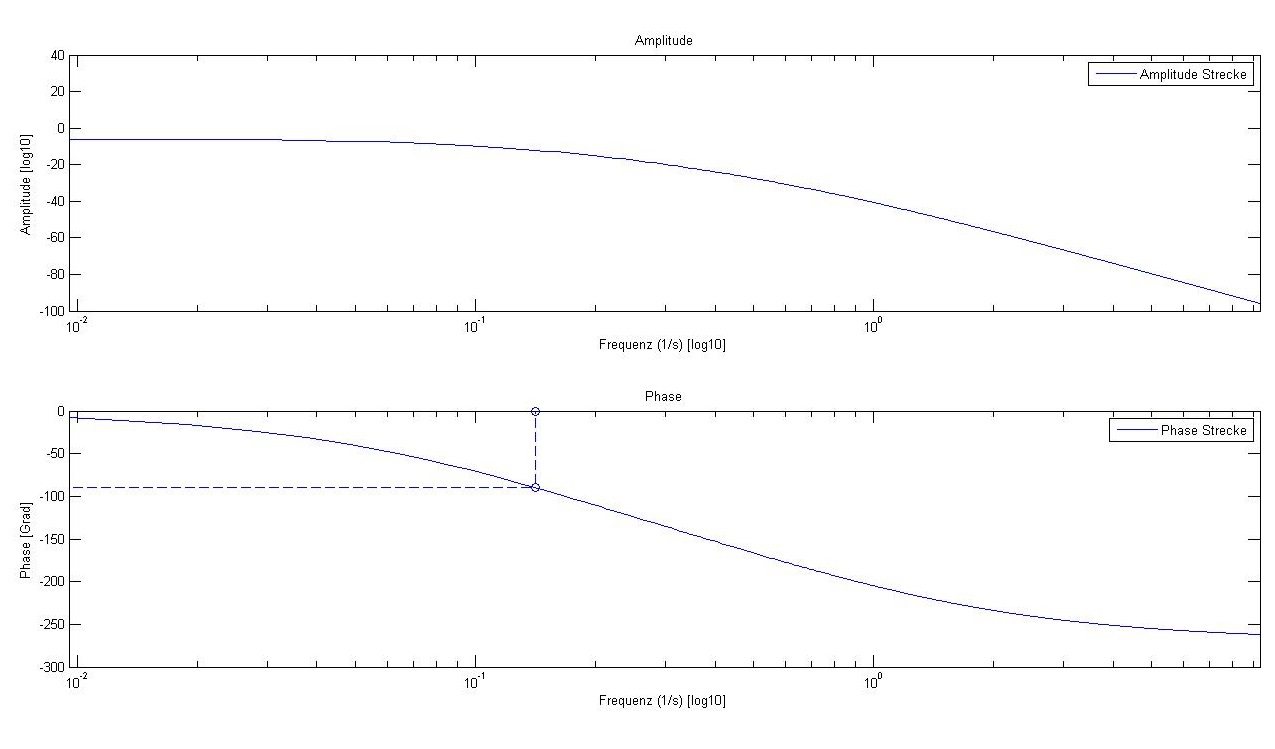
\includegraphics[width=1.0\textwidth]{PI_Step_01.jpg}
\caption{Amplituden- und Phasengang der Regelstrecke}	
\label{fig:PIStep1}	
\end{figure}

\newpage
Im n�chsten Schritt berechnet man mithilfe von $Tn$ und mit $Kr=1$ den offenen Regelkreis (rot dargestellt in Abbildung \ref{fig:PIStep2}).


\begin{figure}[h]	
\centering		
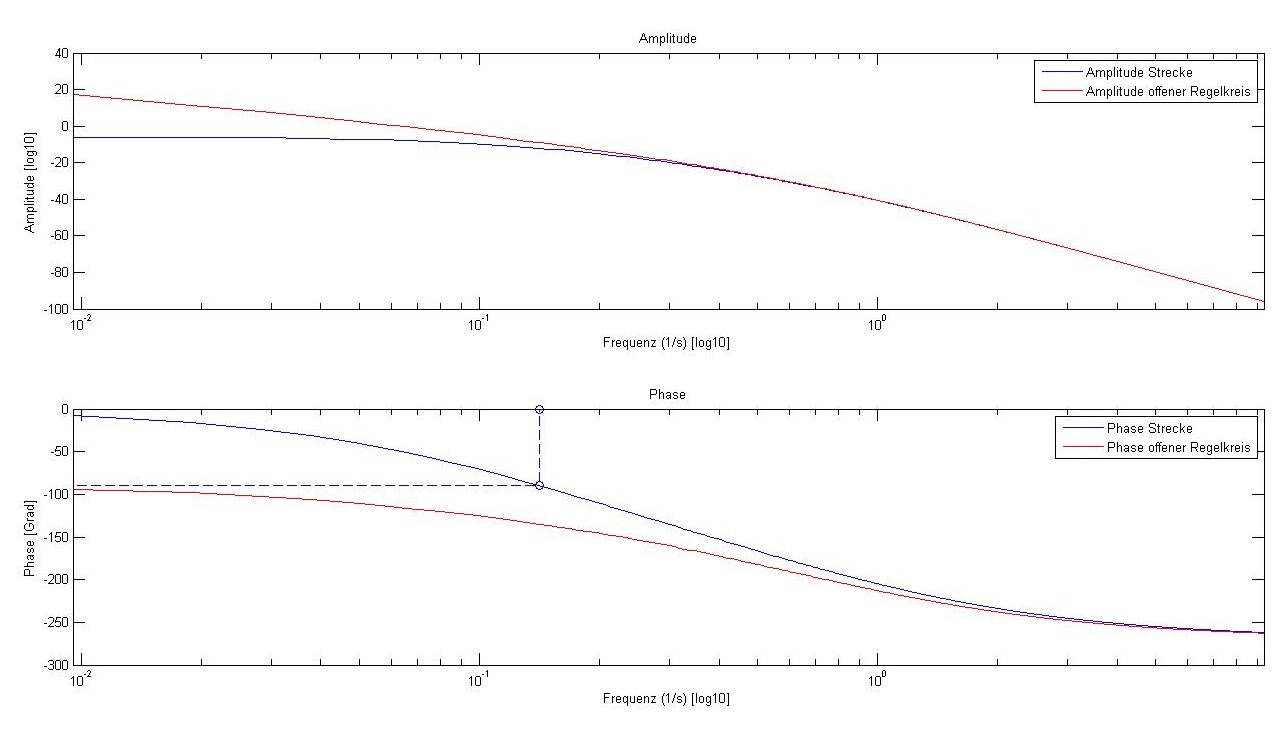
\includegraphics[width=1.0\textwidth]{PI_Step_02.jpg}
\caption{Frequenzgang der offenen Strecke}
\label{fig:PIStep2}
\end{figure}

Auf dem Phasengang des offenen Regelkreises (Abbildung \ref{fig:PIStep3}) wird nun die Frequenz bei $\phi_{Strecke}$ mithilfe der Tabelle \ref{table:Tab�berschwingen} auf Seite \pageref{table:Tab�berschwingen} gesucht (rot gestrichelte Linie). Die gefundene Frequenz ist $0.0611s^{-1}$.

\begin{figure}[h!]	
\centering		
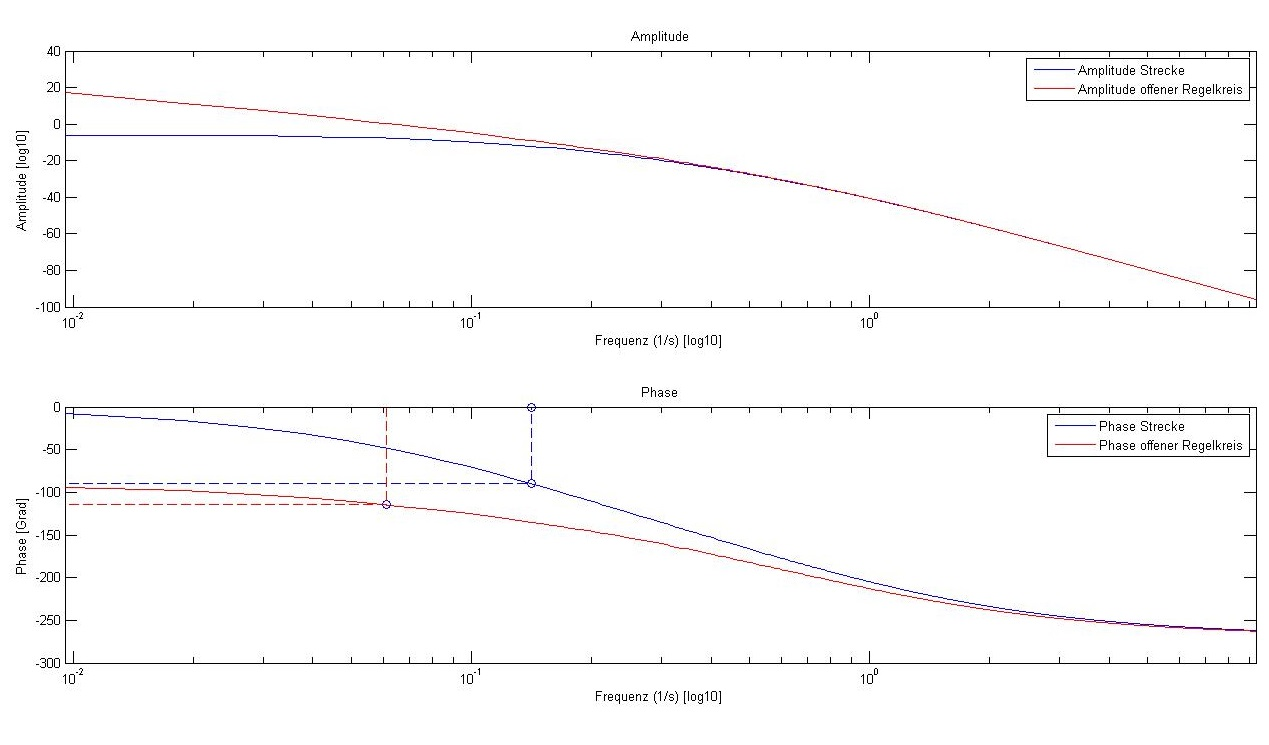
\includegraphics[width=1.0\textwidth]{PI_Step_03.jpg}
\caption{$\omega$ bei $\phi_{Strecke}$}	
\label{fig:PIStep3}	
\end{figure}

\newpage
Schliesslich wird die entsprechende Verst�rkung zur gefundenen Frequenz aus dem Amplitudengang des offenen Regelkreises herausgelesen (Abbildung \ref{fig:PIStep4}). In unserem Beispiel ergibt dies eine Verst�rkung von 1.0390.  Um diesen Faktor wird die Verst�rkung des Reglers gemindert, dies ergibt den letzten ben�tigten Parameter $Kr$.

\begin{figure}[h]	
\centering	
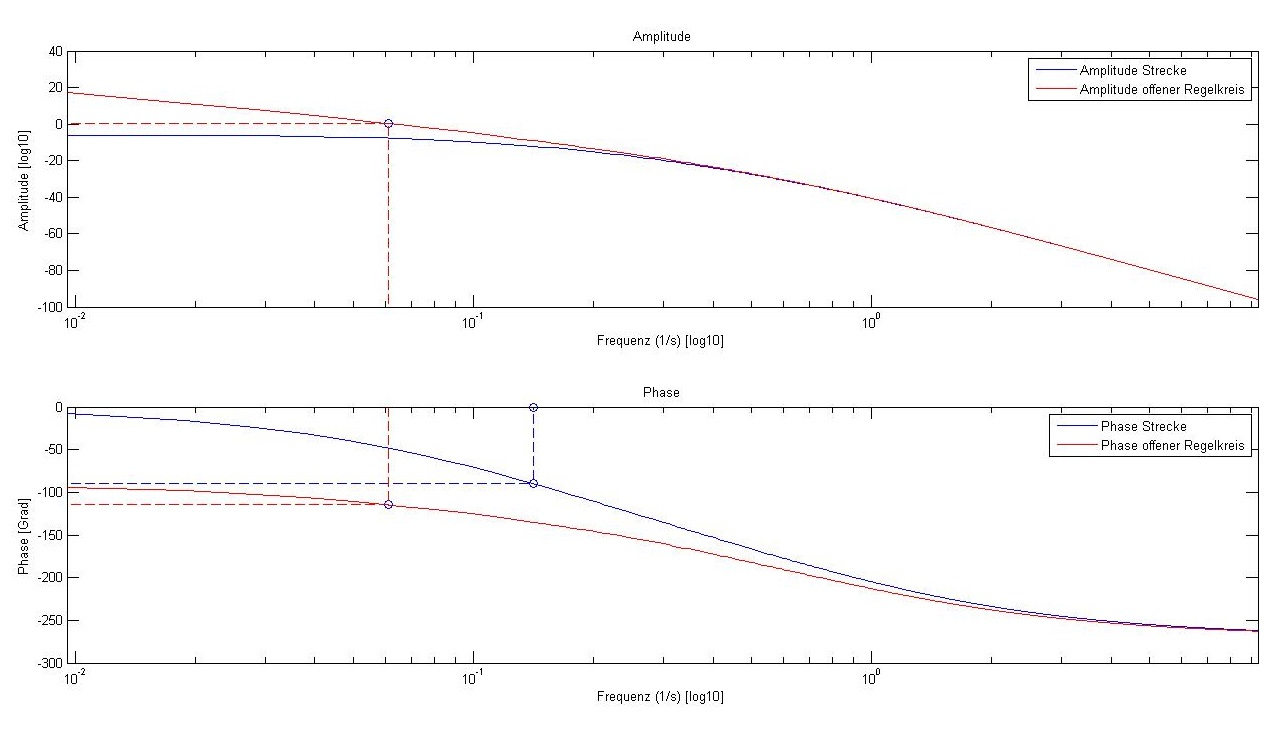
\includegraphics[width=1.0\textwidth]{PI_Step_04.jpg}
\caption{Bestimmung von $Kr$}	
\label{fig:PIStep4}	
\end{figure}

Die Endresultate dieser Berechnung sind:

$Tn = 7.0647s$\\
$Kr = 0.9625$

%\end{document}
%\documentclass{fhnwreport} %
%\usepackage[ngerman]{babel}
%\usepackage[T1]{fontenc}
%\usepackage[latin1]{inputenc}
%\usepackage{tikz}
%\usepackage{amsmath}
%\usetikzlibrary{arrows}
%\usepackage{lmodern}   %Type1-Schriftart f�r nicht-englische Texte 
%
%\usepackage{listings}
%\lstset{language=Matlab}
%
%\usepackage{color}
%
%% Farben f�r Matlab-Listings
%\definecolor{hellgelb}{rgb}{1,1,0.85}     % Hintergrundfarbe
%\definecolor{colKeys}{RGB}{0,0,255}       % blau
%\definecolor{colIdentifier}{RGB}{0,0,0}	  % schwarz
%\definecolor{colComments}{RGB}{34,139,34} % gruen
%\definecolor{colString}{RGB}{160,32,240}  % violett
%
%\lstset{%
    %language=Matlab,%
    %%backgroundcolor={\color{hellgelb}},%
		%backgroundcolor={},%
    %basicstyle={\footnotesize\ttfamily},%
    %breakautoindent=true,%
    %breakindent=10pt,%
    %breaklines=true,%
    %captionpos=t,%
    %columns=fixed,%
    %%commentstyle={\itshape\color{colComments}},%
		%commentstyle={\color{colComments}},
    %extendedchars=true,%
    %float=hbp,%
    %frame=single,%
    %framerule=1pt,%
    %identifierstyle={\color{colIdentifier}},%
    %keywordstyle={\color{colKeys}},%
    %numbers=left,%
    %numbersep=1em,%
    %numberstyle={\tiny\ttfamily},%
    %showspaces=false,%
    %showstringspaces=false,%
    %stringstyle={\color{colString}},%
    %tabsize=4,%
    %xleftmargin=1em,%
    %xrightmargin=1em%
%} 
%\graphicspath{{./PrettyPictures/}}
%
%\begin{document}
\subsubsection{Numerisches Beispiel PID-Regler }\label{PIDExample}
Die Berechnung eines PID-Reglers verl�uft �hnlich wie die eines PI-Reglers. F�r das Beispiel werden die gleichen Eingabeparameter verwendet wie beim PI-Regler:

$Ks=0.5$\\
$Tu=2.5$\\
$Tg=18.3$\\
$\phi_{Strecke}$=-114.6\textdegree\\

Im Gegensatz zum PI-Regler sind alle Ausgabeparameter in der bodekonformen Darstellung. Eine genauere Erkl�rung dazu ist im Anhang, Sektor \ref{Bodekonf}, Seite \pageref{Bodekonf} zu finden.

Zun�chst werden nun die Zeitkonstanten sowie die Ordnung der Strecke  mithilfe der Sani Methode bestimmt. Bei unserer Strecke ergibt dies eine Strecke 3. Ordnung und die folgenden Zeitkonstanten:

$T1=1.0688s$\\
\\
$T2=3.3484s$\\
\\
$T3=10.4901s$\\
\\
Nun wird der Frequenzgang aus der �bertragungsfunktion der Strecke \eqref{eq:�bertragungsfunktionStrecke} berechnet und in einem Plot aufgezeichnet (siehe Abbildung \ref{fig:PIDStep1}). Danach wird nach dem -135\textdegree ~Punkt auf dem Phasengang gesucht. Dieser ist mit der horizontalen blau gestrichelten Linie eingezeichnet und ergibt folgende Frequenz: $0.2987s^{-1}$.

\begin{figure}[h]	
\centering		
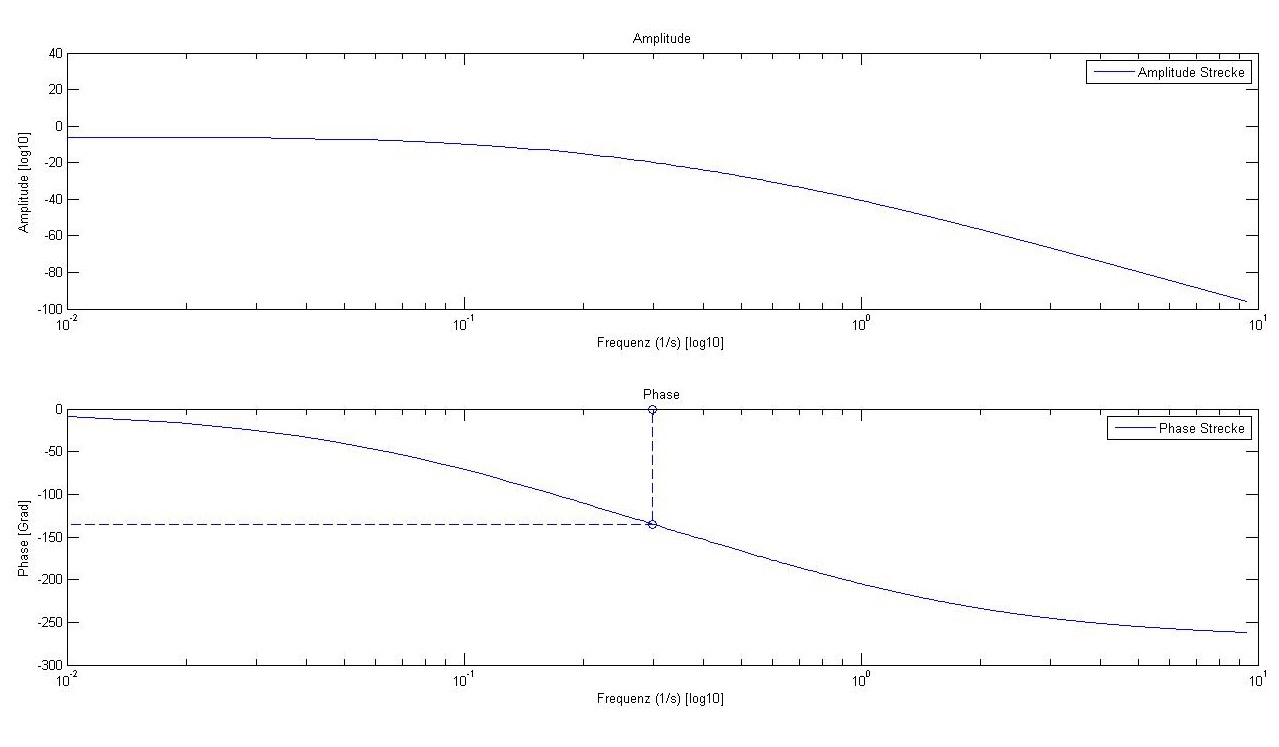
\includegraphics[width=1.0\textwidth]{PID_Step_01.jpg}
\caption{Amplituden- und Phasengang der Regelstrecke}	
\label{fig:PIDStep1}	
\end{figure}

\newpage
Bevor der Frequenzgang des offenen Regelkreises berechnet wird, muss $\beta$ bestimmt werden. Die Berechnung dazu ist im Anhang, Kapitel \ref{ZellwegerBeta} auf Seite \pageref{ZellwegerBeta} ersichtlich. Nach Ausf�hren dieser Berechnung erh�lt man $\beta=0.3192$.

Mit $\beta$ ist es m�glich, $Tnk=10.4902s$ und $Tvk=1.0688s$ zu berechnen.
Weiter wird noch $Tp$ bestimmt (siehe Kapitel \ref{ZellwegerMethode}, Seite \pageref{ZellwegerMethode}). In diesem Beispiel wurde $Tp$ eine Dekade kleiner als $Tvk$ gew�hlt, folglich ist der Wert von $Tp=0.107s$. 
Mit diesen Werten und $Krk =1$ wird nun der offene Amplituden- und Phasengang berechnet (Abbildung \ref{fig:PIDStep2}).

\begin{figure}[h]	
\centering		
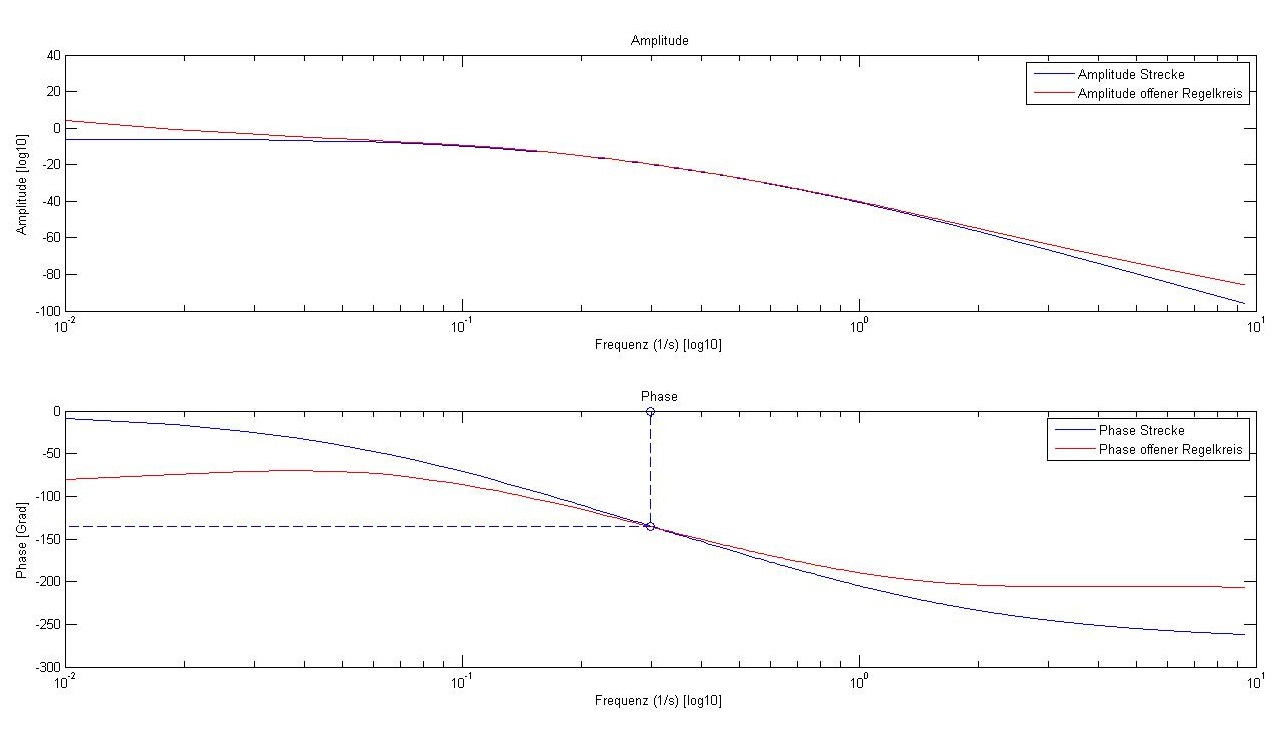
\includegraphics[width=1.0\textwidth]{PID_Step_02.jpg}
\caption{Frequenzgang der offenen Regelstrecke}	
\label{fig:PIDStep2}	
\end{figure}

%\newpage
Als n�chster Schritt wird die Tabelle \ref{table:Tab�berschwingen} auf Seite \pageref{table:Tab�berschwingen} zu Hilfe genommen. Daraus wird das gew�nschte �berschwingen ausgew�hlt und die entsprechende Frequenz auf dem Phasengang des offenen Regelkreises gesucht (siehe Abbildung \ref{fig:PIDStep3}). Die gefundene Frequenz lautet: $0.1317s^{-1}$.

\begin{figure}[h!]	
\centering		
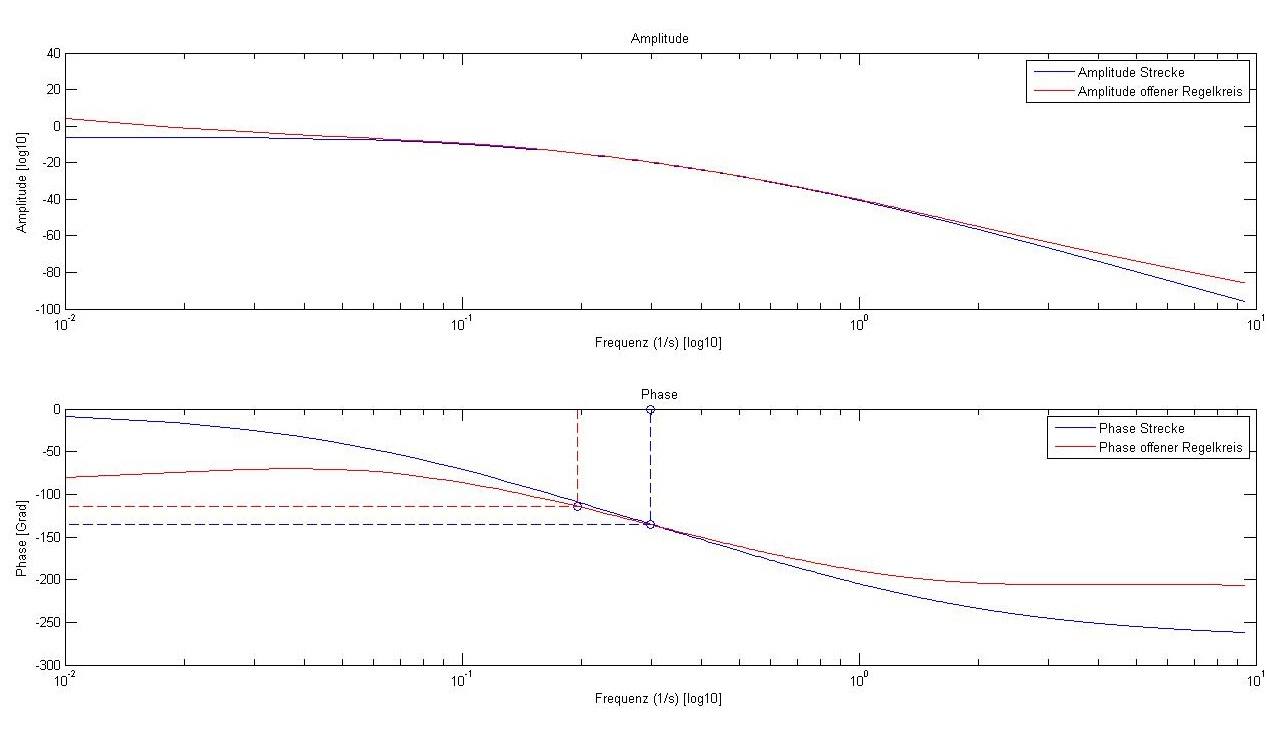
\includegraphics[width=1.0\textwidth]{PID_Step_03.jpg}
\caption{$\omega$ bei $\phi_{Strecke}$}	
\label{fig:PIDStep3}	
\end{figure}

\newpage
Zur gefundenen Frequenz liest man die Verst�rkung von $0.3312$ heraus. Der Kehrwert davon ergibt den letzten Faktor $Krk=3.0194$. (Abbildung \ref{fig:PIDStep4})

\begin{figure}[h!]	
\centering		
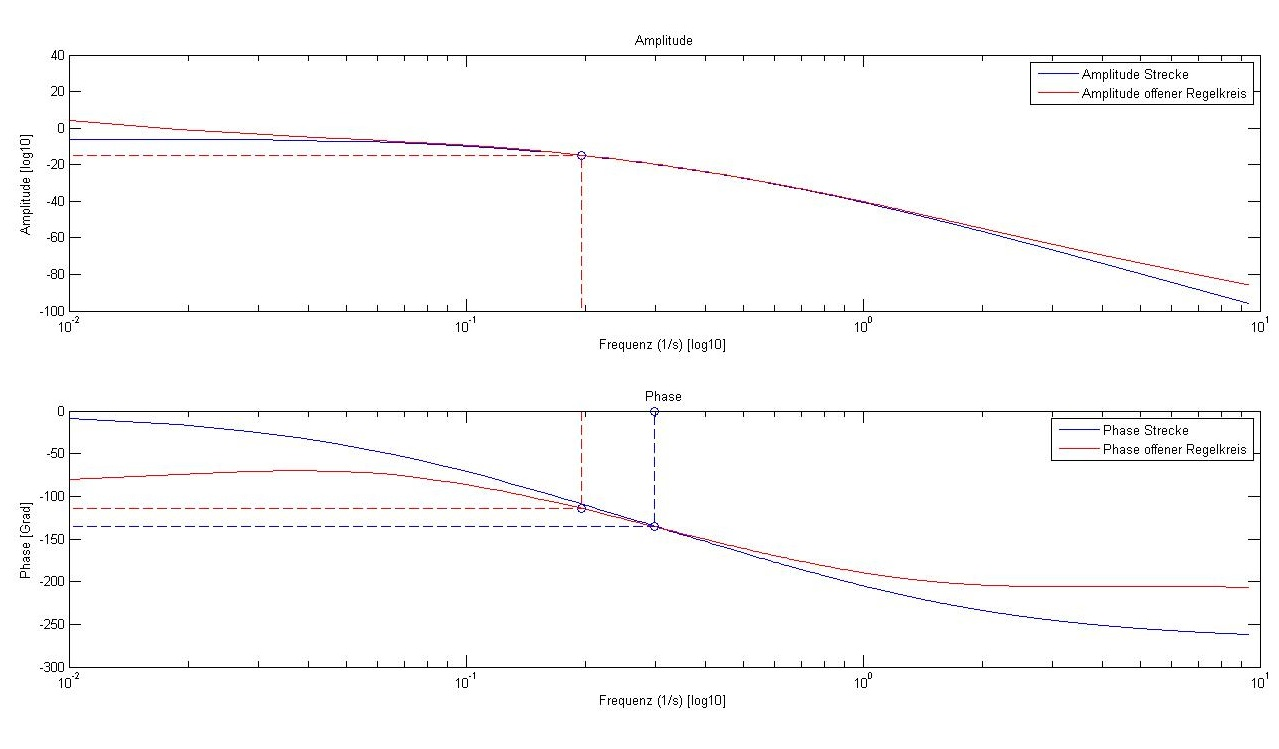
\includegraphics[width=1.0\textwidth]{PID_Step_04.jpg}
\caption{Bestimmung von $Krk$}	
\label{fig:PIDStep4}	
\end{figure}

\pagebreak
Die Endresultate dieser Berechnung sind:

$Tnk$ = 10.4902\\
$Tvk$ = 1.0688\\
$Krk$ = 3.0194

Wie schon erw�hnt, sind diese Angaben alle in der bodekonformen Darstellung. Umgewandelt in die reglerkonforme Darstellung ergibt dies folgende Werte:

$Tn =11.4521$\\
$Tv =0.8721$\\
$Kr =3.2963$

Den genauen Verlauf f�r die Umrechnung zur reglerkonformen Darstellung ist im Anhang, Sektor \ref{Bodekonf}, Seite \pageref{Bodekonf} zu finden.
	
%\end{document}


\section{Software}

Im folgenden Abschnitt wird der Aufbau der Software beschrieben. Die Software basiert auf dem Model-View-Controller Entwurfsmuster, welches f�r GUI-Applikationen aufgrund seiner hohen Flexibilit�t und Wiederverwendbarkeit als Standard gilt. Das Model-View-Controller Prinzip basiert auf den drei Hauptklassen \textit{Model}, \textit{View} und \textit{Controller}, welche kurz erl�utert werden:

\textbf{Model:} Das \textit{Model} enth�lt die Daten und Berechnungsmethoden, welche f�r die Software ben�tigt werden. Diese Daten sind unabh�ngig von der grafischen Darstellung der Software. Falls Daten im \textit{Model} ge�ndert werden, informiert das \textit{Model} die Klasse \textit{View}, welche die Daten f�r den Benutzer darstellt. \\
\textbf{View:} Die \textit{View} beinhaltet und visualisiert die Benutzeroberfl�che. Sie erh�lt dazu die Daten der Klasse \textit{Model}, welche grafisch dargestellt werden und leitet Eingaben an die Klasse \textit{Controller} weiter. In der Klasse \textit{View} werden keine Berechnungen durchgef�hrt. Das Model ist mit der \textit{View} mittels Observable-Observer Entwurfsmuster verkn�pft, wobei das \textit{Model} als Observable und die \textit{View} als Observer agiert.\\
\textbf{Controller:} Der \textit{Controller} �berpr�ft die Benutzereingaben und leitet diese, falls sie korrekt sind, zur weiteren Berechnung an das \textit{Model} weiter.

Im folgenden werden wiederholt Ausschnitte des Klassendiagramms gezeigt, das komplette Klassendiagramm findet sich im Anhang \ref{klassendiagramm}.


%\subsection{Beschreibung eines Benutzungsfalls (Use-Case)}
%
%Unsere Reise beginnt in der Klasse \em{InputPanel} - ein Attribut der Klasse \em{View} - mit drei Eingabefelder, die den Benutzer erlauben, die Strecke anhand der drei Parameter $T_u$, $T_g$ und $K_r$ zu beschreiben.
%
%Ist die Strecke beschrieben, so kann der Benutzer mit einer Drop-Down-Menu den gew�nschten Regler selektieren. Zur Auswahl stehen \em{I}, \em{PI}, und \em{PID} zur Verf�gung.
%
%Jenachdem welchen Regler der Benutzer ausw�hlt, kann er weiter das gew�nschte �berschwingen in Prozent eingeben und eine Parasit�re Zeitkonstantenfaktor definieren, welches zur Berechnung von $T_p$ gebraucht wird.
%
%Ist alles in Ordnung, so klickt der Benutzer auf den Button ``Simulieren'' und die erste Simulation wird initiiert.
%
%Die \em{View} nimmt die Eingabewerte des Benutzers und saniert sie, damit ung�ltige Einstellungen m�glichst fr�h erkannt werden. Ist alles saniert, so werden die Werte an der Klasse \em{Controller} mittels der Methode \em{Controller::btSimulateAction()} �bergeben.
%
%Der \em{Controller} konfiguriert das \em{Model}-Objekt mit den Eingabewerten mittels der Methoden \em{Model::setRegulatorType()} - welche den Typ zu \em{I}, \em{PI} oder \em{PID} setzt - \em{Model::setPlant()} - welche einen neuen \em{Plant}-Objekt erstellt und als Attribut der Klasse \em{Model} speichert - \em{Model::setParasiticTimeConstantFactor()}, und \em{Model::setOvershoot()}. Danach ruft sie die Methode \em{Model::simulateAll()} auf, um die Simulation zu beginnen.
%
%Das \em{Model} baut sich zuerst mit Hilfe seiner \em{Plant}-Objekt - welche die vom Benutzer eingegebene Strecke beschreibt - eine Liste von \em{CalculationCycle}-Objekten. Diese Objekte sind dazu f�hig, eine gesamte Berechnung von Reglerberechnung bis zur Schrittantwort durchzuf�hren. Welche Regler ausgerechnet werden ist abh�ngig vom Auswahl des Reglertyps, also \em{I}, \em{PI} oder \em{PID}.
%
%Es wird mittels \em{Model::notifySimulationBegin()} an alle Listener mitgeteilt, dass eine Simulation beginnt. Dies bewirkt unter anderem dass sich die verschiedene Panels auf die Resultate vorbereiten k�nnen, wie zum beispiel die Tabelle l�schen oder den Plot l�schen.
%
%Die \em{CalculationCycle}-Klasse erbt von \em{Runnable}. Es wird ein \em{ThreadPool} erstellt und alle \em{CalculationCycle}-Objekte werden parallel ausgef�hrt. Das Programm wartet, bis alle Berechnungen vollendet sind.
%
%Zu diesem Zeitpunkt teilt sich der Programmfluss in einer Unmenge kleiner Teilchen auf. Wir verfolgen nur einen Pfad, n�mlich die Berechnung eines PID-Reglers mittels Zellweger Methode.
%
%Beim Instanziieren der Klasse \em{CalculationCycle} wird ein \em{AbstractControllerCalculator} �bergeben - in diesem Fall ein Objekt, dass als Konkrete Klasse den \em{ZellwegerPID} hat. Dieses Objekt wurde schon vom \em{Model} konfiguriert, und es muss nur \em{AbstractControllerCalculator::run()} aufgerufen werden, um einen passenden Regler f�r die vom Benutzer definierte Strecke zu berechnen. 
%
%Die \em{run()}-Methode f�hrt dazu, dass die Methode \em{ZellwegerPID::calculate()} ausgef�hrt wird. Der implementierte Algorithmus von Herrn Zellweger wird in dieser Methode gebraucht, um ein neues \em{ControllerPID}-Objekt zu erstellen.

\subsection{Model}

Das \textit{Model} ist das Herzst�ck s�mtlicher Berechnungen. Dazu f�hrt es folgende Funktionen aus:

\begin{itemize}
	\item Die Koordination der unabh�ngigen und parallel verlaufenden Berechnungen der Reglertypen und deren Schrittantworten.
	\item Das Verwalten der dazu notwendigen Objekte, beispielsweise die Sani-Kurven.
	\item Die Implementation des iterativen Approximationsverfahren zur genauen Bestimmung des �berschwingens.
\end{itemize}

%Das Model ist das Herzst�ck aller Berechnungen. Es koordiniert die unabh�ngigen, parallel
%verlaufenden Berechnungen der Reglertypen wie auch deren Schrittantworten, es verwaltet
%die dazu notwendigen Objekte wie zum Beispiel die Sani-Kurven und es implementiert das
%iterative Approximationsverfahren zur genauen Bestimmung des �berschwingens.

\begin{figure}[h]
	\centering
		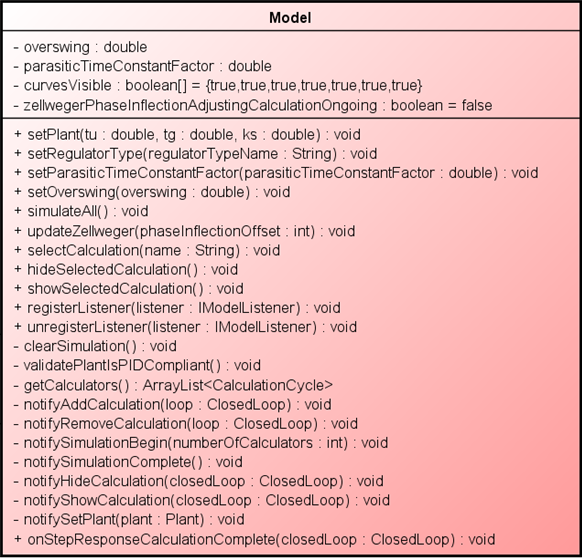
\includegraphics[width=0.60\textwidth]{model.png}
	\caption{Klassendiagramm des Models}
	\label{fig:model}
\end{figure}

\newpage
Als erstes wird die zu Grunde liegende Terminologie erl�utert:

Unter einer \textit{Calculation} versteht man den Prozess, einen Regler zu berechnen, einen geschlossenen Regelkreis zu erstellen und davon die Schrittantwort zu berechnen. Es gibt meistens mehrere \textit{Calculations} f�r jede \textit{Simulation}. Eine \textit{Calculation} wird von der inneren Klasse \textit{CalculationCycle} implementiert.

Eine \textit{Simulation} beinhaltet mehrere \textit{Calculations} (n�mlich genau soviele, wie es Reglertypen hat). Unter \textit{Simulation} versteht man den Prozess, alle zu den entsprechenden Parametern geh�renden \textit{Calculations} durchzuf�hren. Da die \textit{Calculations} rechenintensiv, aber von einander unabh�ngig sind, implementiert die Klasse \textit{CalculationCycle}
das Interface \textit{Runnable}, damit die Berechnungen mittels einem Thread-Pool parallel verlaufen k�nnen. Eine \textit{Simulation} wird direkt von der \textit{Model}-Klasse �bernommen.

Der Prozess, die Schrittantwort eines geschlossenen Regelkreises zu berechnen, f�ngt mit der Erstellung eines \textit{Plant}-Objektes an, welches die zu regelnde Strecke beschreibt. Es gibt sehr viele M�glichkeiten und Verfahren, einen passenden Regler f�r die Strecke
zu berechnen, was auch von der komplexen Vererbungshierarchie der verschiedenen \textit{AbstractControllerCalculator}-Klassen reflektiert wird. Was zwischen den Rechner-Klassen gemeinsam bleibt, ist, dass sie als Eingabe ein \textit{Plant}-Objekt entgegennehmen und als Ausgabe ein \textit{Controller}-Objekt herausgeben. Es kann zum Beispiel mit Hilfe der \textit{ZellwegerPID}-Klasse ein PID \textit{Controller}-Objekt mittels der Zellweger Methodik erstellt werden. Mit dem \textit{Controller}-Objekt kann zusammen mit dem \textit{Plant}-Objekt ein geschlossener Regelkreis mit der Klasse \textit{ClosedLoop} erstellt werden. Diese Klasse erlaubt das Berechnen einer Schrittantwort. Somit ist der Ablauf einer \textit{Calculation} beschrieben.


Die \textit{Model}-Klasse hat viele Methoden, die das Einstellen einer \textit{Calculation} beziehungsweise einer \textit{Simulation} steuern kann. Die wichtigsten Methoden sind folgend aufgez�hlt:

\begin{itemize}
	\item \textit{Model::setPlant()}: Erlaubt es dem Benutzer, die Strecke mit den Parametern $T_u$, $T_g$ und $K_r$ zu definieren.
	\item \textit{Model::setRegulatorType()}: Mit dieser Methode kann der Reglertyp ausgew�hlt werden. Dabei kann zwischen $I$, $PI$ und $PID$ ausgew�hlt werden. Insgesamt unterst�tzt "`Easy-PID"' 15 Varianten, einen Regler zu berechnen. Diese Methode filtert dabei die Varianten, so dass nur die Regler berechnet werden, die mit dem ausgew�hlten Reglertyp �bereinstimmen.
	\item \textit{Model::setOverswing}: Erlaubt es dem Benutzer, das gew�nschte �berschwingen in Prozent einzugeben. Dabei wird bei der Zellweger-Methode der Parameter $K_r$ iterativ angepasst, bis das �berschwingen mit dem angegebenen Wert �bereinstimmt. Die Faustformeln werden von dieser Methode nicht beeinflusst.
\end{itemize}

Die Methode \textit{Model::setPlant()} erlaubt es dem Benutzer, die Strecke mit den
Parametern $T_u$, $T_g$, und $K_r$ zu definieren.

%Als n�chstes kann der Reglertyp mit der Methode \em{Model::setRegulatorType()}
%ausgew�hlt werden. Dabei kann entweder $I$, $PI$, oder $PID$ eingestellt werden.
%Insgesammt unterst�tzt das Programm 15 verschiedene Methoden, einen Regler zu berechnen.
%Mit \em{Model::setRegulatorType()} wird bei der Simulation die Liste von
%Berechnungsarten nach dem spezifizierten Typ gefiltert, und es entstehen als Resultat nur
%Schrittantworten, die mit dem ausgew�hlten Typ �bereinstimmen.
%
%Das bevorzugte �berschwingen kann in Prozent mit der Methode
%\em{Model::setOverswing()} angegeben werden. Dabei wird bei den Zellweger-Methoden
%der Parameter $K_r$ iterativ angepasst, bis das �berschwingen mit dem angegebenen Wert
%�bereinstimmt. Die Faustformeln werden dabei nicht beeinflusst.

Ausserdem kann die parasit�re Zeitkonstante angegeben werden. Die Zellweger-Regler berechnen $T_p$, indem sie diesen Faktor mit $T_vk$ multiplizieren. Die Faustformeln berechnen $T_p$, indem sie diesen Faktor mit $T_v$ multiplizieren. Gew�hnlich wird hier etwa 10\% benutzt.



\subsubsection{Regelstrecke}

Eine Regelstrecke, im Programm vom Englischen als \textit{Plant} benannt, beschreibt die zu regelnde Strecke anhand einer \textit{TransferFunction} (�bertragungsfunktion), einer Liste von \textit{timeConstants} (Zeitkonstanten) und nat�rlich anhand der Parameter
$T_u$, $T_g$ und $K_r$. Bei der Instanzierung eines \textit{Plant}-Objektes werden die drei Parameter zusammen mit einer Instanz der Klasse \textit{SaniCurves} �bergeben.

\begin{figure}[h]
	\centering
		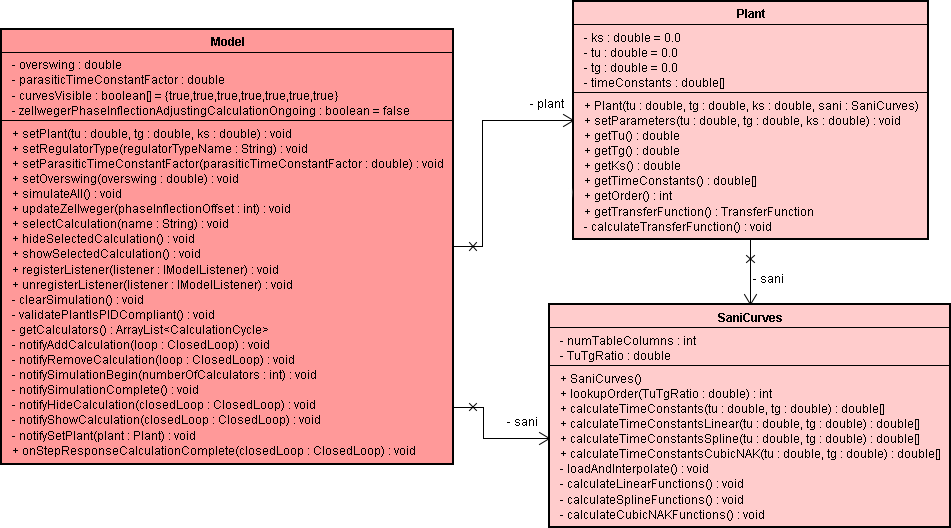
\includegraphics[width=1.00\textwidth]{plant.png}
	\caption{Klassendiagramm der Regelstrecke}
	\label{fig:plant}
\end{figure}


Die Sani-Kurven sind die Grundlage zur Berechnung der \textit{TransferFunction} und die \textit{TransferFunction} ist die Grundlage zur sp�teren Berechnung der Schrittantwort.

Die Sani-Kurven werden nicht vom Programm selbst berechnet, sondern werden zu Programmbeginn aus einer Text-Datei importiert, welche wiederum von Matlab exportiert wurde. Da die Kurven als diskrete Punkte gespeichert sind, werden sie beim Importieren in Java kubisch
interpoliert, um eine h�here Aufl�sung zu erm�glichen. Das Interpolieren erfolgt mittels der \textit{SplineNAK}-Klasse, welche von C in Java �bersetzt wurde. (http://www.pcs.cnu.edu/~bbradie/cpp/interp.C). \\
Da diese Interpolationsmethode mit der in Matlab verwendeten �bereinstimmt, wird ein stabiler Benchmark f�r Tests erm�glicht.
%Die Interpolationsmethode ist die gleiche der in Matlab verwendet wird, was uns ein
%stabiler Benchmark f�rs Testen erm�blicht.

Das \textit{SaniCurves}-Objekt wird nur einmal im \textit{Model} erstellt, um die Festplattenzugriffszeit zu minimieren. Das \textit{Model}-Objekt hat zu jedem Zeitpunkt eine Referenz auf den aktuellen \textit{Plant}.

Jedes Mal, wenn sich mindestens einer der drei Parameter $T_u$, $T_g$ oder $K_r$ im \textit{Plant}-Objekt �ndert, sei es durch eine Instanzierung oder durch Aufrufen der Methode \textit{Plant::setParameters()}, werden mittels \textit{SaniCurves} die Zeitkonstanten
der Strecke und die �bertragungsfunktion neu berechnet.

%Problem/Fragestellung:
%- Wie werden die Sani-Kurven geladen, behandelt und gekapselt?
%L�sung: Die Kurven werden aus einer .txt-Datei ins Java-Programm geladen. Die Kurven werden mittels
%einer Interpolationsmethode aus der Apache-Library interpoliert.
%Erg�nzung: Auch beschreiben wie die Regelstrecke gespeichert wird (Objekt) falls das so ist.


\subsubsection{Regler}

Der Regler, im Programm vom Englischen als \textit{Controller} benannt, beschreibt den Regler der Strecke anhand einer \textit{TransferFunction} (�bertragungsfunktion).

Nicht alle Regler haben gemeinsame Parameter. Bei den verschiedenen Reglertypen sind die Parameter anders benannt oder gar nicht vorhanden. Beispielsweise hat der PI-Regler die Parameter $T_u$ und $T_g$, aber es fehlen die PID-Parameter $T_v$ und $T_p$. Ausserdem wird abh�ngig vom Reglertyp die �bertragungsfunktion anders berechnet. Es gibt aber auch Gemeinsamkeiten, wie der Name oder die Farbe des Reglers und die Tatsache, dass die Parameter in einer Tabelle eingef�gt werden m�ssen. F�r den Rest des Programms ist ausserdem nicht ersichtlich, um was f�r einen Reglertyp es sich handelt. F�r die Schrittantwort wird lediglich die �bertragungsfunktion verwendet.

Aus diesen Gr�nden arbeiten wir hier mit Vererbung. Die Klassen \textit{ControllerI}, \textit{ControllerPI} und \textit{ControllerPID} implementieren jeweils die Details der entsprechenden Reglertypen. Die Superklasse \textit{AbstractController} stellt eine gemeinsame Schnittstelle zur Verf�gung.

\begin{figure}[h]
	\centering
		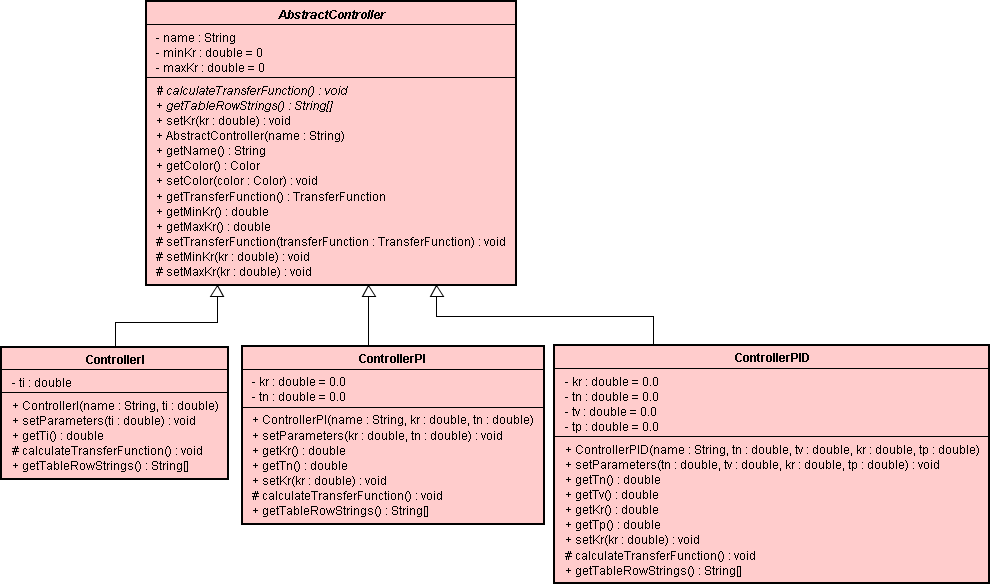
\includegraphics[width=1.00\textwidth]{controller.png}
	\caption{Klassendiagramm des Reglers}
	\label{fig:controller}
\end{figure}


Immer, wenn sich die Reglerparameter �ndern, also dann wenn der Regler instanziert wird, wird seine �bertragungsfunktion berechnet. Diese ist mittels der Methode \textit{AbstractController::getTransferFunction()} abrufbar.

Jeder Regler definiert eine Farbe und einen Namen f�r den Plot. Auf diese Informationen kann mittels der Methoden \textit{AbstractController::getName()} und \textit{AbstractController::getColor()} zugegriffen werden.

Die erbenden Klassen implementieren die Methode \textit{getTableRowStrings()}, welche erlaubt, die Reglerparameter �ber die Superklasse in die Tabelle zu einzuf�gen ohne zu wissen, um was f�r einen Reglertypen es sich handelt.

Wurde der Regler mittels einer Zellwegermethode berechnet, kann ein Fenster f�r den Minimal- und den Maximalwert des Parameters $K_r$ �ber die Methoden \textit{Abstract\-Controller::get\-Min\-Kr()} und \textit{AbstractController::getMaxKr()} geholt werden. Dieses Fenster wird f�r das iterative Approximieren des �berschwingens verwendet. Alle anderen Berechnungsmethoden, also die Faustformeln, berechnen diese Fenster nicht.



%Problem/Fragestellung:
%- Wie werden die Reglertypen (PI und PID) softwaretechnisch entkoppelt?
%- Was gibt es f�r Berechnungen?
%- Wie werden die Reglerberechnungsarten (Zellweger und Faustformeln) softwaretechnisch entkoppelt?
%L�sung: Um die verschiedenen Reglertypen zu entkoppeln wird eine abstrakte Klasse erstellt. Von dieser erben wiederum je eine abstrakte Klasse f�r die Faustformeln und eine abstrakte Klasse f�r die
%Zellweger-Methode.



\subsubsection{Reglerberechung}

Die Reglerberechnung ist hierarchisch und technisch das komplizierteste Teilst�ck des Programms. Es gibt insgesamt 15 verschiedene Klassen, die auf 15 verschiedene Arten einen passenden Regler f�r eine Strecke berechnen k�nnen. Alle erben von der Klasse \textit{AbstractControllerCalculator}.

\begin{figure}[h]
	\centering
		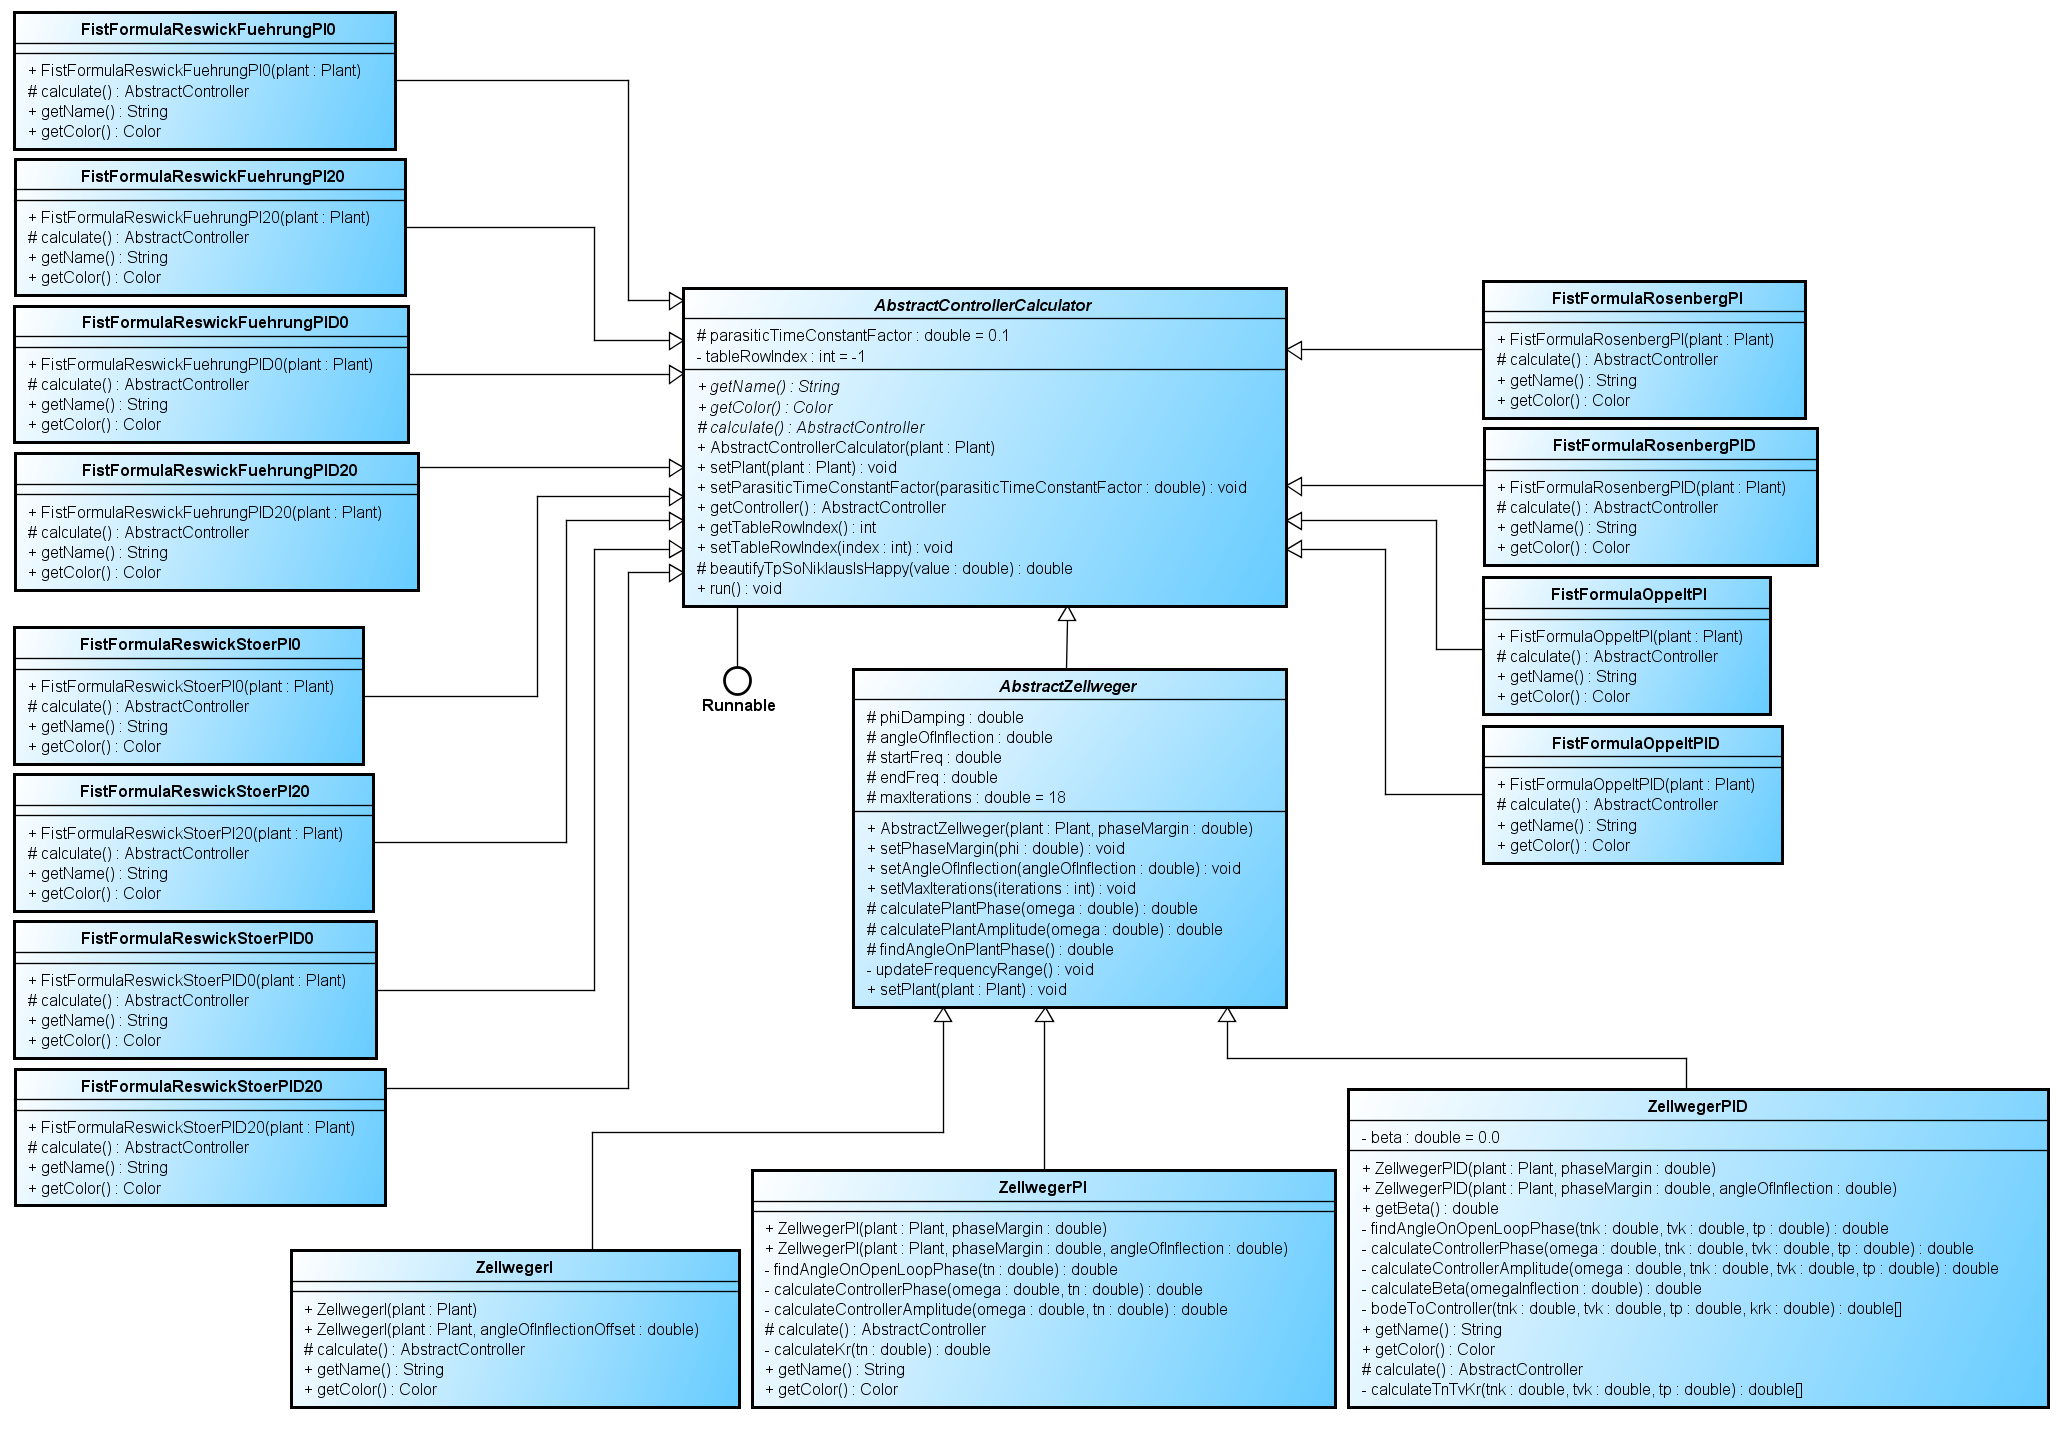
\includegraphics[width=1.00\textwidth]{controller-calculator.png}
	\caption{Klassendiagramm zur Reglerberechnung}
	\label{fig:controller-calculator}
\end{figure}


Grundlegend kann ein neues \textit{ControllerCalculator}-Objekt mit einem \textit{Plant}-Objekt (die Strecke) instanziert werden, es kann
\textit{AbstractControllerCalculator::run()} aufgerufen werden, und es kann mittels der Methode \textit{AbstractControllerCalculator::getController()} der resultierende Regler als \textit{AbstractController} geholt werden.

Wie der Regler berechnet wird und welchem Typ der Regler angeh�rt, ist dabei durch die Vererbung abstrahiert.



\subsubsection{Regelkreis}

Mit der Klasse \textit{ClosedLoop} kann mit einem \textit{Plant}-Objekt und einem \textit{AbstractController}-Objekt ein geschlossener Regelkreis erstellt werden. Auch der \textit{ClosedLoop} hat eine �bertragungsfunktion (ein \textit{TransferFunction}-Objekt), welche aus den �bertragungsfunktionen der Strecke und des Reglers berechnet wird.

\begin{figure}[h]
	\centering
		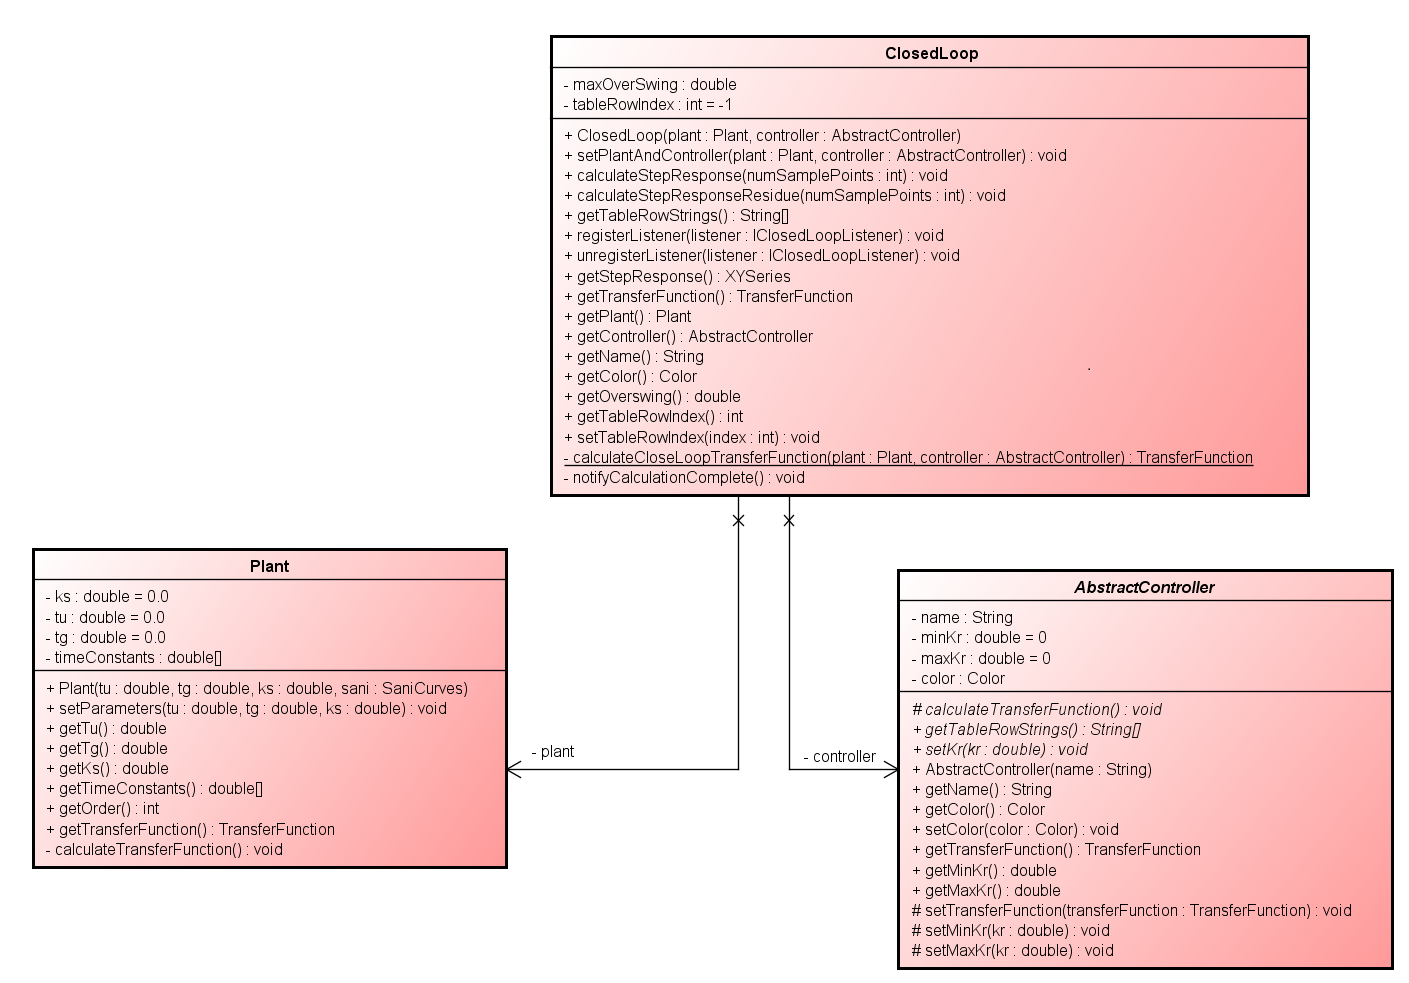
\includegraphics[width=1.00\textwidth]{closed-loop.png}
	\caption{Klassendiagramm zum Regelkreis}
	\label{fig:closed-loop}
\end{figure}


Immer wenn sich das \textit{Plant}-Objekt oder das \textit{AbstractController}-Objekt �ndern, sei es durch eine Instanzierung oder durch Aufrufen der Methode \em{ClosedLoop::setPlantAndController()}, wird aus den beiden �bertragungsfunktionen des \textit{Plant}-Objektes und des \textit{AbstractController}-Objektes die �bertragungsfunktion des geschlossenen Regelkreises berechnet.

Durch Aufrufen der Methode \textit{ClosedLoop::calculateStepResponse()} wird die Sprungantwort mittels der Residuenmethode berechnet. Die resultierende Schrittantwort kann mit der Methode \textit{ClosedLoop::getStepResponse()} als \textit{XYSeries} f�r JFreeChart geholt werden. Die Residuenmethode wurde gew�hlt, da sie robuster und schneller ist als die Variante mit IFFT. Ein Vergleich dazu ist im Abschnitt Validierung unter \ref{residuenvsifft} aufgef�hrt.

Weiter wird bei der Berechnung der Sprungantwort das maximale �berschwingen gemessen. Dieser Wert kann mit der Methode \textit{ClosedLoop::getOverswing()} geholt werden.



\subsubsection{Resultate}

Die Resultate der Berechnungen sind die Reglerparameter $T_n$, $T_v$ und $K_r$, die parasit�re Zeitkonstante $T_p$, das �berschwingen, der Name der verwendeten Methode und die Schrittantwort. 

Die Schrittantworten werden mit JFreeChart geplottet und die restlichen Parameter k�nnen mit der Methode \textit{AbstractController::getTableRowStrings()} als String-Array geholt werden und werden im GUI in eine Tabelle eingef�gt.

%Problem/Fragestellung:
%- Was wird berechnet?
%- Wie werden die berechneten Resultate gespeichert?
%- Wie werden die Resultate im User-Interface dargestellt?
%L�sung: Die berechneten Regler-Parameter werden in einer Tabelle im User-Interface dargestellt. Die
%Sprungantworten werden in einem Plot dargestellt.

%\graphicspath{{./PrettyPictures/}}


\subsection{View}
Die Klasse \textit{View} und ihre Unterklassen sind zust�ndig f�r die Darstellung der Benutzeroberfl�che. Am oberen Fensterrand befindet sich die \textit{MenuBar}, welche sich �ber die gesamte Breite erstreckt. Sie enth�lt Einstellungsm�glichkeiten und weiterf�hrende Informationen. Auf der linken Seite befinden sich zwei Panels f�r die Ein- und Ausgabe. Im \textit{InputPanel} k�nnen die Eingabeparameter eingetragen, der gew�nschte Regler und das �berschwingen gew�hlt und die Simulation mit einem Button gestartet werden. Das \textit{OutputPanel} stellt alle berechneten Graphen mit der Angabe ihrer Kennwerte in einer Tabelle dar und besitzt einen Trimmer f�r das manuelle justieren des Phasenwinkels. Auf der rechten Seite des Fensters werden die Graphen mit der Klasse \textit{GraphPanel} angezeigt. Unter diesem Plot befindet sich das \textit{GraphDisplayPanel} und das \textit{GraphSettingPanel}, welche beide f�r f�r die Auswahl der darzustellenden Kurven verantwortlich sind. Im folgenden Abschnitt wird die Darstellung des GUIs (Graphical User Interface) genauer erl�utert.

\subsubsection{Anforderungen an die Benutzeroberfl�che}
%Problem/Fragestellung:
%- Was sind die Anforderungen des Auftraggebers und wie wurde das GUI gestaltet?
%- Welche Zusatzfunktionen wurden implementiert?
%- Was wurde beachtet, damit das Tool intuitiv bedient werden kann?
%L�sung: Die Anforderungen wurden gemeinsam im Team und im Gespr�ch mit dem Auftraggeber besprochen. Die einzelnen Entscheidungen werden jeweils begr�ndet.
Die Benutzeroberfl�che wurde so umgesetzt, dass der Anwender das Tool intuitiv bedienen kann und es einen grafisch ansprechenden Eindruck hinterl�sst. Des Weiteren wird nach Wunsch des Auftraggebers das Programm in einem einzelnen Fenster dargestellt. Dies erm�glicht es dem Anwender, alles zu �berblicken und mit einem einzigen Printscreen das gesamte Programm (Einstellungen, Graph) in einer Dokumentation festzuhalten oder mit anderen Methoden zu vergleichen. Dies f�hrt zu einer einfacheren Handhabung der erstellten Simulationen.

Vom Auftraggeber wurden folgende Punkte f�r die Benutzeroberfl�che gew�nscht:
\begin{itemize}
	\item Es soll lediglich der Graph der Schrittantwort dargestellt werden.
	\item Eine automatische Skalierung �ber einen sinnvollen Bereich f�r den Graphen soll implementiert sein. Falls dies nicht gelingt, sollten die Achsen manuell einstellbar sein.
	\item Das im Graphen ausgemessene �berschwingen soll in einer Tabelle dargestellt werden.
	\item Die Fenstergr�sse soll ver�nderbar sein, zus�tzlich sollte eine Miniversion enthalten sein.
	\item Alle Informationen sollten in einem Fenster angezeigt werden, sodass mit einem Blick alles erkannt werden kann.
\end{itemize}

%\textbf{Zusatzfunktionen}
%Die folgenden Zusatzfunktionen wurden in das Tool integriert:
%\begin{itemize}
	%\item Approximation des �berschwingens an einen frei w�hlbaren Wert.
	%\item Ver�nderung des Phasenwinkels mittels eines Trimm-Sliders.
	%\item Export der gesamten Ansicht als PDF.
	%\item Hilfreiche Links im Menu Hilfe.
%\end{itemize}


%TODO JOSUA:
%- Alles oberhalb korrigierten!
%- Was vom oben geschriebenen ist wie implementiert?
%- Wie wurde das GUI gestaltet? -> Begr�nden der Entscheide.
%- Wie konnte die Bedienung intuitiv gestaltet werden?


\subsubsection{Erstellung der Benutzeroberfl�che}
%Problem/Fragestellung:
%- Wie wurden die Anforderungen und die Zusatzfunktionen des Auftraggebers umgesetzt?
%- Was waren die �berlegungen bez�glich der Gr�sse des Tools, der Aufteilung der Panels und der
%Platzierung der Komponenten?
%L�sung: Die Benutzeroberfl�che wurde im Team besprochen und dem Auftraggeber pr�sentiert. Die
%technische Umsetzbarkeit der einzelnen W�nsche wurde �berpr�ft.
F�r die Erstellung der Benutzeroberfl�che wurden haupts�chlich die Swing-Klassen der Java Foundation Classes (JFC) verwendet. Sie enthalten die notwendigen Komponenten wie Textfelder, Buttons usw., mit denen grafische Oberfl�chen erstellt werden k�nnen. Erkennbar sind sie auch durch das "`J"', welches dem Namen vorangestellt ist (beispielsweise JButton). Auf die ausf�hrliche Beschreibung dieser Standardkomponenten wird bewusst verzichtet und es werden nur die zus�tzlichen Komponenten erl�utert, welche verwendet wurden.\\
F�r die Platzierung der Komponenten gibt es in Java verschiedene Layoutmanager, um die Komponenten anzuordnen. Um einen kurzen �berblick �ber diese Manager zu geben, werden die verwendeten in der folgenden Aufz�hlung kurz beschrieben:

\begin{enumerate}
	\item \textit{GridBagLayout}: Er ist der m�chtigste LayoutMangager aus dem Java AWT-Package und erm�glicht es, die Komponenten in ein anpassbares Raster (Grid) zu setzen. Die einzelnen Spalten k�nnen dabei unterschiedlich breit und die einzelnen Zeilen unterschiedlich hoch sein. Die Komponenten werden in eine Zelle gesetzt und k�nnen von dort in X- und Y-Richtung weitere Zellen �berlappen. Weiter gibt es viele zus�tzliche Anpassungsm�glichkeiten.
	\item \textit{GridLayout}: Setzt die Komponenten in ein gleichm�ssiges Raster (Grid), bei dem alle Zellen die selbe Gr�sse haben.
	\item \textit{BorderLayout}: Besitzt f�nf Bereiche (Norden, S�den, Osten, Westen, Zentrum), in welche Komponenten platziert werden k�nnen.
	\item \textit{WrapLayout}: Alle Komponenten werden nacheinander von links nach rechts eingef�llt. Beim Ver�ndern der Fenstergr�sse gibt es Zeilenumbr�che, falls die Breite des Panels nicht mehr ausreicht. Dieses Layout geh�rt nicht zu den Standard-Typen und wird bei der Erl�uterung des \textit{GraphDisplayPanels} genauer beschrieben.
\end{enumerate}

F�r weitere Informationen zu Layoutmanagern wird auf die Dokumentation von Oracle verwiesen \cite{OracleDoc}.

\textbf{Aufbau der Benutzeroberfl�che}\\
Der Aufbau des GUIs wurde so erstellt, dass die gesamte grafische Benutzeroberfl�che in einem JFrame platziert ist. Dieses Frame enth�lt jeweils eine Instanz der  Klasse \textit{MenuBar} und \textit{View}. Die \textit{View} besteht wiederum aus den vier JPanels \textit{InputOutputPanel}, \textit{GraphPanel}, \textit{GraphDisplayPanel} und \textit{GraphSettingPanel}. Das \textit{InputOutputPanel} fasst das \textit{InputPanel} und das \textit{OutputPanel} zu einem gemeinsamen JPanel zusammen. Auf die Layoutmanager wird bei der Beschreibung der einzelnen Panels genauer eingegangen. \\

In der folgenden Grafik wurde der gesamte Zusammenhang dargestellt: 

\begin{figure}[h]
	\centering
		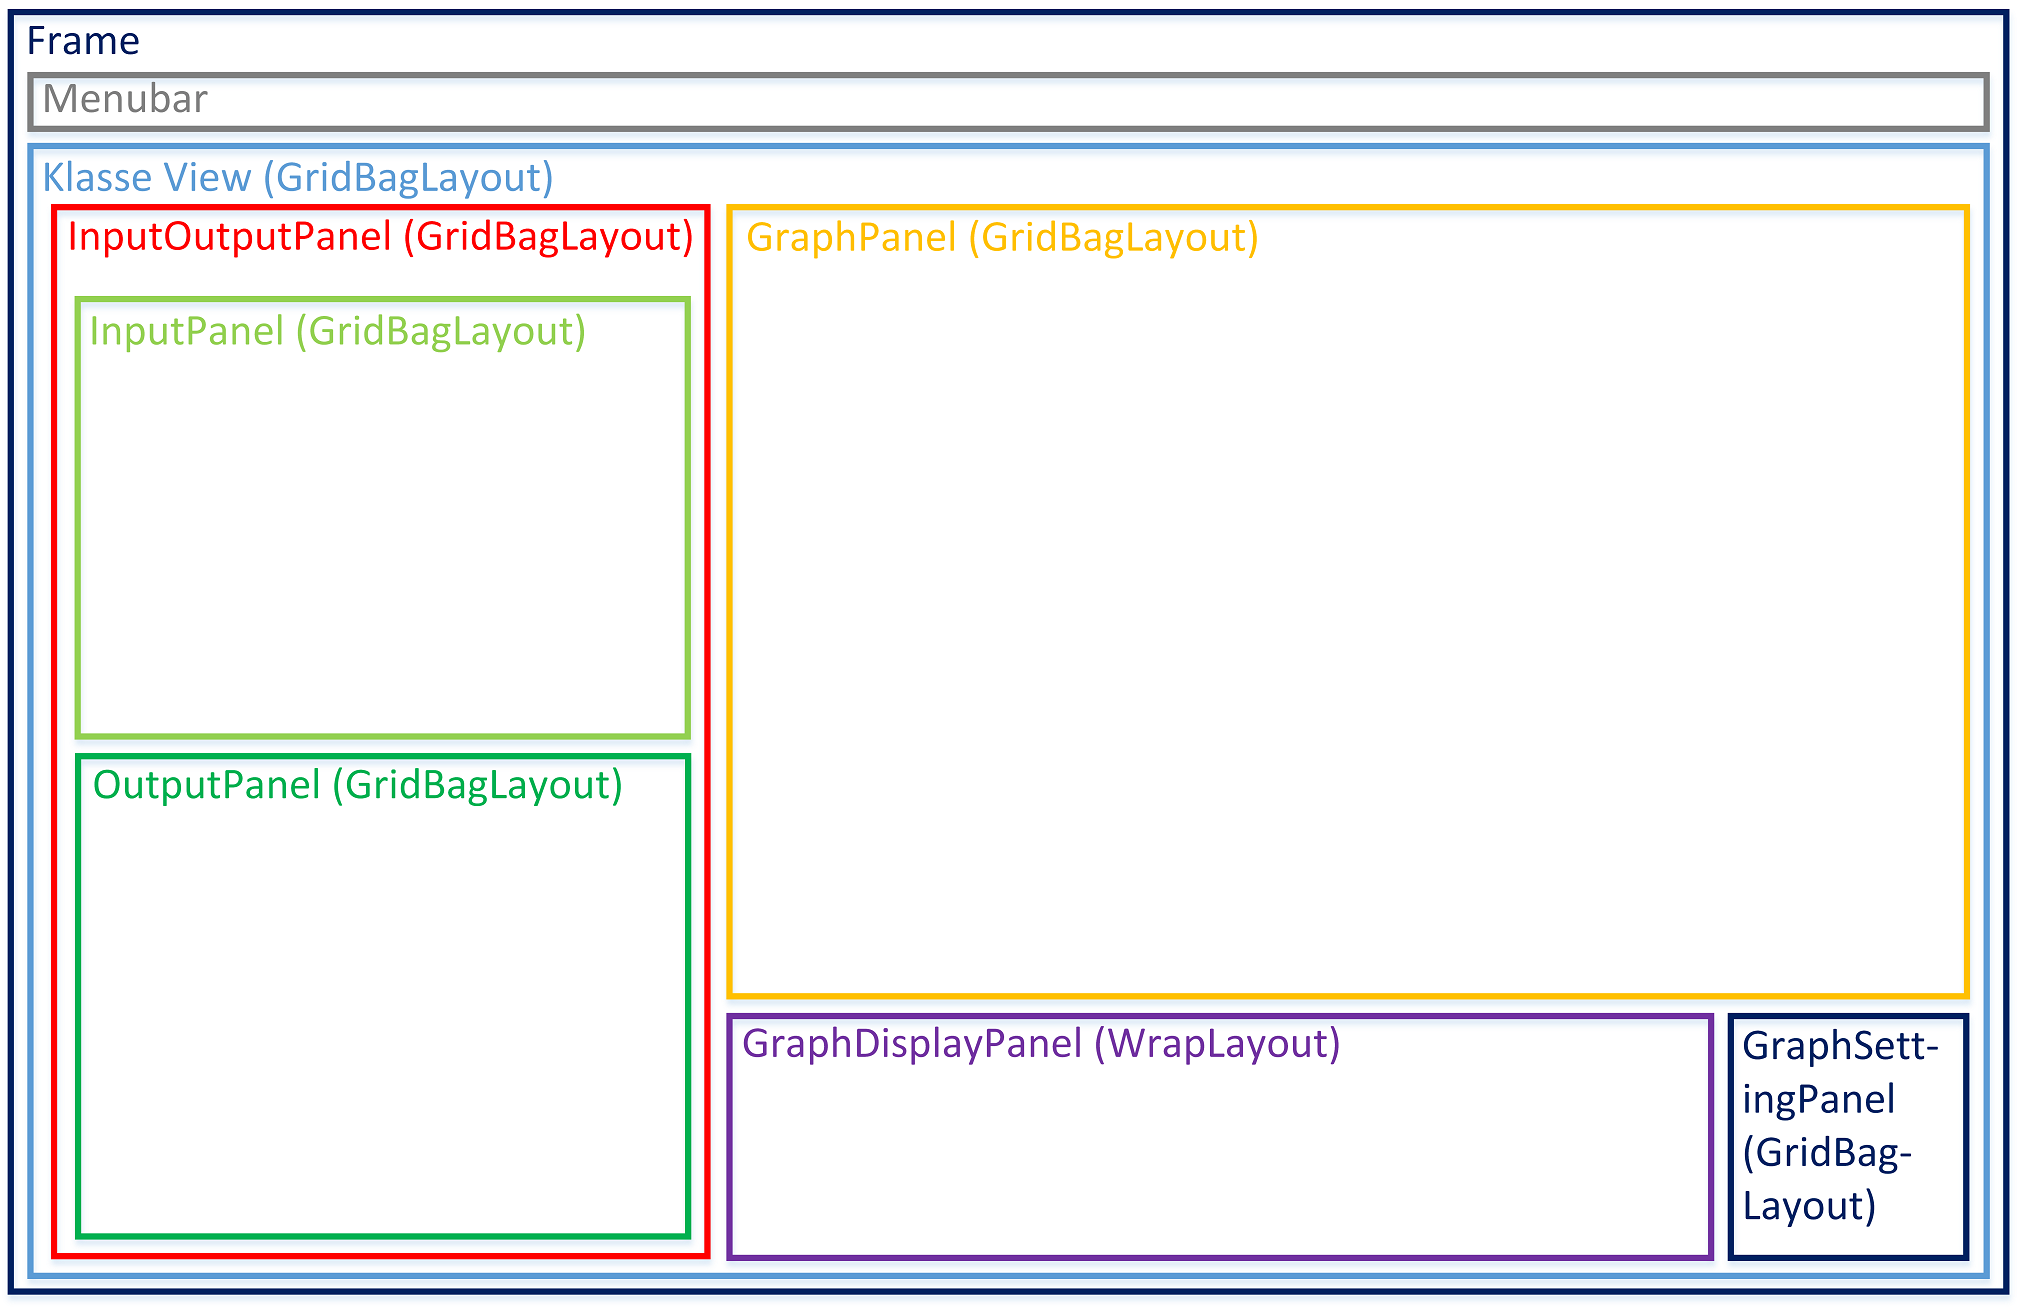
\includegraphics[width=12cm]{Panels.png}
	\caption{Aufbau des GUIs}
	\label{fig:Aufbau der Benutzerfl�che}
\end{figure}

\subsubsection{Aufgabe der einzelnen Panels}
Die Benutzeroberfl�che beinhaltet, wie vorhin beschrieben, mehrere Panels. Das \textit{Input\-Panel} dient zur Eingabe der Kenngr�ssen der Regelstrecke und das \textit{OutputPanel} zur Anzeige der berechneten Reglerparameter und zur nachtr�glichen Manipulation des Phasenwinkels. Das \textit{GraphPanel} visualisiert die Schrittantwort, das \textit{GraphDisplayPanel} erm�glicht die Auswahl der anzuzeigenden Kurven und das \textit{GraphSettingPanel} besitzt drei Buttons f�r die Einstellungen zum Graphen. Ein Grossteil der verwendeten Komponenten stammt aus der Swing Klasse von Java, alle zus�tzlichen werden speziell erl�utert. Folgend werden die Panels genauer beschrieben:\\

\begin{figure}[h]
	\centering
		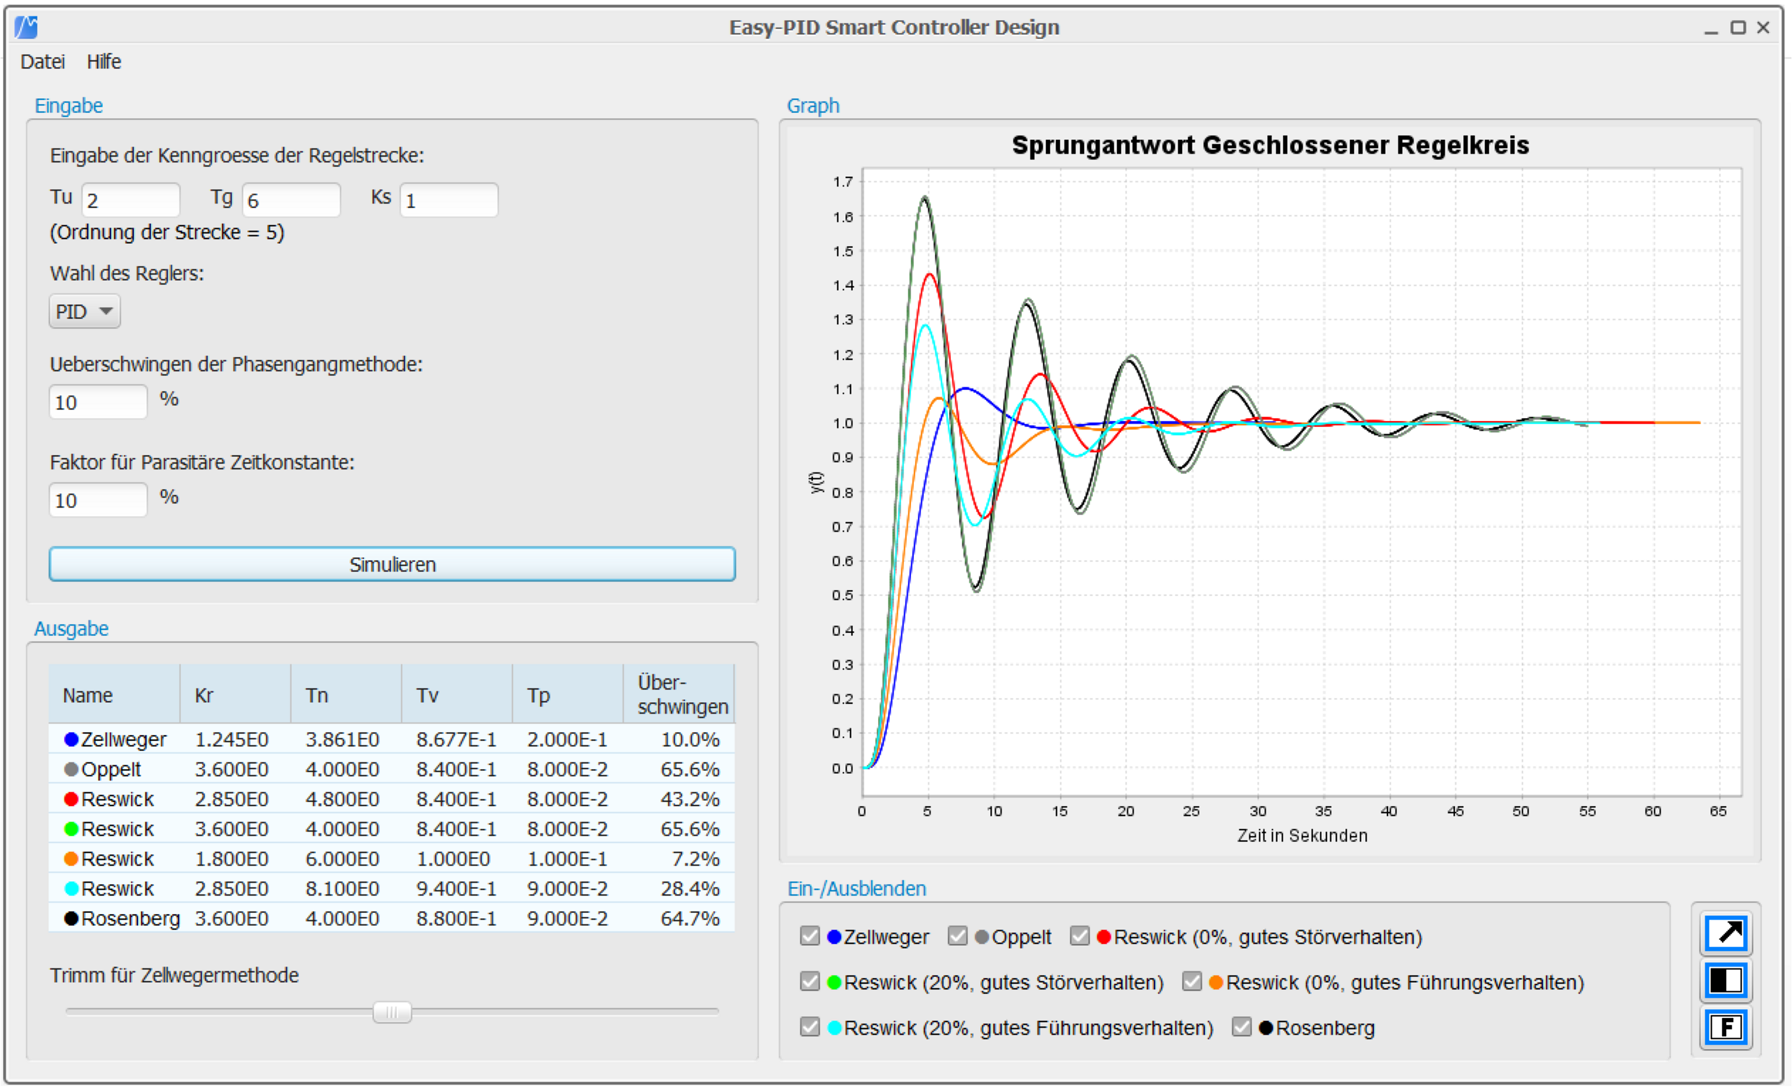
\includegraphics[width=16cm]{GUI.png}
	\caption{�bersicht �ber das GUI}
	\label{fig:Aufgabe der einzelnen Panels}
\end{figure}

\textbf{InputOutputPanel:} Die Aufgabe dieses im GridBagLayout erstellten Panels besteht einzig darin, das \textit{InputPanel} und das \textit{OutputPanel} in einem gemeinsamen Panel zu vereinen. Dieses Panel wurde erstellt, um die Handhabung im GridBagLayout der Klasse \textit{View} zu verbessern. \\

\textbf{InputPanel:} Dieses Panel wurde im GridBagLayout erstellt und besitzt einen Rahmen mit dem Titel "`Eingabe"'. Es enth�lt zuoberst die drei Eingabefelder f�r die Parameter \textit{Tu} (1), \textit{Tg} (2) und \textit{Ks} (3) der Regelstrecke. Anschliessend folgt eine leere Zeile, die zu Beginn keinen Inhalt hat. Sie zeigt nach einer Simulation den Grad der Berechnung an und bei fehlerhaften Eingaben rote Hinweise f�r den Anwender. Als n�chstes folgt das Dropdown-Men� f�r die Auswahl des Reglers (4) (\textit{I}, \textit{PI} oder \textit{PID}). In den n�chsten beiden Textfeldern (4 und 5) kann das �berschwingen und die parasit�re Zeitkonstante eingetragen werden. Diese beiden Eingaben  sind abh�ngig von der Auswahl des Reglers und deshalb nicht f�r alle Regler aktiviert. Wenn die Felder deaktiviert sind, werden sie ausgegraut und es k�nnen keine Werte eingetragen werden. Beim I-Regler werden beide und beim PI-Regler nur das Feld f�r die parasit�re Zeitkonstante deaktiviert. Beim PID-Regler sind beide aktiviert. Am Ende dieses Panels befindet sich �ber die gesamte Breite die Schaltfl�che zum Starten der Simulation (7).

Alle Beschriftungen sind JLabels, alle Textfelder sind JFormatedDoubleTextfields, die Schaltfl�che ist ein JButton und f�r die Wahl des Reglers wurde eine JComboBox verwendet. Weiter verf�gen alle Textfelder �ber ToolTips (Zusatzinformationen bei Objekten), welche dem Nutzer zus�tzliche Informationen bieten. 

\begin{figure}[h]
	\centering
		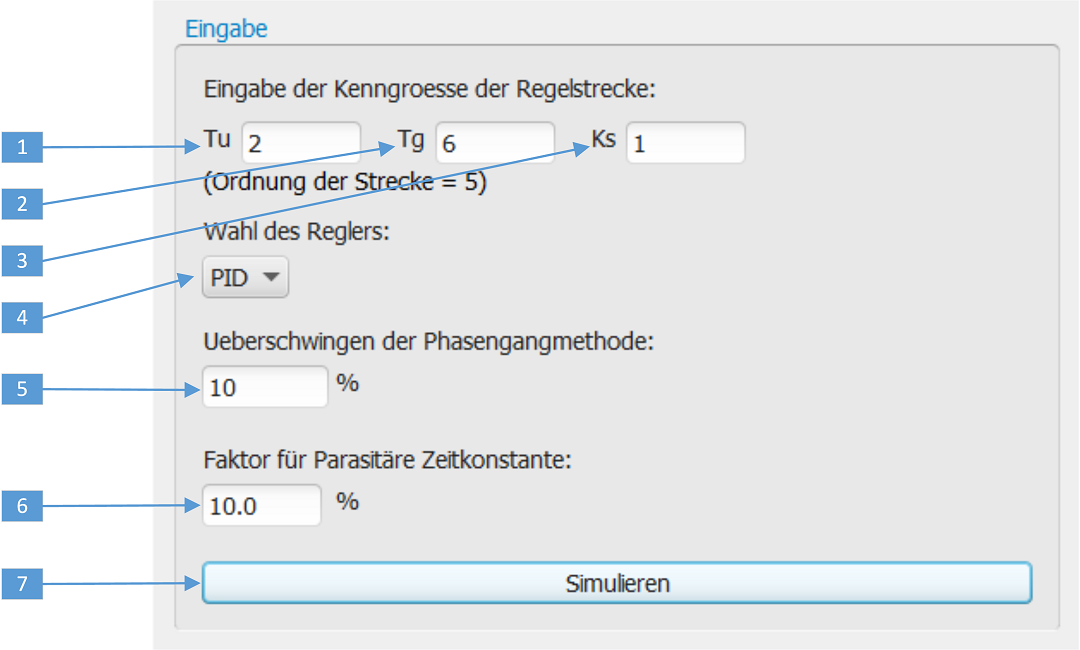
\includegraphics[width=12cm]{InputPanel.png}
	\caption{InputPanel}
	\label{fig:InputPanel}
\end{figure}

\textbf{OutputPanel:} Dieses Panel wurde im GridBagLayout erstellt und besitzt einen Rahmen mit dem Titel "`Ausgabe"'. In einer �bersichtlichen Tabelle werden alle Kennwerte jeder simulierten Kurve aufgelistet. Diese Tabelle besteht aus den sechs Spalten mit den folgenden Inhalten:
\begin{enumerate}
	\item \textit{Name}: Als erstes steht ein grosser farbiger Kreis in der Farbe der dazugeh�renden Kurve. Dadurch kann der Anwender den Zusammenhang zwischen Tabelle, Graph und Auswahl der Kurven leicht erkennen. Nach dem Kreis folgt im selben Feld der Name des Reglers. 
	\item \textit{Kr}: Enth�lt den berechneten Wert f�r die Reglerverst�rkung
	\item \textit{Tn}: Enth�lt den berechneten Tn-Reglerparameter 
	\item \textit{Tv}: Enth�lt den berechneten Tv-Reglerparameter
	\item \textit{Tp}: Enth�lt den berechneten Tp-Reglerparameter
	\item \textit{�berschwingen}: Enth�lt das gemessene �berschwingen in Prozent
\end{enumerate}

F�r die nachtr�gliche Optimierung folgt unter der Tabelle ein Slider (\textit{Trimm f�r Zellwegermethode}), mit dem der Phasenwinkel manuell ver�ndert werden kann (7). 
Die Tabelle des \textit{OutputPanels} ist eine JTable mit einem TableHeader und der Slider ein JSlider. 
\\

\begin{figure}[h]
	\centering
		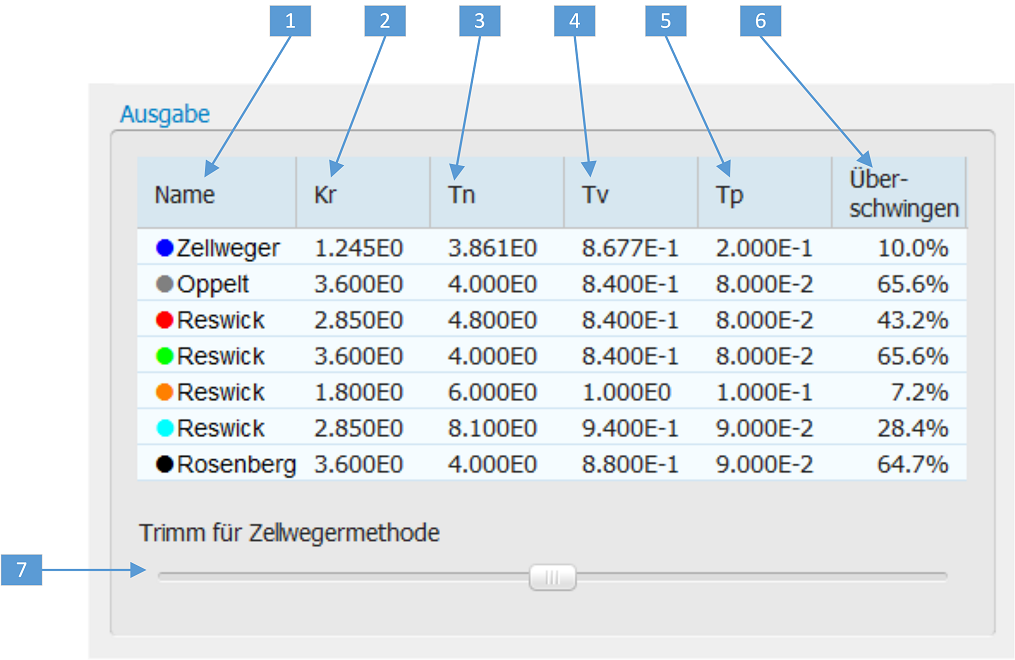
\includegraphics[width=12cm]{OutputPanel.png}
	\caption{OutputPanel}
	\label{fig:OutputPanel}
\end{figure}

\textbf{GraphPanel:} Das \textit{GraphPanel} stellt die Schrittantworten der im \textit{GraphDisplayPanel} ausgew�hlten Regler-Typen dar. Die Achsen werden dabei automatisch skaliert und falls im \textit{GraphDisplayPanel} Anpassungen vorgenommen wurden, werden die einzelnen Kurven ein- oder ausgeblendet. F�r das Anzeigen des Graphen wird ein XYPlot der Klasse \textit{JFreeChart} verwendet, der im BorderLayout platziert wurde. \\

\begin{figure}[h]
	\centering
		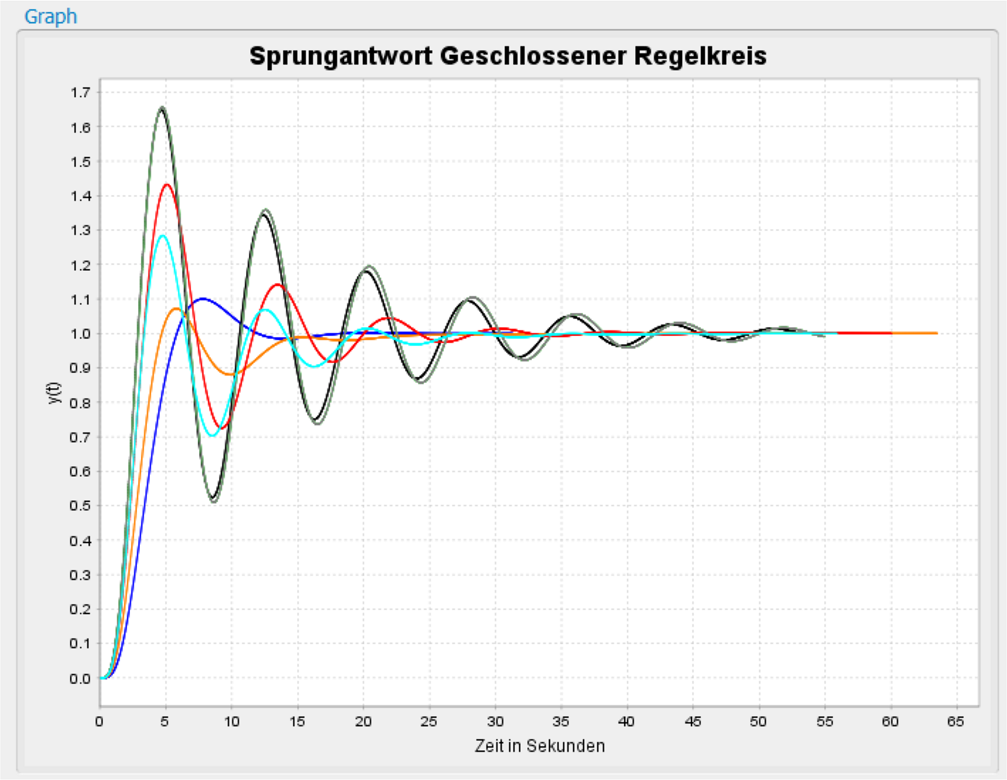
\includegraphics[width=12cm]{GraphPanel.png}
	\caption{GraphPanel}
	\label{fig:GraphPanel}
\end{figure}

\textbf{GraphDisplayPanel und GraphSettingPanel:} Im \textit{GraphDisplayPanel} k�nnen mit Hilfe der Checkboxen die Regler ausgew�hlt werden, welche im \textit{GraphPanel} angezeigt werden sollen (1). Rechts daneben wurde das \textit{GraphSettingPanel} platziert. Dieses zus�tzliche Panel verf�gt �ber drei Buttons mit den folgenden Funktionen:
\begin{itemize}
	\item (2) Zur Original-Ansicht wechseln (Zoom auf 100\%).
	\item (3) Alle Kurven ein-/ausblenden.
	\item (4) Alle Faustformeln ein-/ausblenden.
\end{itemize}

Alle Checkboxen sind JCheckBoxen der Swing-Klassen und die drei Button sind JButtons mit selbst erstellten Icons.

Beim \textit{GraphDisplayPanel} wurde der \textit{WrapLayoutManager} verwendet. Dies ist kein Standard Layoutmanager und wurde auf einem Web-Blog gefunden \cite{WrapLayout}. Dieser Manager ist von der Funktion her vergleichbar mit dem FlowLayout und f�llt alle Komponenten von links nach rechts in ein JPanel. Speziell an ihm ist jedoch, dass er beim Ver�ndern der Fenstergr�sse den Umbruch der Zeilen richtig handhabt, auch wenn das Panel in einem GridBagLayout platziert ist. 

\begin{figure}[h]
	\centering
		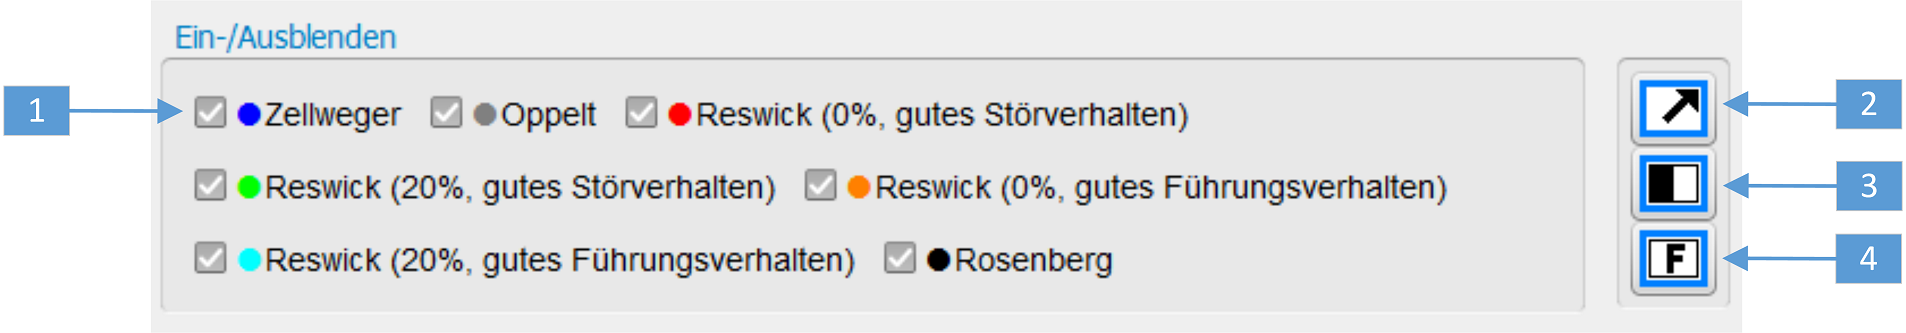
\includegraphics[width=12cm]{GraphDisplayPanel.png}
	\caption{GraphDisplayPanel}
	\label{fig:GraphDisplayPanel und GraphSettingPanel}
\end{figure}

Ausserdem befindet sich am oberen Rand des Fensters die \textit{MenuBar} mit den beiden Schaltfl�chen \textit{Datei} und \textit{Hilfe}. Sie wurde direkt ins Frame gesetzt und wurde nicht in der Klasse \textit{View} hinzugef�gt.\\

Das Men� \textit{Datei} besteht aus den folgenden Men�eintr�gen:
\begin{itemize}
	\item \textit{Zur Mini-Version wechseln}: Wechselt von der Gesamtansicht zur Mini-Version. Elemente wie das \textit{GraphPanel}, das \textit{GraphDisplayPanel} und der Trimmer werden dabei ausgeblendet. Der Name dieses Men�eintrages �ndert sich von Mini-Version zu Normal-Version.
	\item \textit{Export als PDF}: �ffnet ein Fenster, mit dem der Pfad und der Dokumentname ausgew�hlt werden kann. Nach der Best�tigung mit dem Button "`Speichern"' wird ein PDF generiert, welches die gesamte Ansicht des Tools exportiert.
	\item \textit{Schliessen}: Beendet die gesamte Applikation.
\end{itemize}

Das Men� \textit{Hilfe} besteht aus den folgenden Men�eintr�gen:
\begin{itemize}
	\item \textit{Info}: Es �ffnet sich ein Fenster mit Informationen zum Projekt und den Autoren.
	\item \textit{Hilfreiche Links}: Mit ihnen k�nnen Links und PDF-Dokumente ge�ffnet werden, welche weiterf�hrende Information zur Reglerdimensionierung und der Zellweger-Methode bieten.
\end{itemize}

Das gesamte Men� wurde mit Komponenten der Swing-Klassen erstellt.

%TODO JOSUA:
%- Lesen und ev. korrigieren.
\subsubsection{Die Klasse View im Klassendiagramm}
Im folgenden Ausschnitt aus dem Klassendiagramm ist der Zusammenhang der Klasse View zu den Panels und den ganzen Swing-Komponenten dargestellt. F�r das gesamte Klassendiagramm wird auf den Anhang verwiesen. \textbf{(QUELLE ZU KLASSENDIAGRAMM)}

\begin{figure}[h]
	\centering
		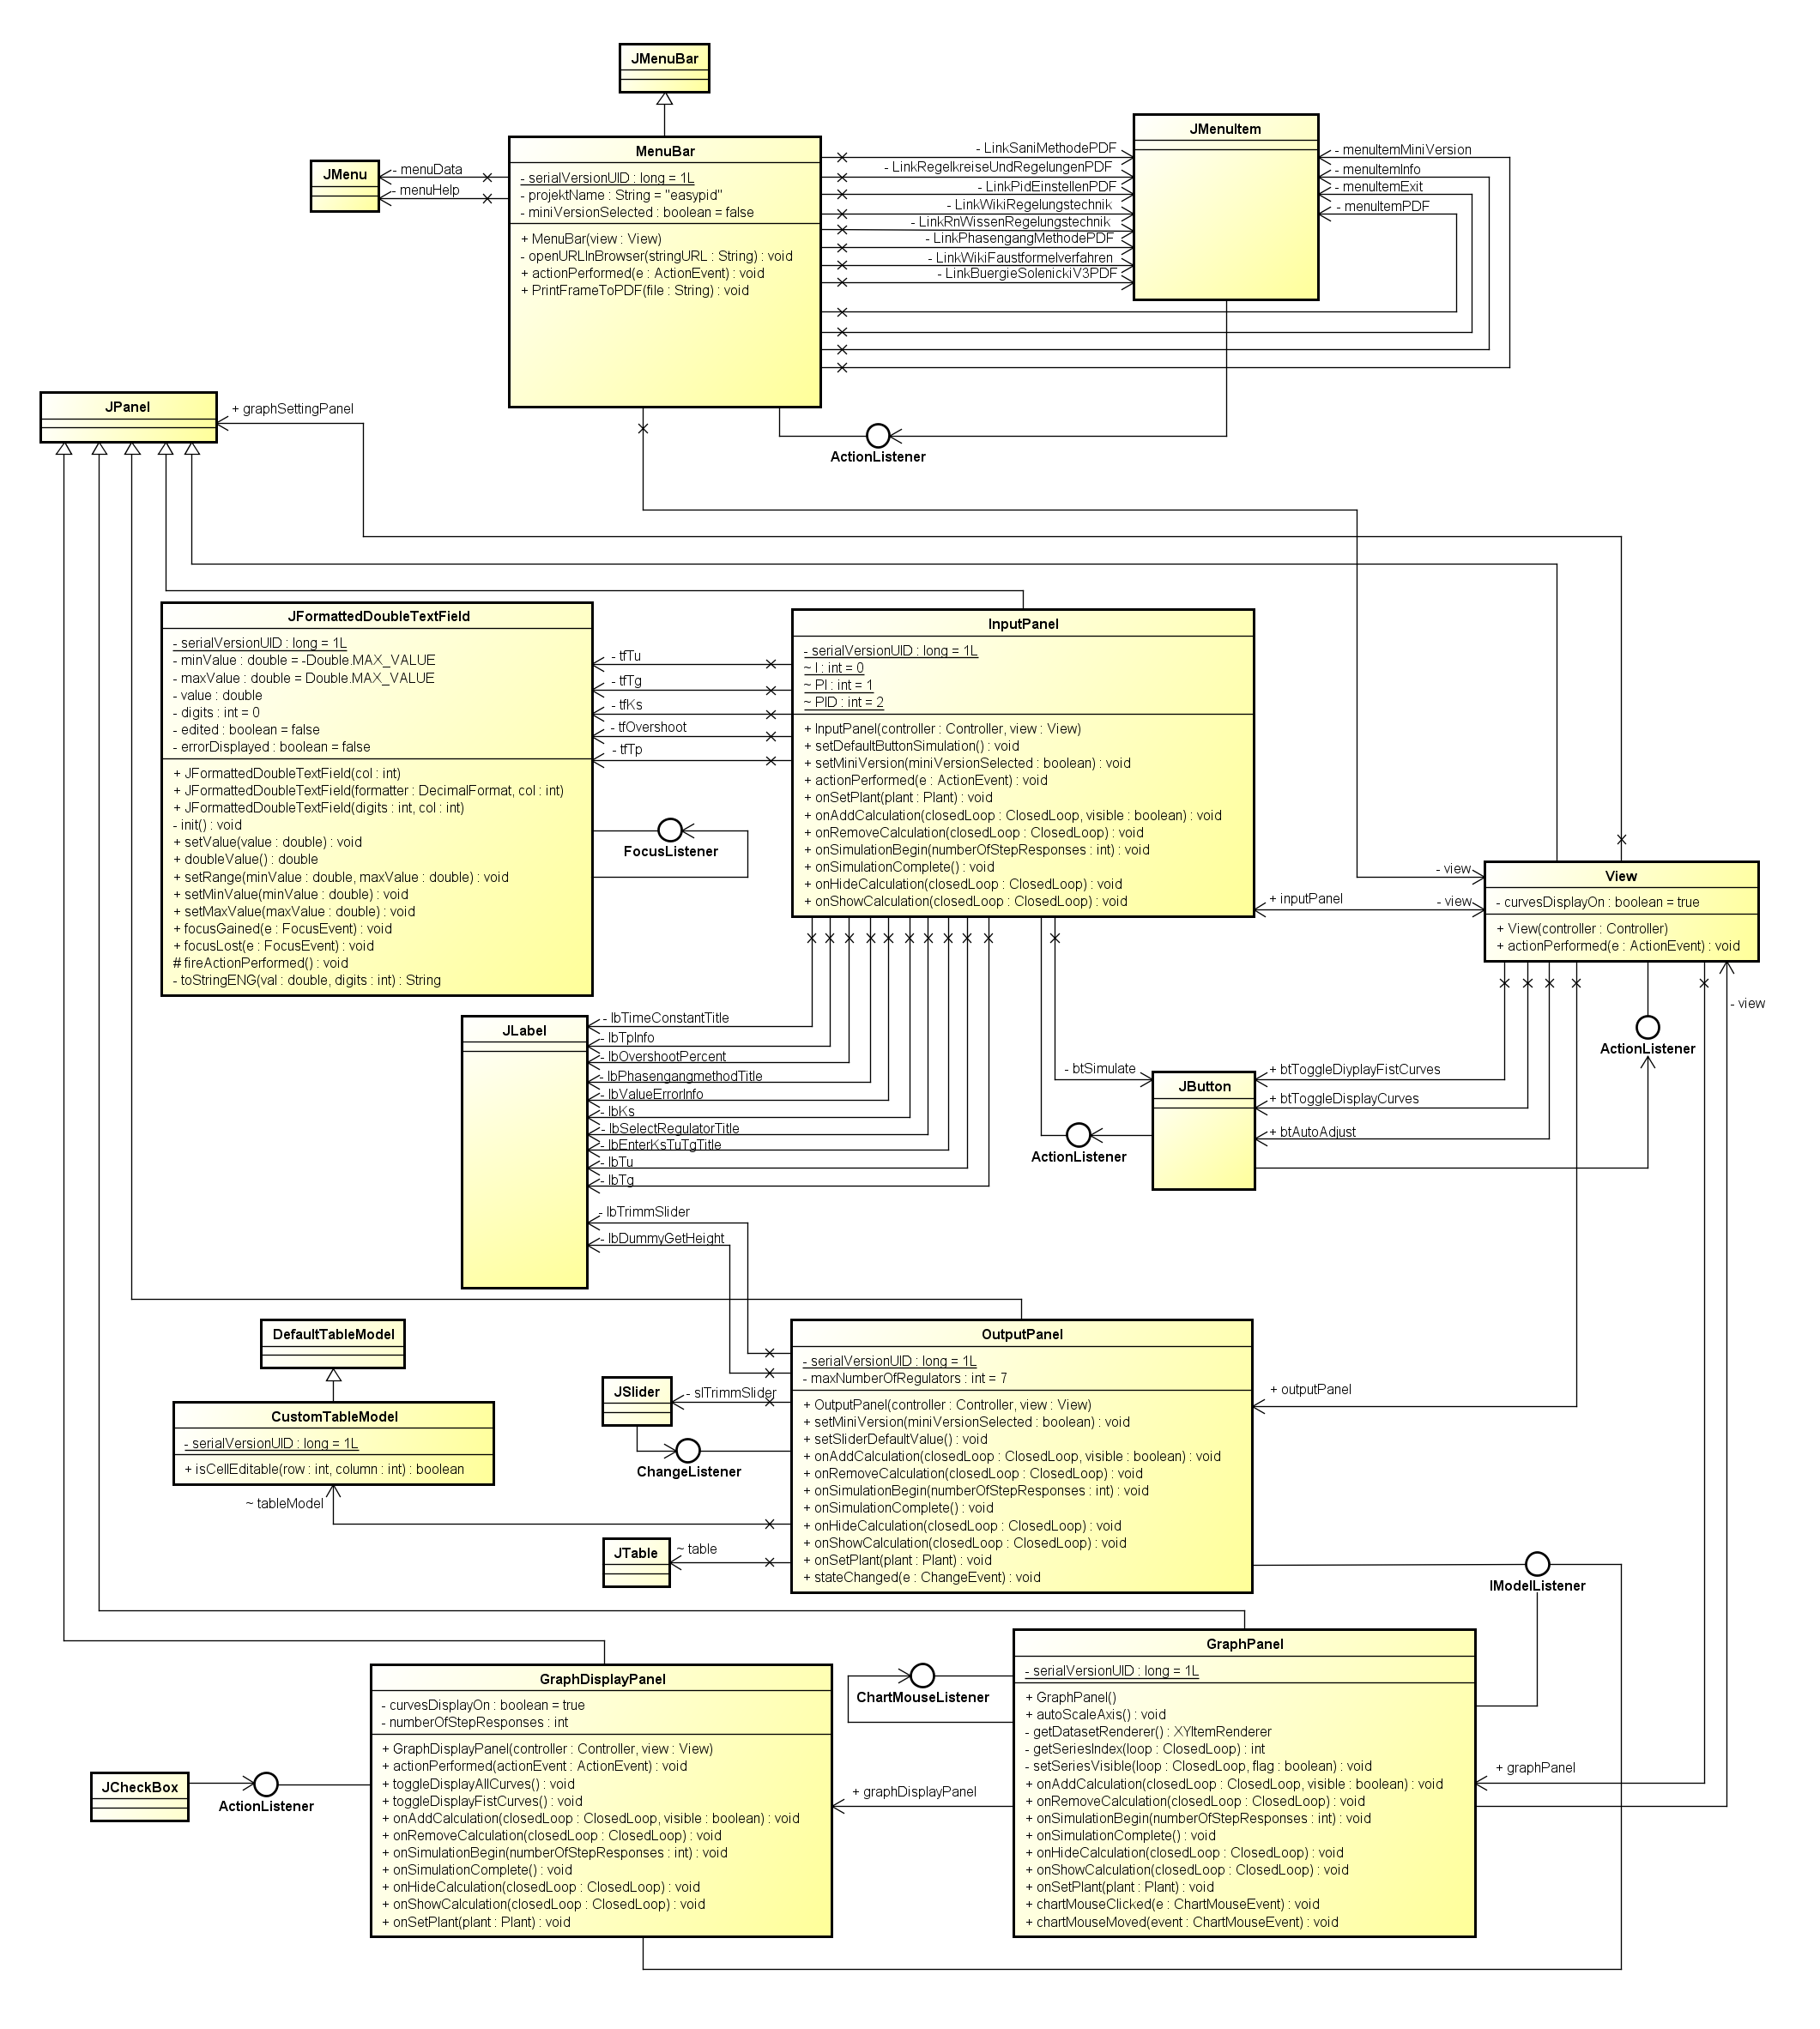
\includegraphics[width=12cm]{Klassendiagramm_View.png}
	\caption{Klasse View und ihre Unterklassen}
	%\label{fig:GraphDisplayPanel und GraphSettingPanel}
\end{figure}

\subsubsection{Funktionalit�t der Benutzeroberfl�che}
%Problem/Fragestellung:
%- Was sind die erlaubten Eingaben in den Textfeldern und wie werden falsche Eingaben gehandhabt?
%- Wie ver�ndern sich die einzelnen Panels wenn die Fenstergr�sse ver�ndert wird?
%- Welche Elemente m�ssen ausgeblendet oder ver�ndert werden, wenn zur Miniversion gewechselt
%wird?
%L�sung: Zu jedem Punkt wird die L�sung pr�sentiert und die L�sungswahl begr�ndet.
\textbf{Eingabewerte}\\
F�r alle Textfelder wurden JDoubleTextFields verwendet. Diese Klasse bekamen wir im Rahmen des Fachinputs durch Herrn Prof. Dr. Richard Gut empfohlen. Sie handhabt die unerlaubten Eingaben der Textfelder. Dabei wurden folgende Einstellungen vorgenommen:
\begin{enumerate}
	\item Die Felder werden nicht gerundet, verf�gen also �ber keinen Formater.
	\item Es k�nnen nur Zahlen, keine Buchstaben und keine anderen Zeichen eingegeben werden (Ausnahme dabei ist das "`e"' f�r Engineering-Eingaben).
	\item Die Fehlermeldung direkt im Textfeld wurde deaktiviert. Fehler werden in diesem Tool auf einer extra Zeile dargestellt.  
\end{enumerate}

\textbf{Fenstermanagement}\\
Wenn das Tool gestartet wird, �ffnet sich das Programm in der Normalansicht (alle Panels werden angezeigt) mit der kleinstm�glichen Fenstergr�sse. Dazu wird das Frame so gepackt, dass alle Komponenten mit ihrer Minimalgr�sse platziert werden. Um das Tool auch bei unterschiedlichen Bildschirmaufl�sungen verwenden zu k�nnen, wurden daf�r keine absoluten Pixelwerte eingesetzt.\\
Wenn die Fenstergr�sse durch den Anwender ver�ndert wird, hat dies einen unterschiedlichen Einfluss auf die einzelnen Panels. Das \textit{OutputPanel} wird nur in der Vertikalen und das \textit{GraphDisplayPanel} und die \textit{MenuBar} nur in der Horizontalen ver�ndert. Weiter wird das \textit{GraphPanel} in beide Richtungen gestreckt oder gestaucht. Das \textit{InputPanel} und das \textit{GraphSettingPanel} bleiben dabei unver�ndert. Zur Veranschaulichung wurde dieses Verhalten in der folgenden Grafik dargestellt. Die roten Pfeile zeigen dabei, in welche Richtungen sich die Panels ver�ndern k�nnen.

\begin{figure}[h]
	\centering
		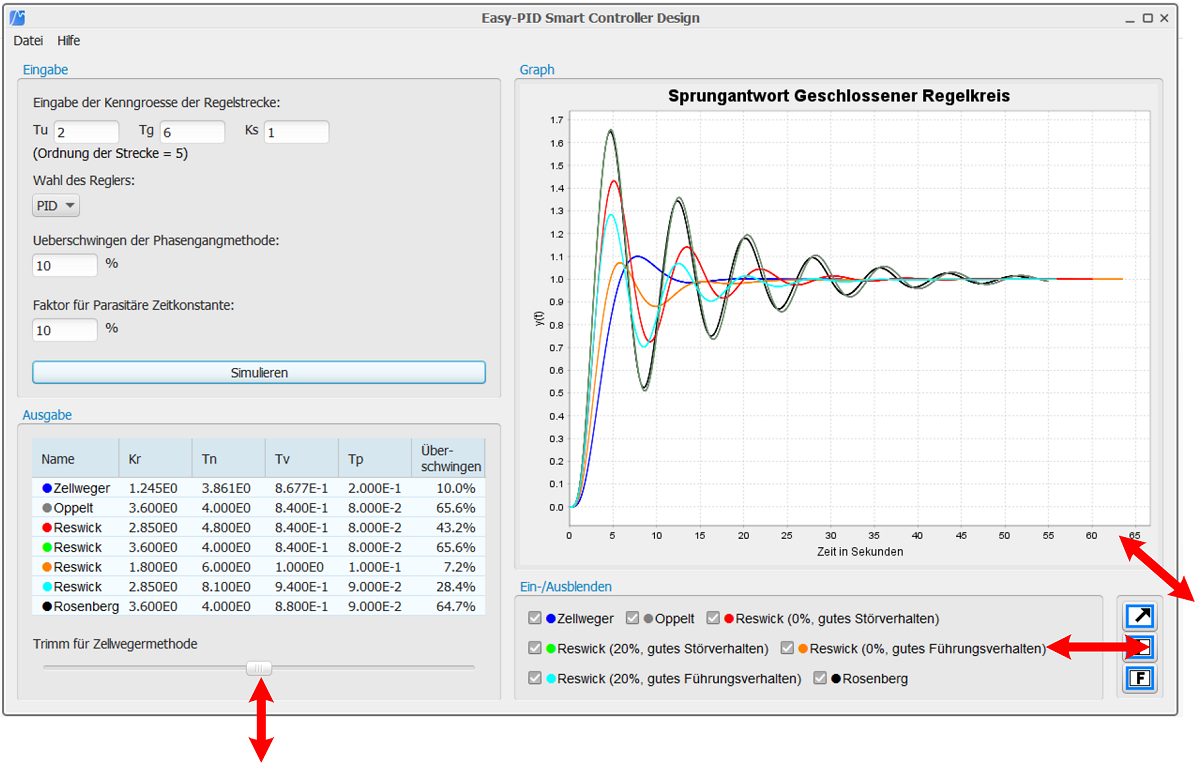
\includegraphics[width=12cm]{ResizeFrame.png}
	\caption{Ver�ndern der Fenstergr�sse}
	\label{fig:Ver�ndern der Fenstergr�sse}
\end{figure}

\textbf{Mini-Version}\\
Durch eine Schaltfl�che in der \textit{MenuBar} kann zur Mini-Version gewechselt werden. Diese reduzierte Ansicht verzichtet auf den Graphen und die dazugeh�rigen Panels und wurde speziell f�r fortgeschrittene Anwender implementiert. Die folgende Grafik zeigt die Mini-Version des Tools.

\begin{figure}[h]
	\centering
		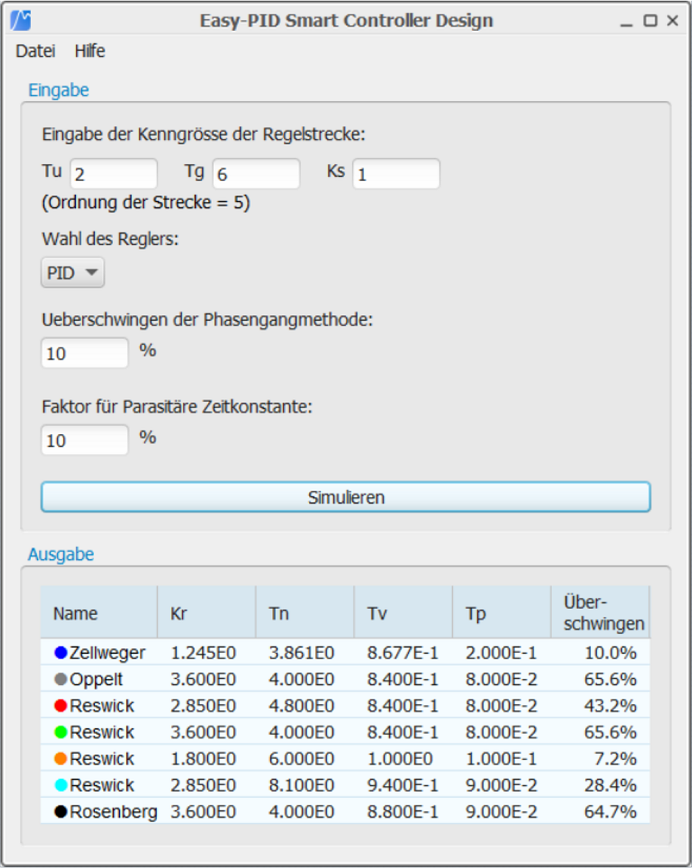
\includegraphics[width=8cm]{Mini-Version.png}
	\caption{Ansicht der Mini-Version}
	\label{fig:Ansicht der Mini-Version}
\end{figure}

%TODO JOSUA:
%- Lesen und ev. korrigieren.
%- Erg�nzen: Textfeldeingaben und Ver�nderung Fenstergr�sse
\subsection{Controller}
%Problem/Fragestellung:
%- Welche Methoden muss der Controller enthalten?
%L�sung: Model und View bestimmen, welche Methoden der Controller enthalten muss.
Der $Controller$ ist sehr schlank gehalten und ist ein Teil des Model-View-Controller-Pattern. Der Controller hat dabei mehrere Aufgaben:
\begin{itemize}
	\item Beim Dr�cken der Simulationsschaltfl�che im \em{InputPanel} werden die entsprechenden Methoden des Models aufgerufen, um die neuen Regler mit den neuen Eingabeparametern zu berechnen, die alten Simulationen zu l�schen und neue Simulationen zu starten. 
	\item Wenn der Trimm-Slider im \em{OutputPanel} ver�ndert wird, so wird die entsprechende Methode im Model aufgerufen. 
	\item Wenn der Anwender eine Checkbox im \em{GraphDisplayPanel} anklickt, wird die entsprechende Methode im Model aufgerufen, um eine Kurve ein- oder auszublenden.  
\end{itemize}

\begin{figure}[h]
	\centering
		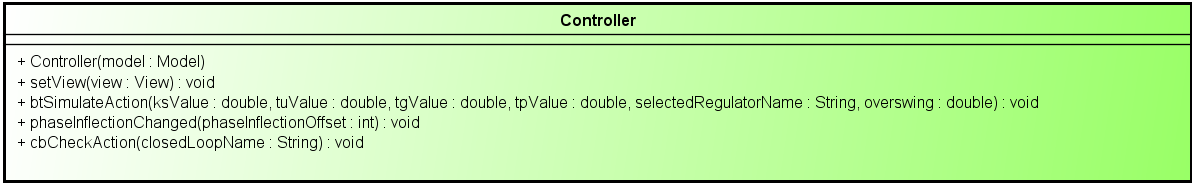
\includegraphics[width=12cm]{Controller_MVC.png}
	\caption{Klasse View}
	\label{fig:Klasse_View}
\end{figure}


%TODO Murray 
%Sehr viele 
%- Korrigieren und ev. erg�nzen.
%- Falls m�glich Text mit weiterem Inhalt erg�nzen. Ev. die Methoden genauer beschreiben und auf die entsprechenden Methoden des Models referenzieren.


\subsection{Ablauf einer Reglerberechnung}
Im folgenden Abschnitt wird die Dimensionierung eines Reglers mit Easy-PID an einem Beispiel erkl�rt. Als Beispiel dient eine Regelstrecke mit den Kenngr�ssen $Tu=2$, $Tg=6$ und $Ks=1$, die parasit�re Zeitkonstante $Tp$ wird bei 10\% belassen, was der Standardeinstellung entspricht. Gew�nscht ist ein PID-Regler mit einem maximalen �berschwingen von 8\%.

\textbf{1.} \\
Die Werte f�r $Tu$, $Tg$ und $Ks$ werden in den entsprechenden \em{JFormattedDoubleTextField} eingegeben, f�r $Tp$ muss nichts eingegeben werden, da 10\% bereits die Standardeinstellung ist. Mit den beiden Dropdown-Men�s, welche mittels \em{JComboBox} implementiert wurden, wird ausserdem der Reglertyp PID und das �berschwingen auf 8\% festgelegt.

\textbf{2.} \\
Durch Dr�cken der Schaltfl�che \em{Simulieren} wird die Methode \em{actionPerformed} aufgerufen, welche die Eingabeparameter in die entsprechenden Attribute speichert. Die Eingabeparameter werden im \em{View} saniert, damit ung�ltige Einstellung m�glichst fr�h erkannt werden k�nnen. Ist alles in Ordnung, wird die Methode \em{Controller::btSimulateAction} aufgerufen. Bei nicht akzeptierten Eingabeparametern erscheint unter den Eingabefeldern ein \em{JLabel} mit der entsprechenden Fehlermeldung. Bei akzeptierten Eingabeparametern wird die Simulation gestartet.

\textbf{3.} \\
Der \em{Controller} konfiguriert das \em{Model}-Objekt mit den Eingabewerten mittels der Methoden \em{Model::set\-Regulator\-Type()} - welche den Typ zu \em{I}, \em{PI} oder \em{PID} setzt, \em{Model::setPlant()} - welche ein neues \em{Plant}-Objekt erstellt und als Attribut der Klasse \em{Model} speichert, \em{Model::set\-Parasitic\-Time\-ConstantFactor()} und \em{Model::setOvershoot()}. Danach ruft sie die Methode \em{Model::simulateAll()} auf, um die Simulation zu beginnen.

\textbf{4.} \\
Das \em{Model} baut sich mit Hilfe seines \em{Plant}-Objekts, welches die vom Benutzer eingegebene Strecke beschreibt, eine Liste von \em{CalculationCycle}-Objekten. Diese Objekte sind dazu f�hig, eine gesamte Berechnung von der Reglerberechnung bis zur Schrittantwort durchzuf�hren. Welche Regler ausgerechnet werden ist abh�ngig von der Auswahl des Reglertyps, also \em{I}, \em{PI} oder \em{PID}.

Es wird mittels \em{Model::notifySimulationBegin()} allen Listener mitgeteilt, dass eine Simulation beginnt. Dies bewirkt unter anderem dass sich die verschiedene Panels auf die Resultate vorbereiten k�nnen, dies umfasst beispielsweise die Tabelle oder den Plot zu l�schen.

Die \em{CalculationCycle}-Klasse erbt von \em{Runnable}. Es wird ein \em{ThreadPool} erstellt und alle \em{CalculationCycle}-Objekte werden parallel ausgef�hrt. Das Programm wartet, bis alle Berechnungen vollendet sind.

\textbf{5.} \\
Zu diesem Zeitpunkt teilt sich der Programmfluss in einer Unmenge kleiner Teilchen auf. Wir verfolgen nur einen Pfad, n�mlich die Berechnung eines PID-Reglers mittels Zellweger Methode.

Beim Instanziieren der Klasse \em{CalculationCycle} wird ein \em{AbstractControllerCalculator} �bergeben. In diesem Fall ist das ein Objekt, dass als konkrete Klasse den \em{ZellwegerPID} hat. Dieses Objekt wurde schon vom \em{Model} konfiguriert und es muss nur \em{AbstractControllerCalculator::run()} aufgerufen werden, um einen passenden Regler f�r die vom Benutzer definierte Strecke zu berechnen. 

\textbf{6.} \\
Die \em{run()}-Methode f�hrt dazu, dass die Methode \em{ZellwegerPID::calculate()} ausgef�hrt wird. Der implementierte Algorithmus von Herrn Zellweger wird in dieser Methode gebraucht, um ein neues \em{ControllerPID}-Objekt zu erstellen. Dieses Objekt beschreibt den Regler Anhand der Reglerparametern $T_n$, $T_v$, $K_r$ und $T_p$ sowie einer �bertragungsfunktion mit der Klasse \em{TransferFunction}. Weiter berechnet das \em{ZellwegerPID}-Objekt einen Minimal- und Maximalwert f�r $K_r$ aus, was sp�ter f�r das Approximieren des �berschwingens gebraucht wird.

\textbf{7.} \\
Der Regler ist berechnet und kann in der \em{CalculationCycle} mit \em{AbstractControllerCalculator::getRegulator()} als \em{AbstractController} geholt werden. Der Regler wird zusammen mit dem \em{Plant}-Objekt zu einem \em{ClosedLoop}-Objekt zusammengef�gt. Das \em{ClosedLoop}-Objekt berechnet aus der Strecke und dem Regler seine eigene \em{TransferFunction} (�bertragungsfunktion).

\textbf{8.} \\
In der \em{CalculationCycle} wird nun die Schrittantwort mit der Methode \em{ClosedLoop::calculate\-Step\-Response()} ausgerechnet. Diese Methode Berechnet mittels Partialbruchzerlegung die Schrittantwort und misst auch gleich das maximale �berschwingen. Wenn der \em{AbstractController} ein Minimal- und Maximalwert f�r $K_r$ ausgerechnet hat, was bei allen Zellweger der Fall ist, dann wird die Schrittantwort mehrmals ausgerechnet, bis das �berschwingen, welches mit der Methode \em{ClosedLoop::getOvershoot()} geholt werden kann, mit dem vom Benutzer definierten Wert �bereinstimmt.

\textbf{9.} \\
Ist die \em{CalculationCycle} abgeschlossen, wird mittels der Methode \em{CalculationCycle::notify\-Step\-Response\-Calculation\-Complete()} allen Listener mitgeteilt, dass die Berechnung einer Schrittantwort fertig ist. Dabei werden die Reglerparameter $K_r$, $T_n$, $T_v$, $T_p$ und das �berschwingen in einer Tabelle im \em{OutputPanel} eingetragen und die Schrittantwort wird in einem 2D-Plot auf der rechten Seite des GUIs in der Klasse \em{GraphPanel} gezeichnet.

\textbf{10.} \\
Wenn der Threadpool keine Jobs mehr hat, dann wird allen Listener mittels der Methode \em{Model::notifySimulationComplete()} mitgeteilt, dass alle Berechnungen beendet sind.

\textbf{11.} \\
Im \em{GraphDisplayPanel} kann mittels der Checkboxen ausgew�hlt werden, welche Schrittantworten visualisiert werden k�nnen, um so einen m�glichst passenden provisorischen Regler zu finden. Das Anklicken der Checkboxen l�st den \em{ActionListener} aus, die in der Klasse \em{GraphDisplayPanel} die Methode \em{actionPerformed} aufruft. Jenachdem ob das \em{JCheckBox} aktiviert ist oder nicht, wird die vom \em{Controller} geh�render Methode \em{cbCheckAction} oder \em{cbUncheckAction} aufgerufen.

Der \em{Controller} selektiert anhand der Methode \em{Model::selectCalculation()} die entsprechende Berechnung aus und ruft dann entweder \em{Model::showSelectedCalculation()} oder \em{Model::hideSelectedCalculation} auf.

Die Klasse \em{Model} merkt sich mit einem Array von boolean-Werte welche Kurven sichtbar sind und welche Kurven unsichtbar sind, damit Kurven zwischen Simulationen ihre Sichtbarkeit behalten. Die Methoden \em{Model::showSelectedCalculation()} und \em{Model::hideSelectedCalculation()} �ndern die entsprechende Werte im Array, und rufen dann \em{Model::notifyShowCalculation()} oder \em{Model::notifyHideCalculation()} auf. Diese Methoden teilen alle Listener mit, dass eine Berechnung sichtbar beziehungsweise unsichtbar gemacht werden sollte.

Dies bewirkt, dass im \em{GraphPanel} die Entsprechende Kurve im Plot unsichtbar beziehungsweise sichtbar gemacht wird.

\textbf{12.} \\
Mittels der \em{JSlider} k�nnen nun die Reglerparameter angepasst werden, wobei sich der Graph im \em{GraphPanel} in Echtzeit den Einstellungen anpasst.

Der \em{JSlider} l�st den Listener-Callback \em{stateChanged} in der Klasse \em{OutputPanel} aus. Dieser ruft die vom \em{Controller} geh�rende Methode \em{angleOfInflectionOffsetChanged()} auf, welche wiederum die Methode \em{Model::updateZellweger()} aufruft.

Das Model speichert f�r jede Simulation den Zellweger-\em{CalculationCycle}-Objekt im Attribut \em{currentZellwegerCalculationCycle} vom \em{Model} damit es sp�ter leicht wieder neu berechnet werden kann.

Mit diesem Objekt wird der neue Winkel im Phasengang dem \em{AbstractZellweger}-Objekt mitgeteilt und die Schrittantwort wird ganz normal wie schon erkl�rt nochmal berechnet.


\section{Validierung}
Im folgenden Abschnitt wird die Validierung beschrieben. Die Validierung dient zum Auffinden und Beheben von Fehlern, um so eine korrekte Funktion des Programms garantieren zu k�nnen. Zum einen wurden die Berechnungen und Simulationen von Matlab �berpr�ft, zum anderen die Software, aufgeteilt in die Teilbereiche Benutzeroberfl�che und Berechnungen.

\subsection{Matlab}

\subsubsection{Programmierung}
%Problem/Fragestellung:
%- Wie kann die korrekte Funktion der Matlab-Programme �berpr�ft werden?
%L�sung: Die berechneten Antworten werden mit den Antworten von Herrn Niklaus verglichen.
Die Berechnung der Regler wurde zuerst mittels m-Files in Matlab implementiert. Zur �berpr�fung der von Matlab gelieferten Werte wurden diese mit den Werten vom Fachcoach Herr Prof. Peter Niklaus verglichen.

\subsubsection{Simulation}
%Problem/Fragestellung:
%- Wie kann die Matlab-Simulation �berpr�ft werden?
%L�sung: Sie wird mit Simulink �berpr�ft.
Mittels Simulink und Matlab wurde der geschlossene Regelkreis simuliert.

\subsection{Java Software}

\subsubsection{Benutzeroberfl�che}
Das Java-Tool wurde jeweils nach einer Implementation eines Elementes und durch die Teammitglieder getestet. Neben gew�hnlichen Eingaben wurde versucht, die Eingabefelder mittels Sonderzeichen und speziellen Werten zu �berlisten. Die Resultierenden Erkenntnisse flossen anschliessend in die Endversion des Java-Tools mit ein. 


%Problem/Fragestellung:
%- Wie k�nnen Probleme oder Konflikte bei der Benutzeroberfl�che ausgeschlossen werden?
%Mehrere unabh�ngige User testen die Software.

%Um die einfache Handhabung der Software zu �berpr�fen wurde die Software im ganzen Projektteam sowie von mehreren unabh�ngigen Benutzern getestet. Die so gefundenen Unklarheiten oder Probleme wurden behoben.

\subsubsection{Model}
%Problem/Fragestellung:
%- Wie wird die korrekte Funktion der Software �berpr�ft?
%L�sung: Die Software mit mit JUnit getestet, wobei die Resultate von Matlab erwartet werden.
Die Plausibilit�t der Schrittantworten konnte relativ einfach optisch mit den Graphen �berpr�ft werden, da das Verhalten der einzelnen Regler bekannt ist. Zur genauen �berpr�fung der einzelnen Klassen wurden s�mtliche Klassen des Models mittels JUnit mit den Ergebnissen von Matlab verglichen.

\subsubsection{Performancevergleich von Partialbruchzerlegung und IFFT}\label{residuenvsifft}
Es wurde festgestellt, dass das Berechnen der Schrittantwort mittels IFFT-Methode langsam ist, vor allem dann, als das iterative Approximieren des �berschwingens implementiert wurde, was dazu f�hrte, dass die Schrittantwortberechnung mehrmals ausgef�hrt werden musste.

Durch Reduzieren der Anzahl Punkte kann die Berechnung beschleunigt werden, jedoch geht dies auf Kosten von Genauigkeit, was anhand des immer zunehmenden Unterschwingens in der Figur \ref{fig:ifft_genauigkeit} zu sehen ist. Weiter sind die Anzahl Punkte bei der IFFT-Methode auf Zahlen der Basis 2 limitiert, was eine genaue Optimierung der Anzahl Punkte unm�glich macht. Durch Experimentieren stellten wir fest, dass ein Minimum von 4096 Punkte f�r ein visuell genaues Resultat gebraucht wird. Dabei konnten wir auf 2048 Punkte f�r das iterative Approximieren des �berschwingens zur�ckgehen. Die Berechnungszeit war aber immer noch merkbar langsam.

\begin{figure}[h]
\centering
\begin{subfigure}{.4\textwidth}
	\centering
	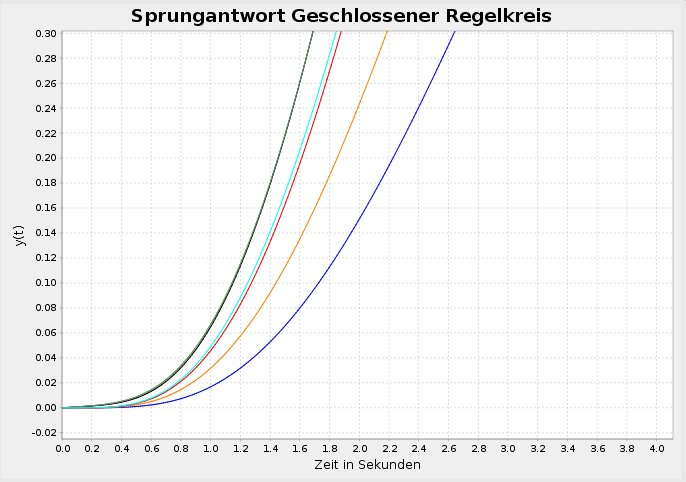
\includegraphics[width=1\linewidth]{./ifft_4096.jpg}
	\caption{Schrittantwort mit 4096 Samples}
	\label{fig:ifft_genauigkeit_4096}
\end{subfigure}
\begin{subfigure}{.4\textwidth}
	\centering
	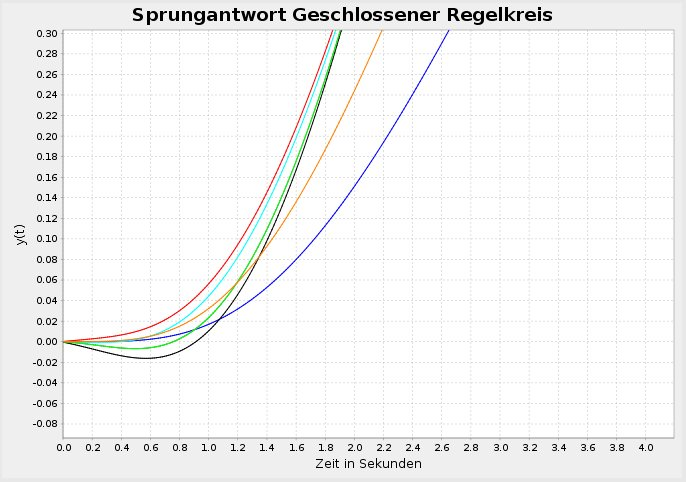
\includegraphics[width=1\linewidth]{./ifft_2048.jpg}
	\caption{Schrittantwort mit 2048 Samples}
	\label{fig:ifft_genauigkeit_2048}
\end{subfigure}
\begin{subfigure}{.4\textwidth}
	\centering
	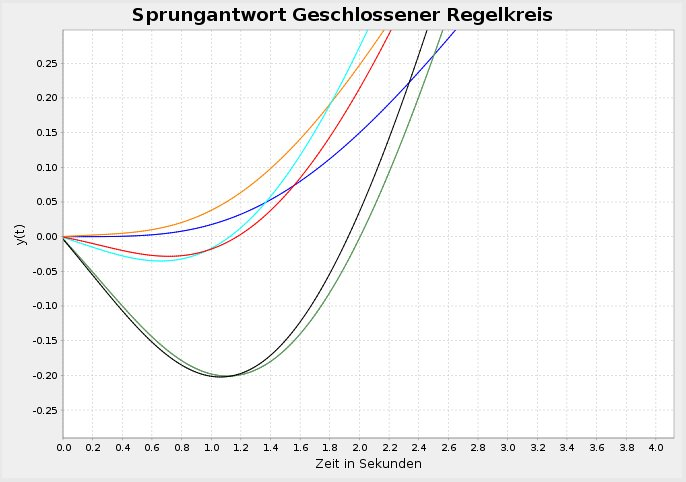
\includegraphics[width=1\linewidth]{./ifft_1024.jpg}
	\caption{Schrittantwort mit 1024 Samples}
    \label{fig:ifft_genauigkeit_1024}
\end{subfigure}
\caption{Vergleich einer IFFT Schrittantwort mit verschiedener Anzahl Punkte}
\label{fig:ifft_genauigkeit}
\end{figure}

Es wurde entschieden, eine alternative Berechnungsmethode zu implementieren: Die Schrittantwortberechnung mittels Partialbruchzerlegung.

Um die Berechnungsgeschwindigkeit beider Methoden messen und vergleichen zu k�nnen, wurden mehrere Tests durchgef�hrt, welche hier im Detail dargelegt werden.

Die Berechnungszeit wurde mit der Methode \textit{System::currentTimeMillis()} gemessen. Weil die Messresultate stark variieren, wurde die Messung mehrmals mittels einer For-Schleife ausgef�hrt, wie im Java-Code in der Figur \ref{fig:code_for_timing_simulations} zu sehen ist.

\begin{figure}[h]
	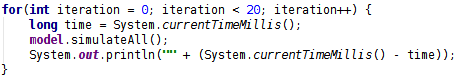
\includegraphics[scale=1]{./code_for_timing_simulations.png}
	\caption{Zeitmessung der Methode \textit{Model::simulateAll()}}
	\label{fig:code_for_timing_simulations}
\end{figure}

Wichtig zu bemerken ist, dass das Programm f�r jede Messung neu gestartet wurde, damit die \textit{Java Virtual Machine} (JVM) ``frisch'' bleibt.

Aus Gr�nden der Reproduzierbarkeit und/oder Vergleichsm�glichkeit wurden die Messungen auf einem System mit folgenden Eigenschaften ausgef�hrt.
\begin{itemize}
	\item \textbf{OS:} Linux twilight 3.18.12-gentoo
	\item \textbf{Arch:} x86\textunderscore 64
	\item \textbf{CPU:} AMD Phenom(tm) II X6 1090T Processor
	\item \textbf{Java:} Oracle JDK 1.8.0.45, Java HotSpot(TM) 64-Bit Server VM
\end{itemize}

Als erstes wurden beide Methoden mit fix 2048 Punkten verglichen. Das sind bei der IFFT-Methode das Minimum, das gebraucht wird, um ein relativ genaues �berschwingen der Zellweger Methode approximieren zu k�nnen; deswegen die Entscheidung, mit 2048 Punkten zu testen. Wie in der Figur \ref{fig:ifft_vs_pbz_2048} zu sehen ist, leistet die Methode mit Partialbruchzerlegung das gleiche Resultat innert halber Zeit.

\begin{figure}[h]
	\centering
	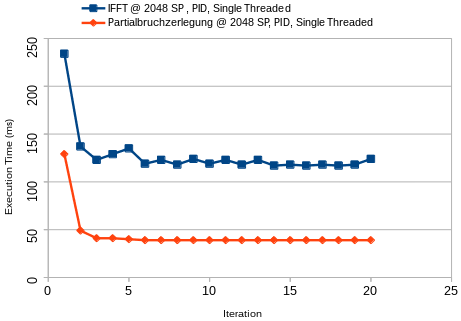
\includegraphics[width=.8\linewidth]{./ifft-vs-partialbruchzerlegung-2048-single-threaded.png}
	\caption{IFFT vs Partialbruchzerlegung mit fix 2048 Samples und keinem Threadpool. Partialbruchzerlegung ist etwa zweimal schneller.}
	\label{fig:ifft_vs_pbz_2048}
\end{figure}

Ein Nachteil der IFFT Methode ist, dass ihre Komplexit�t quadratisch skaliert. Die Partialbruchzerlegungsmethode hingegen skaliert nur linear. Dies ist gut ersichtlich, wenn man Figur \ref{fig:ifft_vs_pbz_2048} und \ref{fig:ifft_vs_pbz_8192} vergleicht.

\begin{figure}[h]
	\centering
	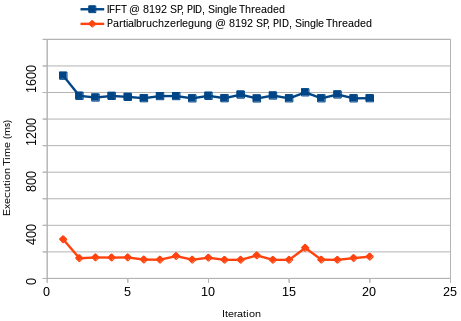
\includegraphics[width=.8\linewidth]{./ifft-vs-partialbruchzerlegung-8192-single-threaded.png}
	\caption{IFFT vs Partialbruchzerlegung mit 8192 Samples und keinem Threadpool. Berechnungszeit von IFFT skaliert quadratisch, Partialbruchzerlegung nur linear.}
	\label{fig:ifft_vs_pbz_8192}
\end{figure}

In der Realit�t braucht die Partialbruchzerlegungsmethode aber viel weniger als 2048 Punkte. Je nachdem was f�r eine Strecke vorliegt, �ndern sich die Anzahl Punkte. Mit einer Strecke von $T_u=2$ und $T_g=6$ wurden in der Figur \ref{fig:pbz-single-vs-multi} nur 145 Punkte gebraucht, was zu einer Berechnungszeit von etwa 8ms f�hrte. Die Berechnung kann mittels Multithreading weiter beschleunigt werden. In diesem Beispiel konnte sie auf weniger als 1ms reduziert werden, wie in Figur \ref{fig:pbz-single-vs-multi} auch zu sehen ist. Man beachte, dass nur 7 Berechnungen parallel liefen. Das heisst, es ist nicht auszuschliessen, dass Multithreading noch schneller sein k�nnte, wenn mehr Berechnungen vorhanden w�ren.

\begin{figure}[h]
	\centering
	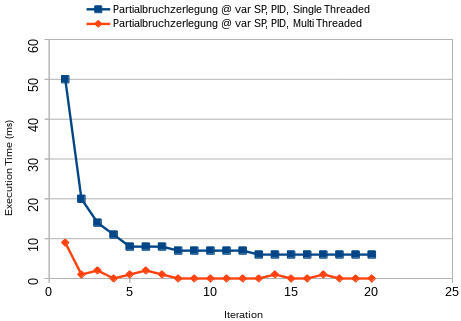
\includegraphics[width=.8\linewidth]{./partialbruchzerlegung-145-single-vs-multi.png}
	\caption{Single Threaded vs Multi Threaded: Partialbruchzerlegung mit variabler Anzahl Samples}
	\label{fig:pbz-single-vs-multi}
\end{figure}


\subsubsection{JUnit-Tests}

\textit{Unit Testing} ist in der Softwareentwicklung ein extrem hilfreiches Verfahren, das den Programmierer erlaubt, individuelle Methoden oder Funktionen isoliert vom Rest des Programms zu testen. Dabei kann f�r jede Methode ein \textit{Test Case} erstellt werden, indem ein Eingabewert und eine Erwartung deklariert werden kann. Das \textit{Unit Testing Framework} - zum Beispiel \textit{JUnit} - f�hrt alle \textit{Test Cases} aus und �berpr�ft dass die Erwarteten Ausgaben den wirklichen Ausgaben entsprechen. Ist dies nicht der Fall, wird ein Fehler generiert.

Der Programmierer kann somit sehr einfach und vorallem schnell schwierige Methoden f�r Richtigkeit �berpr�fen. Der Vorteil von \textit{Unit Testing} liegt darin, dass Methoden nicht nur auf ``richtige'' Eingaben gepr�ft werden k�nnen, sondern auch auf unm�gliche, vielleicht sogar malizi�se Eingaben getested werden k�nnen. Sind die Tests robust, so kann davon ausgegangen werden, dass der Rest des Programms auch robust sein wird.

In den folgenden Bereichen wurde \textit{Unit Testing} anhand des Frameworks \textit{JUnit4} verwendet.

\begin{itemize}
	\item \textbf{ClosedLoop:} Die Schrittantwort wurde direkt mit dem Resultat von Matlab verglichen. Dabei wurde die Kurve von Matlab exportiert und als Liste von XY-Punkte in Java importiert, und mit dem Resultat von \textit{ClosedLoop::calculateStepRespose()} verglichen.
	\item \textbf{In der Klasse \textit{MathStuff}:} Alle Mathematikfunktionen, die von Matlab portiert wurden, sowie zus�tzliche Mathematikfunktionen, die im Laufe des Projekts hinzugef�gt wurden.
	\item \textbf{Faustformeln:} Die von Hand ausgerechnete Resultate wurden mit allen Faustformel-Klassen verglichen.
	\item \textbf{Regler:} Alle Reglerklassen - \textit{ControllerI}, \textit{ControllerPI} und \textit{ControllerPID} - sind mit Matlab verglichen.
	\item \textbf{Strecke:} Die Strecke und deren �bertragungsfunktion wurde mit Matlab verglichen.
	\item \textbf{Sani:} Die Sani-Kurven wurden mit Matlab verglichen.
\end{itemize}


\section{Schlussfolgerung}
%Im Schlusswort wird der Ausgang des Projektes noch einmal revidiert und zusammengefasst. Dabei
%werden die H�he- und Tiefpunkte des Projektes noch einmal erw�hnt.
Easy-PID konnte durchaus erfolgreich abgeschlossen werden. Das Tool erf�llt dabei s�mtliche Anforderungen, welche an ein solches Tool gestellt werden. Einige weitere Funktionen, namentlich die Mini-Version, die Simulation der geschlossenen Regelstrecke und der Export der Berechnung als PDF wurden als Zusatzfunktionen im Programm implementiert. Eine Nachjustierm�glichkeit f�r die Reglerparameter wurde dabei bewusst nicht umgesetzt, jedoch kann mittels eines Schiebereglers die Phasengangmethode optimiert werden.

Der Benutzer kann die Parameter der Regelstrecke in der grafischen Benutzeroberfl�che eingeben, woraufhin Easy-PID die Reglerparameter mittels verschiedener Methoden berechnet und die entsprechenden Sprungantworten grafisch darstellt. Die einzelnen Methoden k�nnen dabei auch ausgeblendet werden. F�r die Phasengangmethode existiert ausserdem ein Trimm-Regler, mit welchem die Phasengangmethode angepasst werden kann. Mit diesen Funktionen erm�glicht es Easy-PID dem Benutzer, den idealen Regler zu dimensionieren.

Das Projekt ist nicht ohne Probleme verlaufen: Das zu Beginn des Projektes aufgestellte Klassendiagramm konnte beispielsweise nicht implementiert werden, da gewisse Aufgaben noch nicht erkannt wurden. Deswegen musste im sp�teren Projektverlauf ein neues Klassendiagramm erstellt werden, welches s�mtliche Aufgaben und Funktionen beachtet und somit gut umgesetzt werden konnte. \\
Ein weiteres Problem war die Umsetzung von Matlab-Code in Java. Viele Funktionen, die in Matlab bereits vorimplementiert sind, mussten f�r das Tool neu programmiert werden. Auch haben die vielen kleinen Unterschiede zwischen den beiden Programmiersprachen immer wieder zu Problemen gef�hrt.

Am Ende konnte das Projekt jedoch termingerecht und korrekt funktionierend abgeliefert werden. Trotzdem gibt es viele Features, welche in zuk�nftigen Projekten noch realisiert werden k�nnten. Eine M�glichkeit w�re das Importieren und Exportieren von Projekten. Dank dem Model-View-Controller Entwurfsmuster kann Easy-PID auch problemlos f�r eine Mobile-App adaptiert werden.

% - Speichern und �ffnen von Projekten
% - Mobile-App
% - 

\begin{appendix}
%\documentclass{fhnwreport} %
%\usepackage[ngerman]{babel}
%\usepackage[T1]{fontenc}
%\usepackage[latin1]{inputenc}
%\usepackage{tikz}
%\usepackage{amsmath}
%\usetikzlibrary{arrows}
%\usepackage{lmodern}   %Type1-Schriftart f�r nicht-englische Texte 
%
%\begin{document}
\section{Anhang Elektrotechnik}

\subsection{Herleitung der Berechnung von $\beta$ f�r die Zellweger Methode}\label{ZellwegerBeta}
F�r den offenen Regelkreis $Go$ gilt:

\begin{center}
	$\phi_{RE}$ Phase Regler

	$\phi_S$ Phase Strecke

	$\phi_O$ Phase offener Regelkreis
	\[
	\phi_{RE}(w_{PID})+\phi_S(w_{PID})=\phi_O(w_{PID})
	\]
\end{center}
F�r die Steigung (Ableitung) gilt:
\begin{equation}
\frac{d\phi_{RE}(w_{PID})}{dw}+\frac{d\phi_S(w_{PID})}{dw}=\frac{d\phi_O(w_{PID})}{dw}
\label{eq:zellwegerPhaseOffenerRegelkreis}
\end{equation}
Der offene Regelkreis berechnet sich wie folgt:
\[
Go=\frac{1}{s\cdot T0\cdot (1+s\cdot T1)}
\]
Die Phase von $O$ berechnet sich wie folgt:
\[
Tk=\frac{1}{w_{PID}}
\]
\[
\phi_O(w_{PID})=-\frac{\pi}{2}-\arctan \left(w\cdot \frac{1}{w_{PID}} \right)=
-\frac{pi}{2}-\arctan \left(w\cdot Tk \right)
\]
$\phi_O$ wird nach $w$ abgeleitet und f�r $Tk$ wird 
$\frac{1}{w_{PID}}$ eingesetzt. Da in $w_{PID}$ abgeleitet 
wurde wird $w$ gleich $w_{PID}$ gesetzt:
\begin{equation}
\frac{d\phi_O(w_{PID})}{dw}=-\frac{Tk}{1+w^{2}\cdot {Tk}^{2}}=-\frac{Tk}{1+{w_{PID}}^{2}\cdot \left( \frac{1}{w_{PID}} 
\right)^{2}}=-\frac{1}{2}Tk=-\frac{1}{2\cdot w_{PID}}
\label{eq:zellwegerPhaseAbleitung}
\end{equation}
Aus der Ableitung der Phase des offenen Regelkreises \eqref{eq:zellwegerPhaseAbleitung} und der Phasengleichung \eqref{eq:zellwegerPhaseOffenerRegelkreis} des offenen Regelkreises folgt:
\[
\phi_{RE}(w_{PID})+\phi_S(w_{PID})=-\frac{1}{2\cdot w_{PID}}
\]
Mit $w_{PID}$ multipliziert
\[
w_{PID} \cdot \frac{d\phi_{RE}(w_{PID})}{dw}+w_{PID} \cdot \frac{d\phi_S(w_{PID})}{dw}=-0.5
\]
Wie man einfach erkennt folgt daraus:
\[
w_{PID} \cdot \frac{d\phi_{RE}(w_{PID})}{dw}=\frac{2\cdot \beta}{1+\beta^{2}}
\]
Eingesetzt in die Phasengleichung:
\[
\frac{2\cdot \beta}{1+\beta^{2}}+w_{PID} \cdot \frac{d\phi_S(w_{PID})}{dw}=-0.5
\]
F�r $\phi_S(w_{PID})$ wird eingesetzt:
\[
\frac{2\cdot \beta}{1+\beta^{2}}+w_{PID} \cdot (-\arctan \left( w_{PID}\cdot T1 
\right)-\arctan \left( w_{PID}\cdot T2 \right)-\arctan \left( w_{PID}\cdot Tz \right))=-0.5
\]

Als Summe geschrieben:
\[
\frac{2\cdot \beta}{1+\beta^{2}}-w_{PID} \cdot  \sum \limits_{m=1}^{N} \arctan \left( w_{PID}\cdot T_m\right) =-0.5
\]

$\phi_S(w_{PID})$ abgeleitet:

\[
\frac{2\cdot \beta}{1+\beta^{2}}-w_{PID} \cdot \left(\frac{T_{1}}{1+ (w_{PID} \cdot T_{2})^2}+\frac{T_{2}}{1+ (w_{PID} \cdot T_{2})^2}+\frac{T_{m}}{1+ (w_{PID} \cdot T_{m})^2}\right)=-0.5
\]

Als Summe geschrieben:

\[
\frac{2\cdot \beta}{1+\beta^{2}}-w_{PID} \cdot  \sum \limits_{m=1}^{N} \frac{T_m}{1+ (w_{PID} \cdot T_m)^2} =-0.5
\]

Nun wird so umgeformt, dass alle $\beta$ auf einer Seite stehen:

\[
\frac{2\cdot \beta}{1+\beta^{2}}=w_{PID} \cdot  \sum \limits_{m=1}^{N} \frac{T_m}{1+ (w_{PID} \cdot T_m)^2} -0.5
\]

Die rechte Seite wird mit $Z$ substituiert:

\[
Z=w_{PID} \cdot  \sum \limits_{m=1}^{N} \frac{T_m}{1+ (w_{PID} \cdot T_m)^2} -0.5
\]

\[
Z=\frac{2\cdot \beta}{1+\beta^{2}}
\]

Nach $\beta$ aufgel�st:
\[
\beta = \frac{1}{Z} - \sqrt{\frac{1}{Z^2}-1}
\]

%\end{document}

%\documentclass{fhnwreport} %
%\usepackage[ngerman]{babel}
%\usepackage[T1]{fontenc}
%\usepackage[latin1]{inputenc}
%\usepackage{tikz}
%\usepackage{amsmath}
%\usetikzlibrary{arrows}
%\usepackage{lmodern}   %Type1-Schriftart f�r nicht-englische Texte 
%
%\begin{document}


\subsection[Herleitung Bodekonforme Darstellung]{Herleitung der Bodekonformen und Reglerkonformen Darstellung}\label{Bodekonf}

Regler k�nnen in verschieden Darstellungen abgebildet werden. Unterschieden werden hier die reglerkonforme und die bodekonforme Darstellung, wobei oftmals standartm�ssig die reglerkonforme Darstellung gew�hlt wird. Folgend sind beide Darstellungen von PI- und PID-Regler aufgef�hrt. Beim PID-Regler wird zudem die Beziehung zwischen den beiden Formen hergeleitet.

\subsubsection{PI-Regler}
Der PI-Regler hat die Parameter $Kr$ und $Tn$.
\par \textbf{Reglerkonform:} %use \par for next line, use \\ or \newline for a new line
\begin{equation}
G_{R}(s) = K_{R}\left(1+\frac{1}{s\cdot Tn}\right)
\end{equation}


\textbf{Bodekonform:}
\begin{equation}
G_{R}(s) = K_{R}\left(\frac{1+s\cdot Tn}{s\cdot Tn}\right)
\end{equation}

\subsubsection{PID-Regler}
\textbf{Reglerkonform:}
\par Der PID-Regler hat in der reglerkonformen Darstellung die Parameter $Kr$, $Tn$, $Tv$ und $Tp$.
\begin{equation}
G_{R}(s) = K_{R}\left(1+\frac{1}{s\cdot Tn}+\frac{s\cdot Tv}{1+s\cdot Tp}\right)
\end{equation}
Umformung:

\begin{equation}
\begin{aligned} % use {aligned} and &= to aligne vertical all = 
	G_{R}(s) &= K_{R}\left(\frac{s \cdot Tn(1+s \cdot Tp) + (1+s \cdot Tp)(s \cdot Tn \cdot s \cdot Tv)}{s \cdot Tn(1+s \cdot Tp)}\right) \\ 
	&= K_{R}\left(\frac{s^2 \cdot Tn\cdot Tp + s^2 \cdot Tn \cdot Tv + s \cdot Tp + s \cdot Tn + 1}{s \cdot Tn(1+s \cdot Tp)}\right) \\
	&= K_{R}\left(\frac{s^2(Tn\cdot Tp + Tn \cdot Tv) + s(Tp + Tn) + 1 }{s \cdot Tn(1+s \cdot Tp)}\right) 
	\\
	&= K_{R}\left(\frac{s^2\cdot Tn(Tp + Tv) + s(Tp + Tn) + 1 }{s \cdot Tn(1+s \cdot Tp)}\right)
\end{aligned}
\end{equation}


\textbf{Bodekonform:}
\par Der PID-Regler hat in der bodekonformen Darstellung die Parameter $Krk$, $Tn$, $Tv$ und $Tp$.
\begin{equation}
G_{R}(s) = K_{RK}\left(\frac{(1+s\cdot Tnk)(1+s\cdot Tvk)}{s\cdot Tnk(1+s\cdot Tp)}\right)
\end{equation}
Umformung:

\begin{equation}
\begin{aligned} 
G_{R}(s) = K_{RK}\left(\frac{s^2(Tnk \cdot Tvk)+ s(Tnk + Tnk) + 1}{s\cdot Tnk(1+s\cdot Tp)}\right)
\end{aligned}
\end{equation}

\par \textbf{Koeffizienten-Vergleich:}
\\Damit ein Koeffizienten-Vergleich zwischen der reglerkonformen und der bodekonformen Darstellung des PID-Reglers durchgef�hrt werden kann, m�ssen die beiden Formen gleichgesetzt werden (links reglerkonform, rechts bodekonform):

\begin{align}
K_{R}\left(\frac{s^2\cdot Tn(Tp + Tv) + s(Tp + Tn) + 1 }{s \cdot Tn(1+s \cdot Tp)}\right) &= K_{RK}\left(\frac{s^2(Tnk \cdot Tvk)+ s(Tnk + Tnk) + 1}{s\cdot Tnk(1+s\cdot Tp)}\right) \nonumber \\  %\textcolor[rgb]{1,0,0}{s}
\intertext{$s$  wird auf beiden Seiten im Nenner gek�rzt:} \nonumber
K_{R}\left(\frac{s^2\cdot Tn(Tp + Tv) + s(Tp + Tn) + 1 }{Tn(1+s \cdot Tp)}\right)&= K_{RK}\left(\frac{s^2(Tnk \cdot Tvk)+ s(Tnk + Tnk) + 1}{Tnk(1+s\cdot Tp)}\right) \\
\intertext{L�sst man die Frequenz $w$ gegen Null gehen, strebt auch $s$ gegen Null und die Terme lassen sich wie folgt vereinfachen:} \nonumber 
K_{R}\left(\frac{ 1 }{Tn}\right)&= K_{RK}\left(\frac{1}{Tnk}\right)
\end{align}

An der oben stehenden Umformung erkennt man, dass man einen Koeffizientenvergleich machen kann. Folgend werden zuerst die Koeffizienten mit $s$, danach die $s^2$ und am Ende die Koeffizienten ohne $s$ verglichen und nach den Parameter der reglerkonformen Darstellung umgeformt.

2. Koeffizient
\begin{equation}
\begin{aligned}
s(Tn+Tp) &= s(Tnk+Tvk) \\
Tn+Tp &= Tnk+Tvk \\
Tn &= Tnk+Tvk-Tp\\
\label{eq:2koeffizient}
\end{aligned}
\end{equation}

Damit ist $Tn$ bestimmt.

1. Koeffizient:
\begin{equation}
\begin{aligned}
s^2(Tn\cdot Tp + Tn \cdot Tv)&=s^2(Tnk \cdot Tvk)\\
(Tn\cdot Tp + Tn \cdot Tv)&=(Tnk \cdot Tvk)\\
Tn(Tv + Tp)&=Tnk \cdot Tvk
\end{aligned}
\end{equation}

Obenstehende Gleichung wird nun nach $Tv$ umgeformt:

\begin{equation*} %star after equations means NO automatic numbering
\begin{aligned}
Tv + Tp &= \frac{Tnk \cdot Tvk}{Tn}\\
Tv &= \frac{Tnk \cdot Tvk}{Tn} - Tp
\end{aligned}
\end{equation*}

Die Variable $Tn$ wird in der folgenden Gleichung durch die Beziehung von Formel \ref{eq:2koeffizient} ersetzt:

\begin{equation}
\begin{aligned}
Tv &= \frac{Tnk \cdot Tvk}{Tnk+Tvk-Tp} - Tp
\end{aligned}
\end{equation}

Damit ist $Tv$ bestimmt. $Kr$ wird wie folgt bestimmt:

3. Koeffizient:
\begin{align}
\frac{Kr}{s \cdot Tn (1+s\cdot Tp)} &= \frac{Krk}{s\cdot Tnk(1+s\cdot Tp)}\nonumber \\  %\nonumber means no number on this line
\intertext{$s$ und $(1+s\cdot Tp)$ werden gek�rzt und $Tn$ ersetzt:}
\frac{Kr}{Tnk+Tvk-Tp} &= \frac{Krk}{Tnk}\nonumber \\ 
Kr &= \frac{Krk(Tnk+Tvk-Tp)}{Tnk}\nonumber \\ 
\intertext{Das im Verh�ltnis zu $Tvk$ ca. zehn mal kleinere $Tp$ kann vernachl�ssigt werden:}
Kr &= \frac{Krk(Tnk+Tvk)}{Tnk} \nonumber \\ 
Kr &= \frac{Krk(1+Tvk)}{Tnk}
\end{align}

%\begin{equation}
%Tn = \frac{Tnk \cdot Tvk}{Tvk + Tp}
%\end{equation}



%Jetzt wird $Tn$ in $Tv$ eingesetzt:
%\begin{equation}
%\begin{aligned}
%Tv &= \frac{Tnk \cdot Tvk (Tv + Tp}{Tnk \cdot Tvk} - Tp
%\end{aligned}
%\end{equation}



%\end{document}


\bibliography{Literature}
%\include{./Software/LatexSoftware/Anhang_Software}
%\section{Klassendiagramm}\label{klassendiagramm}
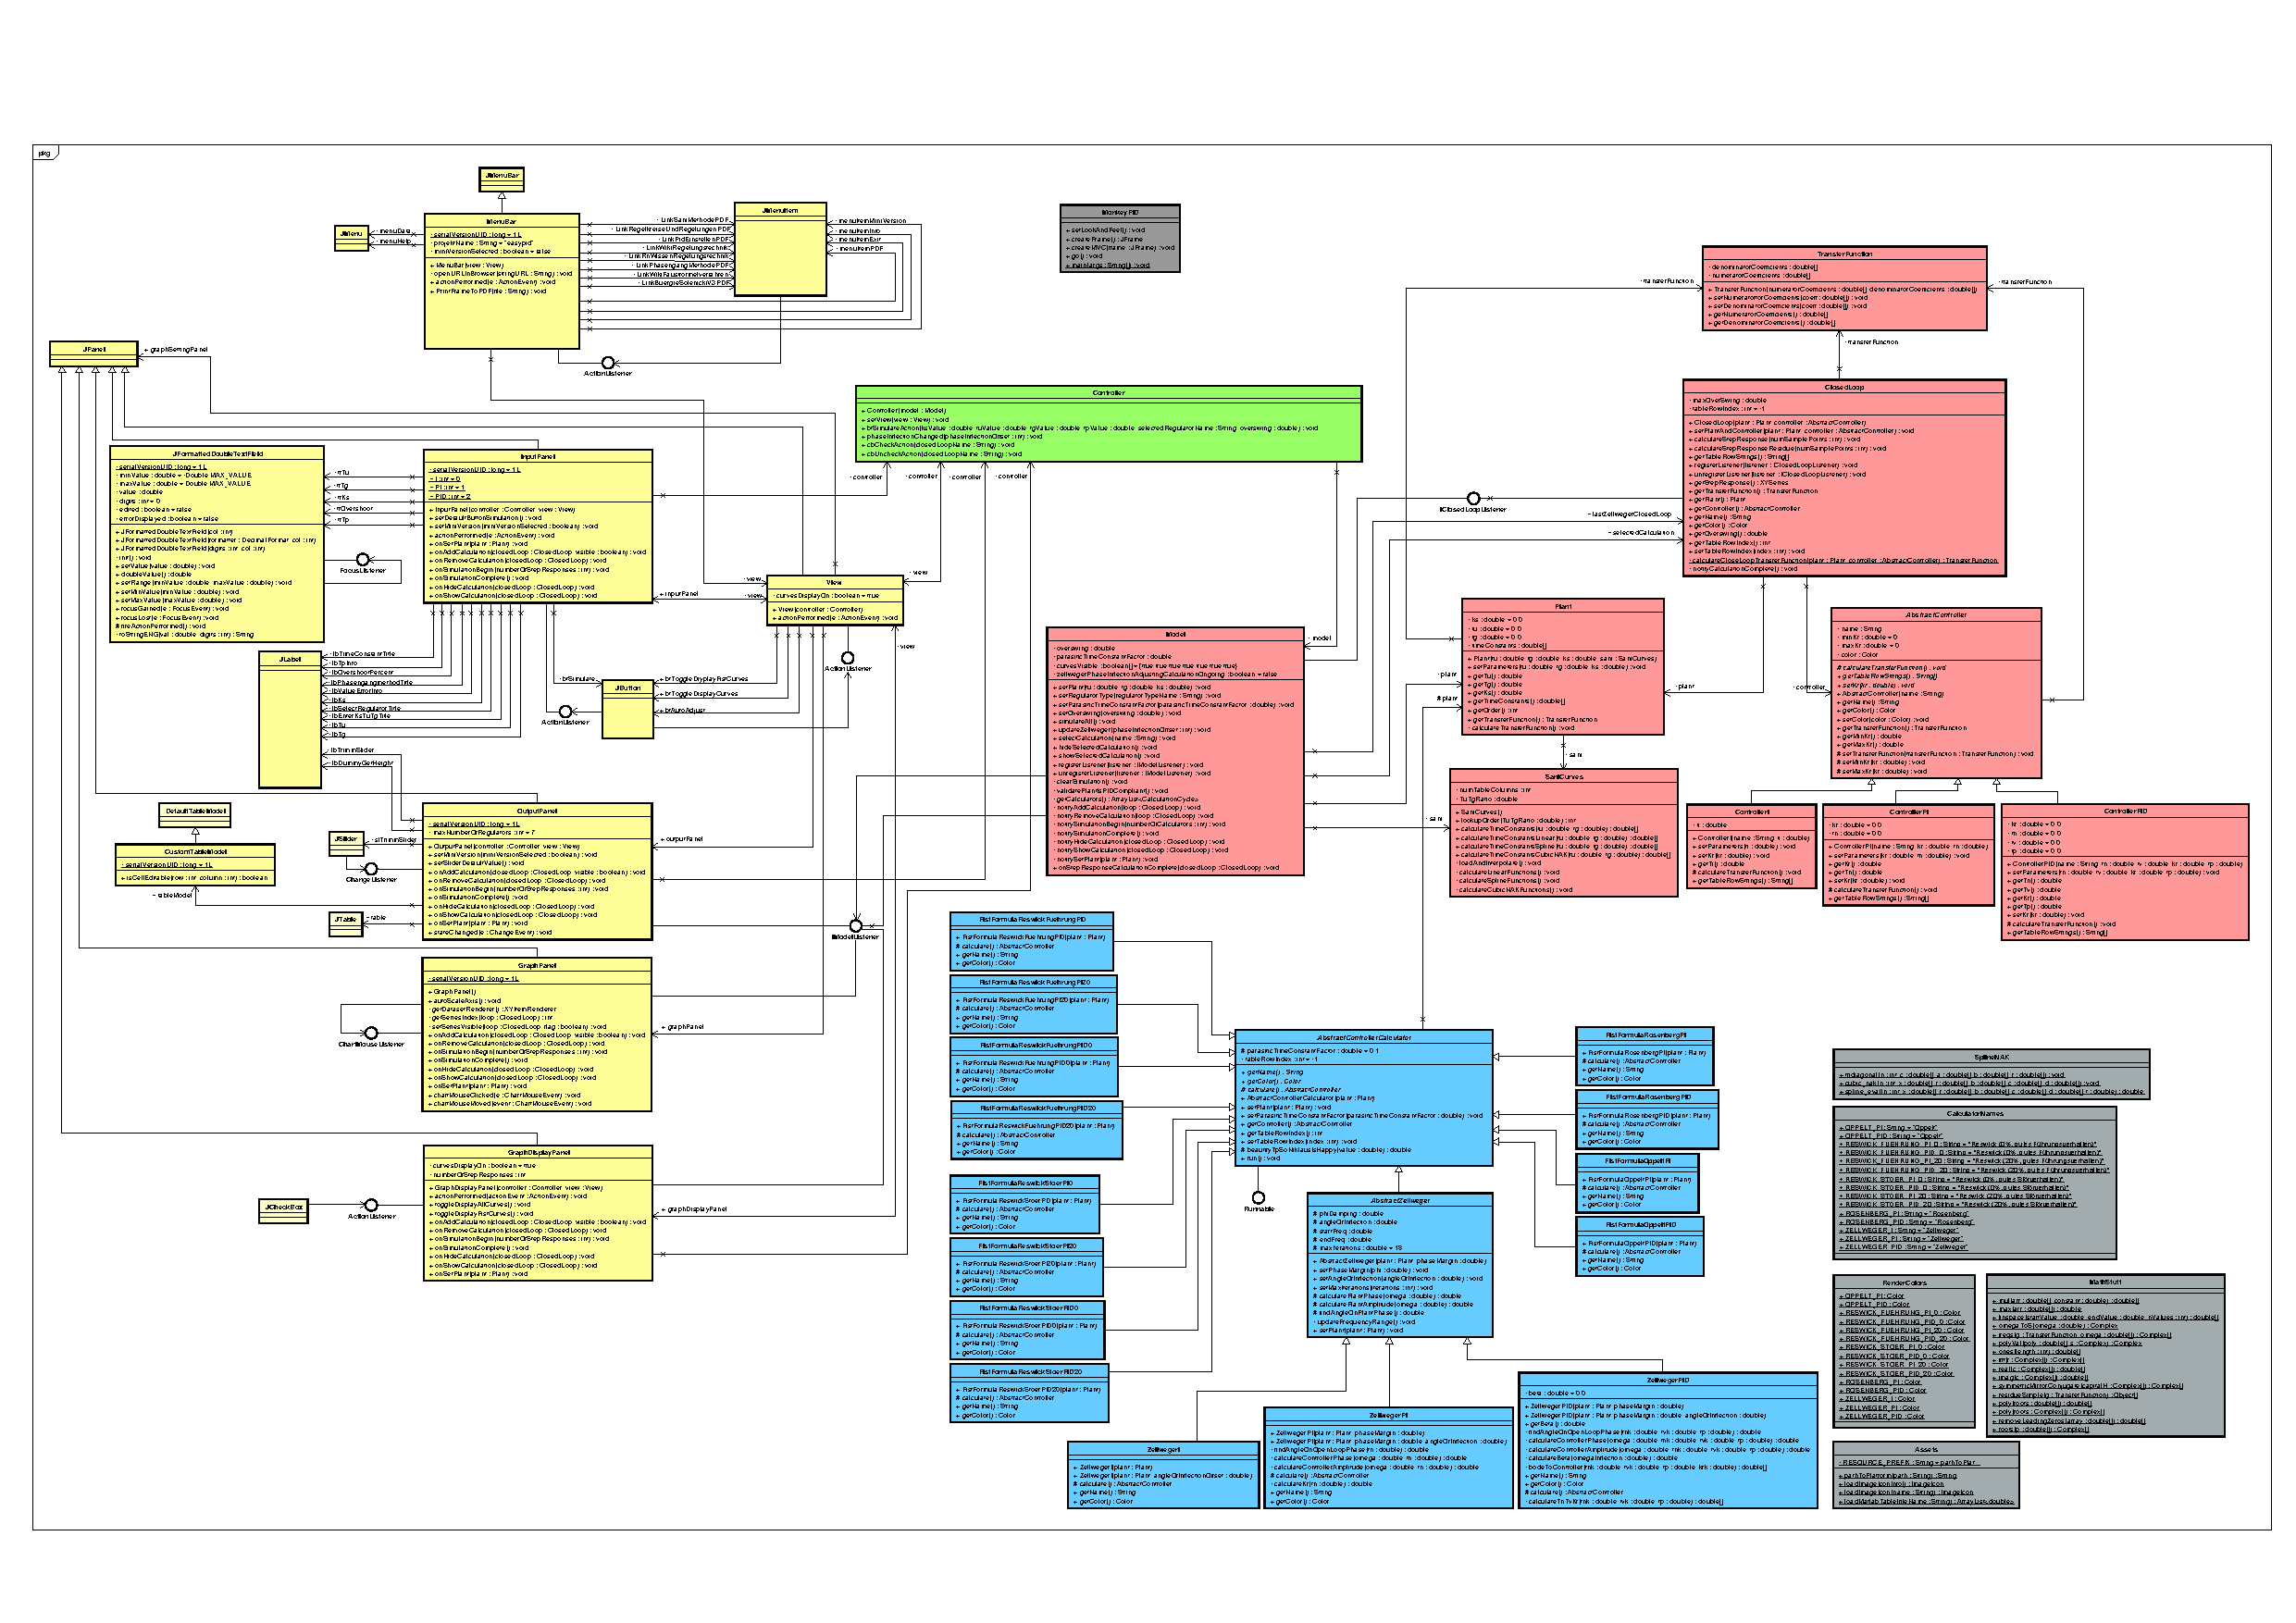
\includepdf[% 
   fitpaper=true, 
]{Class_Diagramm_V03.pdf}
\section{CD-Rom}
\end{appendix}
\end{document}